% Options for packages loaded elsewhere
\PassOptionsToPackage{unicode}{hyperref}
\PassOptionsToPackage{hyphens}{url}
%
\documentclass[
]{book}
\usepackage{amsmath,amssymb}
\usepackage{iftex}
\ifPDFTeX
  \usepackage[T1]{fontenc}
  \usepackage[utf8]{inputenc}
  \usepackage{textcomp} % provide euro and other symbols
\else % if luatex or xetex
  \usepackage{unicode-math} % this also loads fontspec
  \defaultfontfeatures{Scale=MatchLowercase}
  \defaultfontfeatures[\rmfamily]{Ligatures=TeX,Scale=1}
\fi
\usepackage{lmodern}
\ifPDFTeX\else
  % xetex/luatex font selection
\fi
% Use upquote if available, for straight quotes in verbatim environments
\IfFileExists{upquote.sty}{\usepackage{upquote}}{}
\IfFileExists{microtype.sty}{% use microtype if available
  \usepackage[]{microtype}
  \UseMicrotypeSet[protrusion]{basicmath} % disable protrusion for tt fonts
}{}
\makeatletter
\@ifundefined{KOMAClassName}{% if non-KOMA class
  \IfFileExists{parskip.sty}{%
    \usepackage{parskip}
  }{% else
    \setlength{\parindent}{0pt}
    \setlength{\parskip}{6pt plus 2pt minus 1pt}}
}{% if KOMA class
  \KOMAoptions{parskip=half}}
\makeatother
\usepackage{xcolor}
\usepackage{color}
\usepackage{fancyvrb}
\newcommand{\VerbBar}{|}
\newcommand{\VERB}{\Verb[commandchars=\\\{\}]}
\DefineVerbatimEnvironment{Highlighting}{Verbatim}{commandchars=\\\{\}}
% Add ',fontsize=\small' for more characters per line
\usepackage{framed}
\definecolor{shadecolor}{RGB}{248,248,248}
\newenvironment{Shaded}{\begin{snugshade}}{\end{snugshade}}
\newcommand{\AlertTok}[1]{\textcolor[rgb]{0.94,0.16,0.16}{#1}}
\newcommand{\AnnotationTok}[1]{\textcolor[rgb]{0.56,0.35,0.01}{\textbf{\textit{#1}}}}
\newcommand{\AttributeTok}[1]{\textcolor[rgb]{0.13,0.29,0.53}{#1}}
\newcommand{\BaseNTok}[1]{\textcolor[rgb]{0.00,0.00,0.81}{#1}}
\newcommand{\BuiltInTok}[1]{#1}
\newcommand{\CharTok}[1]{\textcolor[rgb]{0.31,0.60,0.02}{#1}}
\newcommand{\CommentTok}[1]{\textcolor[rgb]{0.56,0.35,0.01}{\textit{#1}}}
\newcommand{\CommentVarTok}[1]{\textcolor[rgb]{0.56,0.35,0.01}{\textbf{\textit{#1}}}}
\newcommand{\ConstantTok}[1]{\textcolor[rgb]{0.56,0.35,0.01}{#1}}
\newcommand{\ControlFlowTok}[1]{\textcolor[rgb]{0.13,0.29,0.53}{\textbf{#1}}}
\newcommand{\DataTypeTok}[1]{\textcolor[rgb]{0.13,0.29,0.53}{#1}}
\newcommand{\DecValTok}[1]{\textcolor[rgb]{0.00,0.00,0.81}{#1}}
\newcommand{\DocumentationTok}[1]{\textcolor[rgb]{0.56,0.35,0.01}{\textbf{\textit{#1}}}}
\newcommand{\ErrorTok}[1]{\textcolor[rgb]{0.64,0.00,0.00}{\textbf{#1}}}
\newcommand{\ExtensionTok}[1]{#1}
\newcommand{\FloatTok}[1]{\textcolor[rgb]{0.00,0.00,0.81}{#1}}
\newcommand{\FunctionTok}[1]{\textcolor[rgb]{0.13,0.29,0.53}{\textbf{#1}}}
\newcommand{\ImportTok}[1]{#1}
\newcommand{\InformationTok}[1]{\textcolor[rgb]{0.56,0.35,0.01}{\textbf{\textit{#1}}}}
\newcommand{\KeywordTok}[1]{\textcolor[rgb]{0.13,0.29,0.53}{\textbf{#1}}}
\newcommand{\NormalTok}[1]{#1}
\newcommand{\OperatorTok}[1]{\textcolor[rgb]{0.81,0.36,0.00}{\textbf{#1}}}
\newcommand{\OtherTok}[1]{\textcolor[rgb]{0.56,0.35,0.01}{#1}}
\newcommand{\PreprocessorTok}[1]{\textcolor[rgb]{0.56,0.35,0.01}{\textit{#1}}}
\newcommand{\RegionMarkerTok}[1]{#1}
\newcommand{\SpecialCharTok}[1]{\textcolor[rgb]{0.81,0.36,0.00}{\textbf{#1}}}
\newcommand{\SpecialStringTok}[1]{\textcolor[rgb]{0.31,0.60,0.02}{#1}}
\newcommand{\StringTok}[1]{\textcolor[rgb]{0.31,0.60,0.02}{#1}}
\newcommand{\VariableTok}[1]{\textcolor[rgb]{0.00,0.00,0.00}{#1}}
\newcommand{\VerbatimStringTok}[1]{\textcolor[rgb]{0.31,0.60,0.02}{#1}}
\newcommand{\WarningTok}[1]{\textcolor[rgb]{0.56,0.35,0.01}{\textbf{\textit{#1}}}}
\usepackage{longtable,booktabs,array}
\usepackage{calc} % for calculating minipage widths
% Correct order of tables after \paragraph or \subparagraph
\usepackage{etoolbox}
\makeatletter
\patchcmd\longtable{\par}{\if@noskipsec\mbox{}\fi\par}{}{}
\makeatother
% Allow footnotes in longtable head/foot
\IfFileExists{footnotehyper.sty}{\usepackage{footnotehyper}}{\usepackage{footnote}}
\makesavenoteenv{longtable}
\usepackage{graphicx}
\makeatletter
\def\maxwidth{\ifdim\Gin@nat@width>\linewidth\linewidth\else\Gin@nat@width\fi}
\def\maxheight{\ifdim\Gin@nat@height>\textheight\textheight\else\Gin@nat@height\fi}
\makeatother
% Scale images if necessary, so that they will not overflow the page
% margins by default, and it is still possible to overwrite the defaults
% using explicit options in \includegraphics[width, height, ...]{}
\setkeys{Gin}{width=\maxwidth,height=\maxheight,keepaspectratio}
% Set default figure placement to htbp
\makeatletter
\def\fps@figure{htbp}
\makeatother
\setlength{\emergencystretch}{3em} % prevent overfull lines
\providecommand{\tightlist}{%
  \setlength{\itemsep}{0pt}\setlength{\parskip}{0pt}}
\setcounter{secnumdepth}{5}
\usepackage{booktabs}
\ifLuaTeX
  \usepackage{selnolig}  % disable illegal ligatures
\fi
\usepackage[]{natbib}
\bibliographystyle{plainnat}
\usepackage{bookmark}
\IfFileExists{xurl.sty}{\usepackage{xurl}}{} % add URL line breaks if available
\urlstyle{same}
\hypersetup{
  pdftitle={ADS - Tecnologia da Informação e Telecomunicações 2025 - Anotações de aula},
  pdfauthor={Professor Miguel Suez Xve Penteado},
  hidelinks,
  pdfcreator={LaTeX via pandoc}}

\title{ADS - Tecnologia da Informação e Telecomunicações 2025 - Anotações de aula}
\author{Professor Miguel Suez Xve Penteado}
\date{2025-05-05}

\begin{document}
\maketitle

{
\setcounter{tocdepth}{1}
\tableofcontents
}
\chapter*{Sobre estas anotações}\label{sobre-estas-anotauxe7uxf5es}
\addcontentsline{toc}{chapter}{Sobre estas anotações}

Estas anotações são apenas lembretes das aulas expostas em sala, durante a disciplina de ENGENHARIA DE SOFTWARE.

\subsection{ACESSO Anotações de aula no ceular (github)}\label{acesso-anotauxe7uxf5es-de-aula-no-ceular-github}

\url{https://miguel7penteado.github.io/ADS-TecnologiaInformacaoComunicacoes2025/}

\includegraphics{images/qr-code/repositório.jpg}

\subsection{Anotações de aula: Suporte para Celulares}\label{anotauxe7uxf5es-de-aula-suporte-para-celulares}

No celular o conteúdo pode ser lido no formato EPUB, sendo sugerio os seguintes aplicativos:

\subsection{\texorpdfstring{\textbf{Moon+ Reader (Google Play - loja de aplicativos oficial do google)}}{Moon+ Reader (Google Play - loja de aplicativos oficial do google)}}\label{moon-reader-google-play---loja-de-aplicativos-oficial-do-google}

\url{https://play.google.com/store/apps/details?id=com.flyersoft.moonreader&pcampaignid=web_share}


\includegraphics{images/qr-code/leitor_ebook/MoonReaderPlus.jpg}

\subsection{\texorpdfstring{\textbf{Epub Reader (AppStore - loja de aplicativos oficial da Apple)}}{Epub Reader (AppStore - loja de aplicativos oficial da Apple)}}\label{epub-reader-appstore---loja-de-aplicativos-oficial-da-apple}

\url{https://apps.apple.com/br/app/epub-leitor-ler-epub-chm-txt/id1296870631?platform=iphone}


\includegraphics{images/qr-code/leitor_ebook/AppleEpubReader.jpg}

\chapter*{INTRODUÇÃO DA DISCIPLINA}\label{introduuxe7uxe3o-da-disciplina}
\addcontentsline{toc}{chapter}{INTRODUÇÃO DA DISCIPLINA}

coming soon

\section{Livros-Texto da disciplina}\label{livros-texto-da-disciplina}

\subsection{Bibliografia Básica}\label{bibliografia-buxe1sica}

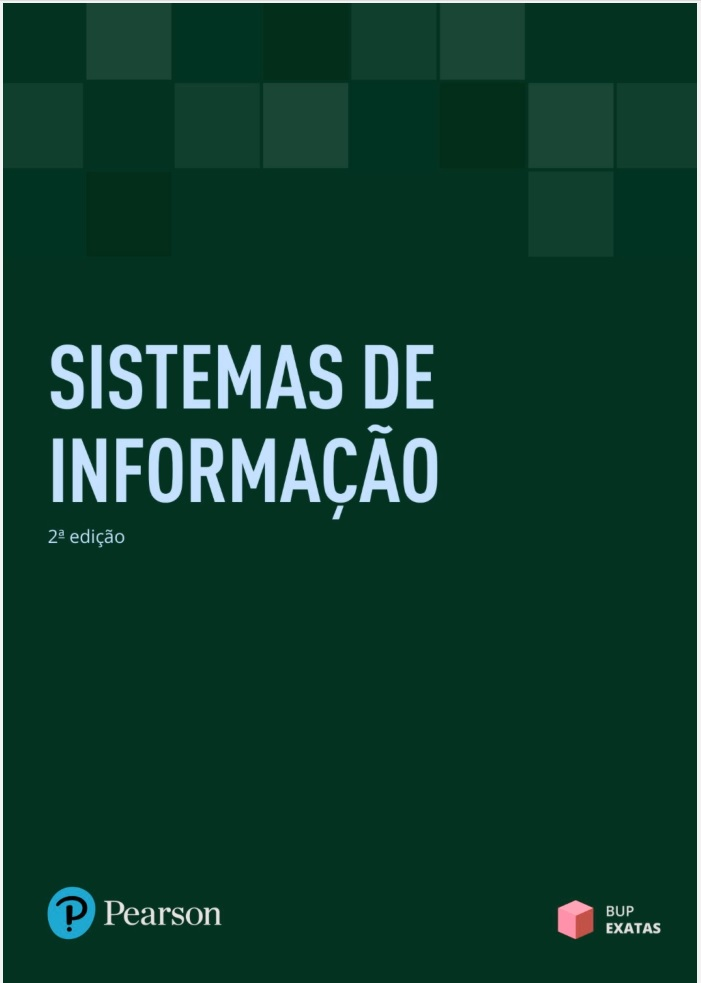
\includegraphics[width=3.03125in,height=\textheight]{images/livros/livro-SistemasDeInformação-BelmiroNascimentoJoao-2ed-person.jpg}

( JOÃO, Belmiro N. Sistemas de Informação - São Paulo: Pearson Education do Brasil, 2019.)

JOÃO, Belmiro N. Informática Aplicada. São Paulo: Pearson Education do Brasil, 2019.

GONÇALVES, G. R. B. Sistemas de informação. Porto Alegre: SAGAH, 2017.

SILVA, K. C. N.; BARBOSA, C.; CÓRDOVA JUNIOR, R. S. Sistemas de informações gerenciais. Porto Alegre: SAGAH, 2018.

\subsection{Bibliografia Complementar}\label{bibliografia-complementar}

LAUDON, Kenneth C; LAUDON, Jane P. Sistemas de Informação Gerenciais. São Paulo: Pearson Education do Brasil, 2014.

MUNHOZ, Antônio S. Fundamentos de Tecnologia da Informação e análise de sistemas para não analistas. Curitiba: Intersaberes, 2017.

MARÇULA, M.; BENINI FILHO, P. A. Informática: Conceitos e Aplicações. 5.Ed. São Paulo: Erica: 2019.

RAINER JUNIOR, R. K.; CEGIELSKI, C. G. Introdução a sistemas de informação. - 5. ed.~- Rio de Janeiro: Elsevier, 2016.

STAIR, Ralph M; REYNOLDS, George W. Princípios de sistemas de informação / Ralph M. Stair. São Paulo: Cengage Learning, 2015.

\section{CALENDÁRIO DE AULAS E PROVAS}\label{calenduxe1rio-de-aulas-e-provas}

\subsection{Chácara Santo Antônio}\label{chuxe1cara-santo-antuxf4nio}

\textbf{Fevereiro 2025}

\begin{longtable}[]{@{}cccc@{}}
\toprule\noalign{}
No. & fevereiro 2025 & Semana & conteúdo \\
\midrule\noalign{}
\endhead
\bottomrule\noalign{}
\endlastfoot
01 & 17/02/2025 & Segunda-feira & Inaugural \\
02 & 24/02/2025 & Segunda-feira & Aula 01 \\
\end{longtable}

\textbf{Março 2025}

\begin{longtable}[]{@{}cccc@{}}
\toprule\noalign{}
No. & Março 2025 & Semana & conteúdo \\
\midrule\noalign{}
\endhead
\bottomrule\noalign{}
\endlastfoot
03 & 03/03/2025 & Segunda-feira & Feriado \\
04 & 10/03/2025 & Segunda-feira & Aula 02 \\
05 & 17/03/2025 & Segunda-feira & Aula 03 \\
06 & 24/03/2025 & Segunda-feira & Aula 04 \\
07 & 31/03/2025 & Segunda-feira & NP1 \\
\end{longtable}

\textbf{Abril 2025}

\begin{longtable}[]{@{}cccc@{}}
\toprule\noalign{}
No. & Abril 2025 & Semana & conteúdo \\
\midrule\noalign{}
\endhead
\bottomrule\noalign{}
\endlastfoot
08 & 07/04/2025 & Segunda-feira & Aula 05 \\
09 & 14/04/2025 & Segunda-feira & Aula 06 \\
10 & 21/04/2025 & Segunda-feira & Aula 07 \\
11 & 28/04/2025 & Segunda-feira & Aula 08 \\
\end{longtable}

\textbf{maio 2025}

\begin{longtable}[]{@{}cccc@{}}
\toprule\noalign{}
No. & Maio 2025 & Semana & conteúdo \\
\midrule\noalign{}
\endhead
\bottomrule\noalign{}
\endlastfoot
12 & 05/05/2025 & Segunda-feira & Aula 09 \\
13 & 12/05/2025 & Segunda-feira & Aula 10 \\
14 & 19/05/2025 & Segunda-feira & NP2 \\
15 & 26/05/2025 & Segunda-feira & SUB \\
\end{longtable}

\textbf{junho 2025}

\begin{longtable}[]{@{}cccc@{}}
\toprule\noalign{}
No. & Junho 2025 & Semana & conteúdo \\
\midrule\noalign{}
\endhead
\bottomrule\noalign{}
\endlastfoot
12 & 02/06/2025 & Segunda-feira & PLANTÃO \\
13 & 09/06/2025 & Segunda-feira & PLANTÃO \\
14 & 16/06/2025 & Segunda-feira & EXAME \\
15 & 23/06/2025 & Segunda-feira & VISTAS \\
\end{longtable}

\subsection{Marquês de São Vicente}\label{marquuxeas-de-suxe3o-vicente}

\textbf{Fevereiro 2025}

\begin{longtable}[]{@{}cccc@{}}
\toprule\noalign{}
No. & Fevereiro 2025 & Semana & conteúdo \\
\midrule\noalign{}
\endhead
\bottomrule\noalign{}
\endlastfoot
1 & 05/02/2025 & Quarta-feira & \\
1 & 05/02/2025 & Quarta-feira & \\
2 & 12/02/2025 & Quarta-feira & \\
3 & 19/02/2025 & Quarta-feira & Inaugural \\
4 & 26/02/2025 & Quarta-feira & Aula 01 \\
\end{longtable}

\textbf{Março 2025}

\begin{longtable}[]{@{}cccc@{}}
\toprule\noalign{}
No. & Março 2025 & Semana & conteúdo \\
\midrule\noalign{}
\endhead
\bottomrule\noalign{}
\endlastfoot
5 & 05/03/2025 & Quarta-feira & Feriado \\
6 & 12/03/2025 & Quarta-feira & Aula 02 \\
7 & 19/03/2025 & Quarta-feira & Aula 03 \\
8 & 26/03/2025 & Quarta-feira & Aula 04 \\
\end{longtable}

\textbf{Abril 2025}

\begin{longtable}[]{@{}cccc@{}}
\toprule\noalign{}
No. & Abril 2025 & Semana & conteúdo \\
\midrule\noalign{}
\endhead
\bottomrule\noalign{}
\endlastfoot
9 & 02/04/2025 & Quarta-feira & NP1 \\
10 & 09/04/2025 & Quarta-feira & Aula 05 \\
11 & 16/04/2025 & Quarta-feira & Aula 06 \\
12 & 23/04/2025 & Quarta-feira & Aula 07 \\
13 & 30/04/2025 & Quarta-feira & Aula 08 \\
\end{longtable}

\textbf{Maio 2025}

\begin{longtable}[]{@{}cccc@{}}
\toprule\noalign{}
No. & Maio 2025 & Semana & conteúdo \\
\midrule\noalign{}
\endhead
\bottomrule\noalign{}
\endlastfoot
14 & 07/05/2025 & Quarta-feira & Aula 09 \\
15 & 14/05/2025 & Quarta-feira & Aula 10 \\
16 & 21/05/2025 & Quarta-feira & NP2 \\
17 & 28/05/2025 & Quarta-feira & SUB \\
\end{longtable}

\textbf{Junho 2025}

\begin{longtable}[]{@{}cccc@{}}
\toprule\noalign{}
No. & Junho 2025 & Semana & conteúdo \\
\midrule\noalign{}
\endhead
\bottomrule\noalign{}
\endlastfoot
18 & 04/06/2025 & Quarta-feira & PLANTÃO \\
19 & 11/06/2025 & Quarta-feira & PLANTÃO \\
20 & 18/06/2025 & Quarta-feira & EXAME \\
21 & 25/06/2025 & Quarta-feira & VISTAS \\
\end{longtable}

\section{ALUNOS}\label{alunos}

\subsection{Chácara Santo Antônio}\label{chuxe1cara-santo-antuxf4nio-1}

TURMA até NP1

\begin{longtable}[]{@{}llll@{}}
\toprule\noalign{}
ID & Nome do Aluno & RA & Turma \\
\midrule\noalign{}
\endhead
\bottomrule\noalign{}
\endlastfoot
001 & ANDERSON RAULINO DA SILVA & F3620J-8 & DS1P40 \\
002 & ANTONIO FABIO RIBEIRO SAMPAIO & H57HED-2 & DS1P40 \\
003 & ARTUR HENRIQUE DE OLIVEIRA VIT & H750FH-2 & DS1P40 \\
004 & BARBARA COSTA NASCIMENTO & H60306-4 & DS1P40 \\
005 & BRUNA MEDEIROS DE AGUIAR & R81554-4 & DS1P40 \\
006 & BRUNA SILVA DOS SANTOS & H66289-3 & DS1P40 \\
007 & BRUNO RODRIGUES DE ALMEIDA & R8414G-8 & DS1P40 \\
008 & CAIO CAVALCANTE BRITO & H50DJE-3 & DS1P40 \\
009 & CARLOS EDUARDO SILVA BATISTA & R448DE-8 & DS1P40 \\
010 & CARLOS EDUARDO SILVA SANTANA & F362EF-1 & DS1P40 \\
011 & CAUA HENRIQUE R DOS SANTOS & R434FI-4 & DS1P40 \\
012 & CAUAN NUNES LOPES & H6771G-9 & DS1P40 \\
013 & CLEYTON ALVES DA COSTA & G77AIA-8 & DS1P40 \\
014 & DAVID GABRIEL SILVA DE JESUS & F361DG-6 & DS1P40 \\
015 & EDER RODRIGUES DE ALMEIDA & R8459C-7 & DS1P40 \\
016 & FELIPE DA SILVA OLIVEIRA & H57FBC-0 & DS1P40 \\
017 & FERNANDA CRISTINA DA SILVA & R603CJ-7 & DS1P40 \\
018 & FREDSON SILVA DOS SANTOS & R427FB-0 & DS1P40 \\
019 & GABRIEL PIMENTA DE JESUS & H63887-9 & DS1P40 \\
020 & GABRIEL REZENDE DE BARROS & H64CJJ-4 & DS1P40 \\
021 & GUILHERME AUGUSTO G DE MELO & H624HJ-8 & DS1P40 \\
022 & GUILHERME SOUSA DOS SANTOS & H52049-5 & DS1P40 \\
023 & GUSTAVO RIBEIRO DA SILVA & R846HB-8 & DS1P40 \\
024 & GUSTAVO RODRIGUES DE BARROS & R69362-7 & DS1P40 \\
025 & GUSTAVO RODRIGUES OGNIBENE MIG & R692AG-0 & DS1P40 \\
026 & HECTOR CASTRO DE OLIVEIRA & H7477C-8 & DS1P40 \\
027 & HECTOR FABRO PELLEGRINO & R660IJ-4 & DS1P40 \\
028 & HENRIQUE BASTOS LAET & R671IG-1 & DS1P40 \\
029 & ICARO DA COSTA ROCHA & R200DH-0 & DS1P40 \\
030 & ISABELLE GEÓRGIA MOISÉS DE SOU & R8378I-6 & DS1P40 \\
031 & JERFFERSON DE SOUZA NASCIMENTO & H47127-3 & DS1P40 \\
032 & JOAO PEDRO SILVA CARVALHO & N001AE-7 & DS1P40 \\
033 & JOAO VICTOR LOPES DE SOUZA & H6774G-0 & DS1P40 \\
034 & JOÃO VICTOR RODRIGUES SILVA & R83238-4 & DS1P40 \\
035 & JOÃO VITOR FREITAS DE OLIVEIRA & H755HH-9 & DS1P40 \\
036 & JOÃO VÍTOR SANTOS SILVA & H757BB-9 & DS1P40 \\
037 & KAREN DE SOUSA FARIA & R8522D-0 & DS1P40 \\
038 & LEONARDO ARAUJO FREIRES & R659EI-9 & DS1P40 \\
039 & LINCOLN GUILHERME SANT ANNA BA & H7501D-3 & DS1P40 \\
040 & LORRANY SILVA AMORIM & G71CJI-0 & DS1P40 \\
041 & LUANA GONÇALVES BLASIO & R6331J-9 & DS1P40 \\
042 & LUCAS ALMEIDA MANHAES & H75158-6 & DS1P40 \\
043 & LUCAS PEREIRA SILVA & R84302-5 & DS1P40 \\
044 & LUCAS SOUZA SANTANA & R5837H-9 & DS1P40 \\
045 & LUIS FELIPE SOUSA DA SILVA & H6000A-0 & DS1P40 \\
046 & LUIS FERNANDO ANDRADE SANTOS & H71274-2 & DS1P40 \\
047 & LUIZ FELIPE DANTAS ARAGAO & N5313D-6 & DS1P40 \\
048 & LUIZA NASCIMENTO DA CONCEIÇÃO & H66046-7 & DS1P40 \\
049 & MARIA EDUARDA RODRIGUES ROMÃO & R512ED-7 & DS1P40 \\
050 & MATHEUS BRIGANTI DE OLIVEIRA & H74FGI-8 & DS1P40 \\
051 & MAYSA PONT LOPES & T160GF-8 & DS1P40 \\
052 & PEDRO LIMA DE ALMEIDA SOUZA & R80269-8 & DS1P40 \\
053 & RAQUEL BARBOSA DE SOUZA & H70GIB-0 & DS1P40 \\
054 & THAINA RODRIGUES PAIVA & F363IC-2 & DS1P40 \\
055 & ANDERSON ALVES DE CARVALHO & H597EG-4 & DS1Q40 \\
056 & BRENO BRITO ALMEIDA & H76859-4 & DS1Q40 \\
057 & BRUNO ALVES DE SOUZA & R8662A-7 & DS1Q40 \\
058 & CAMILY DE SOUSA OLIVEIRA ROCHA & R8620H-4 & DS1Q40 \\
059 & DANILO SALGADO PERALTA RIBEIRO & R868GI-1 & DS1Q40 \\
060 & EDUARDO DE SOUSA PEREIRA & H759CH-8 & DS1Q40 \\
061 & GABRIEL GONCALVES ZAGO & H75GHA-1 & DS1Q40 \\
062 & GUILHERME VELOSO & R861DH-7 & DS1Q40 \\
063 & HENDREW DOS SANTOS BRAZ & H76FBE-0 & DS1Q40 \\
064 & HENRIQUE ALEXANDRE DAMACENO & H75JAC-6 & DS1Q40 \\
065 & HUDSON DE JESUS SOUZA & R854AI-7 & DS1Q40 \\
066 & IGOR ZABAY DOS SANTOS SILVA & H75BEJ-1 & DS1Q40 \\
067 & ISAAC LIMA MARTINS & R86092-2 & DS1Q40 \\
068 & LUAN OLIVEIRA CRUZ & R866FG-5 & DS1Q40 \\
069 & LUCAS FERNANDES FIGUEIREDO & H76688-5 & DS1Q40 \\
070 & LUCAS GABRIEL MONTEIRO SILVA & R86511-8 & DS1Q40 \\
071 & LUCIANO DE SOUZA SUZUKI & H76902-7 & DS1Q40 \\
072 & LUISA DOS SANTOS FIALHO & R8708B-6 & DS1Q40 \\
073 & MANUEL DOUGLAS SILVA ALVES & H675AE-0 & DS1Q40 \\
074 & MARIANE CARNEIRO SANTOS & R852IG-6 & DS1Q40 \\
075 & MATHEUS BALIEIRO GONÇALVES & R8245A-4 & DS1Q40 \\
076 & MATHEUS CAVALCANTE DE ALMEIDA & R8506E-5 & DS1Q40 \\
077 & MATHEUS DA SILVA BRITO & R839DA-4 & DS1Q40 \\
078 & MATHEUS KAUÃ VERAS SANTORES & R8461B-7 & DS1Q40 \\
079 & MATHEUS OLIVEIRA LOPES & H76751-2 & DS1Q40 \\
080 & MATHEUS RENATO & R864CB-0 & DS1Q40 \\
081 & MATHEUS SANTOS RIBEIRO & G73IBG-5 & DS1Q40 \\
082 & MICHEL FARIAS DA SILVA & R6607C-2 & DS1Q40 \\
083 & MIGUEL DOS SANTOS MENDES SITOM & R540EA-6 & DS1Q40 \\
084 & MIKAEL MACEDO DA SILVA & H671CE-9 & DS1Q40 \\
085 & NICHOLAS CANDIDO PIOVESAN & H6218E-8 & DS1Q40 \\
086 & NICOLAS TEIXEIRA DE AGUIAR & R84924-4 & DS1Q40 \\
087 & NICOLAS ZEMELLA DE MATOS & R58263-9 & DS1Q40 \\
088 & NICOLLAS RODNEY & H7670A-1 & DS1Q40 \\
089 & PEDRO EDUARDO PAIVA MEIRELES & R8699H-4 & DS1Q40 \\
090 & PEDRO HENRIQUE DE P MEDEIROS & R8514D-9 & DS1Q40 \\
091 & PEDRO HENRIQUE FORNAZARI DE SO & R82651-1 & DS1Q40 \\
092 & PEDRO LEONILDO DA SILVA TEIXEI & R65838-4 & DS1Q40 \\
093 & RAFAEL HENRIQUE & H75814-9 & DS1Q40 \\
094 & RAMON ALVES DA SILVA & H6946B-6 & DS1Q40 \\
095 & RAMON BRIAN GONÇALVES DOS SANT & R85236-9 & DS1Q40 \\
096 & RAMON SANTOS SILVA & H75161-6 & DS1Q40 \\
097 & RAPHAEL CAIQUE DA SILVA NEGREI & R85076-5 & DS1Q40 \\
098 & RHAUAN SILVA ARAUJO & R83011-0 & DS1Q40 \\
099 & RICHARD RODRIGUES MEDEIROS & H75556-5 & DS1Q40 \\
100 & RONALDO C DE GOIS RAMOS & R533FB-5 & DS1Q40 \\
101 & RUAN OLIVEIRA CORREIA & H76814-4 & DS1Q40 \\
102 & TAYNARA NOGUEIRA DOS SANTOS & R8439J-1 & DS1Q40 \\
103 & THAISLA LUIZA SILVA OLIVEIRA & R19465-5 & DS1Q40 \\
104 & THAMYRES BANDEIRA SANTOS & H6882F-0 & DS1Q40 \\
105 & THIAGO FERREIRA DIAS & R218BC-1 & DS1Q40 \\
106 & VICTOR FERREIRA DA S RIBEIRO & R851DI-0 & DS1Q40 \\
107 & VICTOR SANTOS DE OLIVEIRA & H766HE-6 & DS1Q40 \\
108 & VINICIUS FRANCA GARCIA DA CRUZ & H7584H-9 & DS1Q40 \\
109 & VITOR ALEXANDRE DE JESUS AMORI & H66EIH-4 & DS1Q40 \\
110 & VITOR LUIZ LUTA FERNANDES & R46599-3 & DS1Q40 \\
111 & VITÓRIA DE OLIVEIRA VITOR & R503IE-5 & DS1Q40 \\
112 & WILLIAM DA SILVA CARVALHO & H5963E-7 & DS1Q40 \\
113 & YEDA GOMES DOS SANTOS CUSTODIO & R87269-6 & DS1Q40 \\
114 & AUGUSTO HENRIQUE R DA SILVA & H767DC-7 & TI1P40 \\
115 & BRUNO ANTONIO MARQUES & F362BF-0 & TI1P40 \\
116 & CAIO CESAR BALBINO DA SILVA & R536FA-6 & TI1P40 \\
117 & DANIEL GOMES LIMA MIGNAC & H76FBJ-0 & TI1P40 \\
118 & DOUGLAS VINICIUS M DOS SANTOS & H6094I-1 & TI1P40 \\
119 & EDUARDO PASSOS DE OLIVEIRA & R65044-8 & TI1P40 \\
120 & GABRIEL ROQUE DOS SANTOS & R6607G-5 & TI1P40 \\
121 & HEDER RODRIGUES DA SILVA & H75696-0 & TI1P40 \\
122 & ÍTALO KEVIN RODRIGUES DA SILVA & R8133G-7 & TI1P40 \\
123 & JULIA DE LIMA SILVA & H76GFI-8 & TI1P40 \\
124 & KEVIN MACIEL RODRIGUES MACHADO & R7994J-6 & TI1P40 \\
125 & LUAN CARLOS DA ROCHA ARAÚJO & H76CEG-9 & TI1P40 \\
126 & LUCAS FERREIRA CESAR & H76993-0 & TI1P40 \\
127 & LUCAS SOUZA RODRIGUES & R837AA-0 & TI1P40 \\
128 & MARCOS PAULO CORDEIRO GOES & H71441-9 & TI1P40 \\
129 & MARIA EDUARDA R MASCARENHAS & H6689G-8 & TI1P40 \\
130 & MARIA EDUARDA RAMOS DOS SANTOS & R8615E-0 & TI1P40 \\
131 & RAMON BORGES DE HOLANDA & R85412-4 & TI1P40 \\
132 & VICTOR EDUARDO RADIS DE SOUZA & R192BB-4 & TI1P40 \\
133 & VICTOR SANTOS DE OLIVEIRA MARQ & R858GG-0 & TI1P40 \\
\end{longtable}

\subsection{Marquês de São Vicente}\label{marquuxeas-de-suxe3o-vicente-1}

\chapter{INTRODUÇÃO A TIC (TECNOLOGIA DA INFORMAÇÃO E COMUNICAÇÕES)}\label{introduuxe7uxe3o-a-tic-tecnologia-da-informauxe7uxe3o-e-comunicauxe7uxf5es}

\section{Conceitos de Sistemas de Informação}\label{conceitos-de-sistemas-de-informauxe7uxe3o}

\subsection{O Dado}\label{o-dado}

Conceito de Dados (DATA) segundo Prof \textbf{Belmiro Nascimento João - USP - (autor SISTEMAS DA INFORMAÇÃO - 2a edição 2017)}

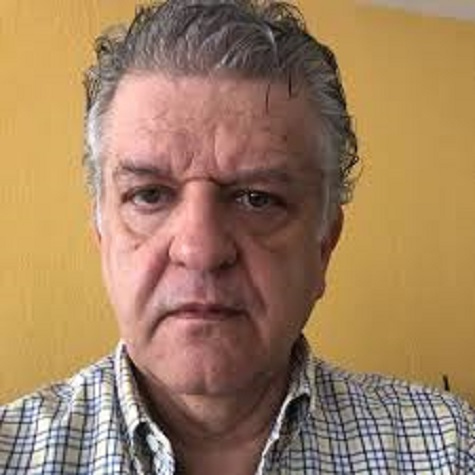
\includegraphics[width=1.36458in,height=\textheight]{images/belmiro_do_nascimento_joao-2.jpg}

\begin{quote}
\textbf{Dados} \emph{são sequências de fatos ainda não analisados, antes de serem organizados e ar­ ranjados de um jeito que as pessoas possam compreendê-los.} (João, Belmiro Nascimento - 2017)
\end{quote}

\begin{quote}
\textbf{Informação} \emph{é um dado organizado e apresentado de forma útil.} (João, Belmiro Nascimento - 2017)
\end{quote}

\begin{quote}
\textbf{Conhecimento} é o resultado da aplicação da informação para tomada de decisão. (João, Belmiro Nascimento - 2017)
\end{quote}

Exemplo de \textbf{Dados} versus \textbf{Informação}:

As caixas dos supermercados registram milhões de dados, como o código de barras dos produtos. Se somarmos e analisarmos esses dados, pode­ mos obter informações significativas, como o número total de detergentes vendidos em uma loja ou as vendas por região.

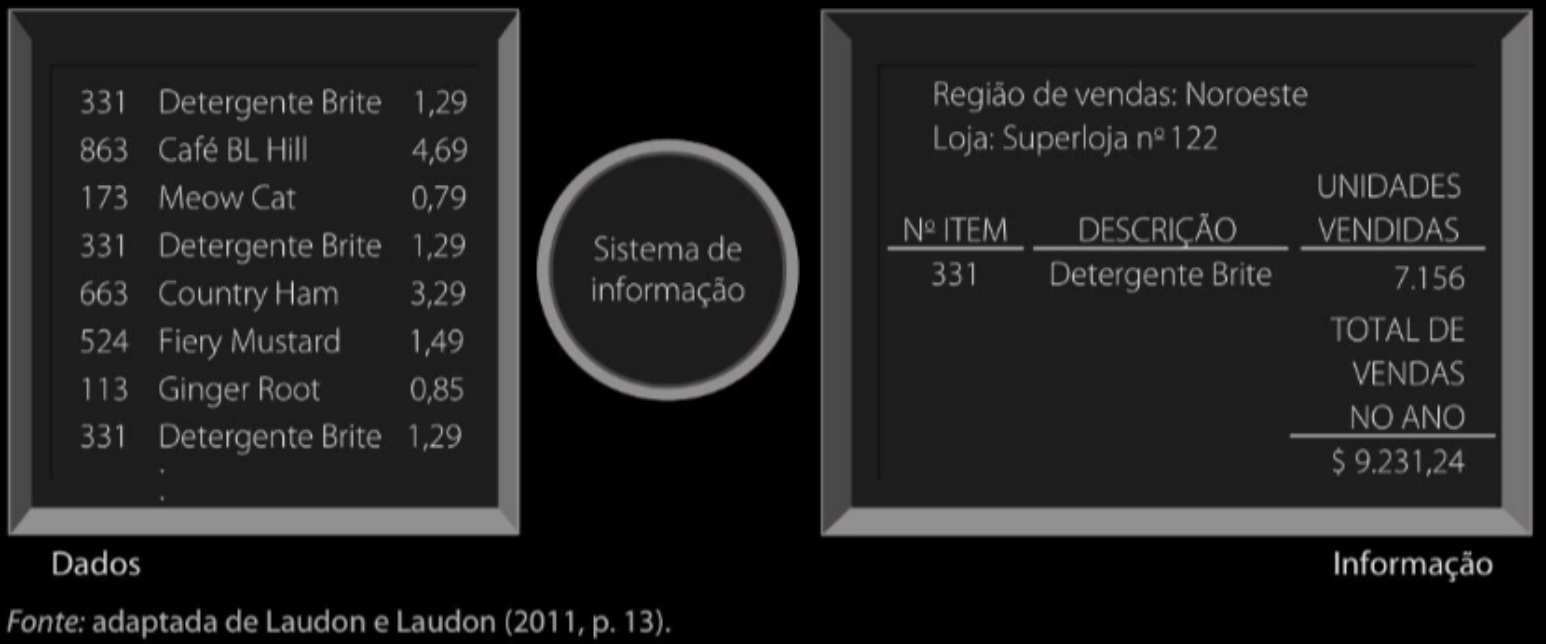
\includegraphics{images/1-dados-info/Dados-Info.jpg}

Fonte: LAUDON E LAUDON (2011, Pág 13)

\subsubsection{\texorpdfstring{Conceito de TIC -Tecnologia da informação e Comunicação \textbf{segundo} \emph{Kenneth C. LAUDON, Jane P. LAUDON} (2011)}{Conceito de TIC -Tecnologia da informação e Comunicação segundo Kenneth C. LAUDON, Jane P. LAUDON (2011)}}\label{conceito-de-tic--tecnologia-da-informauxe7uxe3o-e-comunicauxe7uxe3o-segundo-kenneth-c.-laudon-jane-p.-laudon-2011}

\begin{quote}
As \textbf{Tecnologias da Informação e Comunicação} (TICs) são um \textbf{CONJUNTO de tecnologias} que combinam:

\textbf{Tecnologia da Informação (TI)}: Refere-se ao hardware, software e redes necessários para processar, armazenar e distribuir dados e informações;

\textbf{Tecnologia da Comunicação}: Inclui as tecnologias que facilitam a comunicação e o compartilhamento de informações, como redes de telecomunicações, internet e dispositivos móveis.
\end{quote}

\subsubsection{\texorpdfstring{Conceito de Sistemas de Informação (SI) segundo \emph{Kenneth C. LAUDON, Jane P. LAUDON} (2011)}{Conceito de Sistemas de Informação (SI) segundo Kenneth C. LAUDON, Jane P. LAUDON (2011)}}\label{conceito-de-sistemas-de-informauxe7uxe3o-si-segundo-kenneth-c.-laudon-jane-p.-laudon-2011}

\begin{figure}
\centering
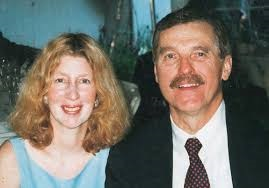
\includegraphics{images/Ken_Jane.jpg}
\caption{Prof Ken C. Laudon (1944 - 2019) e Jane Price Laudon - Universidade Columbia}
\end{figure}

\begin{quote}
\emph{``Tecnicamente, um \textbf{sistema de informação (Si)} é um CONJUNTO DE COMPONENTES RELACIONADOS entre si que COLETAM (ou recuperam), PROCESSAM, ARMAZENAM c DISTRIBUEM {[}o que ?{]} INFORMAÇÕES que servem para apoiar a TOMADA DE DECISÕES, a COORDENAÇÃO e o CONTROLE de uma organização.'' (LAUDON; LAUDON, 2011)}
\end{quote}

PERGUNTA: \emph{Um \textbf{SISTEMA DE INFORMAÇÃO (SI)} é a mesma coisa que um \textbf{computador (smartphone) com um software (app)}}?

a ) sim ? Porque ?\_\_\_\_\_\_\_\_\_\_\_\_\_\_\_\_\_\_\_\_\_\_\_\_\_\_\_\_\_\_\_\_\_\_\_\_\_\_\_\_\_\_\_\_\_\_\_\_\_\_\_\_\_\_\_\_\_\_\_\_\_\_\_\_\_\_\_\_\_\_\_\_\_\_\_\_\_\_\_\_\_\_\_\_\_\_\_\_\_

\begin{enumerate}
\def\labelenumi{\alph{enumi})}
\setcounter{enumi}{1}
\tightlist
\item
  nâo ? Porque ?\_\_\_\_\_\_\_\_\_\_\_\_\_\_\_\_\_\_\_\_\_\_\_\_\_\_\_\_\_\_\_\_\_\_\_\_\_\_\_\_\_\_\_\_\_\_\_\_\_\_\_\_\_\_\_\_\_\_\_\_\_\_\_\_\_\_\_\_\_\_\_\_\_\_\_\_\_\_\_\_\_\_\_\_\_\_\_\_\_
\end{enumerate}

\subsection{As 3 atividades básicas de um Sistema de Informação (SI)}\label{as-3-atividades-buxe1sicas-de-um-sistema-de-informauxe7uxe3o-si}

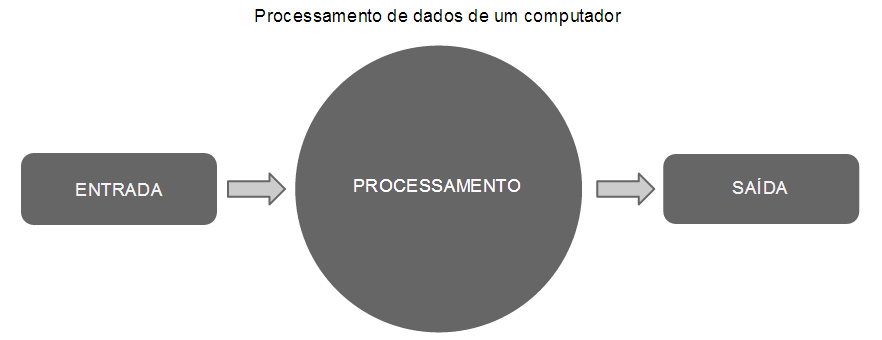
\includegraphics{images/processamento-dados-computador.png}

\subsection{Os Sistemas de Informação e o Mundo dos Negócios}\label{os-sistemas-de-informauxe7uxe3o-e-o-mundo-dos-neguxf3cios}

Em uma visão global, segundo JOAO, BELMIRO NASCIMENTO (2018) os Sistemas de Informação dentro das organizações são

\begin{quote}
soluções para vários problemas e desafios organizacionais. Essa abordagem tem relevância direta para sua carreira, pois \textbf{seus futu­ros empregadores contratarão você por sua habilidade em resolver problemas e atingir objetivos}.(JOÃO, BELMIRO NASCIMENTO - 2018)
\end{quote}

\subsection{A abordagem da resolução de problemas organizacionais}\label{a-abordagem-da-resoluuxe7uxe3o-de-problemas-organizacionais}

No mundo dos negócios as demandas (ou problemas) podem ser agrupados em 3 categorias:

\begin{itemize}
\item
  organização;
\item
  tecnologia;
\item
  pessoas;
\end{itemize}

Segundo \emph{Kenneth C. LAUDON, Jane P. LAUDON,} solucionar probelmas será sempre um processo contínuo de 4 passos:

\begin{enumerate}
\def\labelenumi{\arabic{enumi}.}
\item
  Identificar {[}do problema ou demanda{]};
\item
  Receber as propostas para Solução {[}do problema ou demanda{]};
\item
  Avaliar as propostas e escolher a Solução {[}do problema ou demanda{]};
\item
  Implantar a SOLUÇÂO escolhida {[}para resolver o problema ou demanda{]};
\end{enumerate}

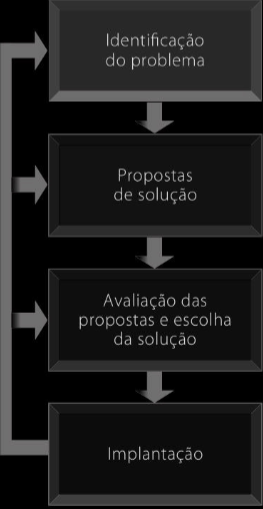
\includegraphics{images/clipboard-3657052893.png}

\begin{longtable}[]{@{}
  >{\raggedright\arraybackslash}p{(\columnwidth - 2\tabcolsep) * \real{0.3625}}
  >{\raggedright\arraybackslash}p{(\columnwidth - 2\tabcolsep) * \real{0.6375}}@{}}
\toprule\noalign{}
\begin{minipage}[b]{\linewidth}\raggedright
Os 4 passos para solucionar problemas (LAUDON e LAUDON)
\end{minipage} & \begin{minipage}[b]{\linewidth}\raggedright
Detalhes
\end{minipage} \\
\midrule\noalign{}
\endhead
\bottomrule\noalign{}
\endlastfoot
1- Identificar {[}problema ou demanda{]} & \begin{minipage}[t]{\linewidth}\raggedright
\begin{itemize}
\item
  Como resolver um problema que não sabemos qual é?
\item
  Os problemas precisam ser definidos pelas pessoas em uma orga­nização antes de serem resolvidos.
\end{itemize}
\end{minipage} \\
2- Propor Solução {[}problema ou demanda{]} & \begin{minipage}[t]{\linewidth}\raggedright
\begin{itemize}
\item
  Identificar soluções viáveis; Custo
\item
  Evitar ``bazuca para matar um pardal'';
\item
  Usar tecnologia ou usar melhor o ``recurso humano'' ?
\end{itemize}
\end{minipage} \\
3- Avaliar Propostas {[}problema ou demanda{]} & \begin{minipage}[t]{\linewidth}\raggedright
\begin{itemize}
\tightlist
\item
  Eficiência vs Eficácia !
\end{itemize}
\end{minipage} \\
4- Implantação {[}problema ou demanda{]} & \begin{minipage}[t]{\linewidth}\raggedright
\begin{itemize}
\tightlist
\item
  Qual a melhor solução ? Geralmente aquela que atende e é mais fácil de ser implantada;
\end{itemize}
\end{minipage} \\
\end{longtable}

\section{Os diferentes Tipos de Sistemas de Informação}\label{os-diferentes-tipos-de-sistemas-de-informauxe7uxe3o}

\textbf{Empresa existe para} (\textbf{cumprir seu propósito} que geralmente é) \textbf{DAR LUCRO} !

\subsubsection{Organizações com fins lucrativos - Empresas}\label{organizauxe7uxf5es-com-fins-lucrativos---empresas}

Uma empresa é uma organização formal cujo ob­ jetivo é produzir produtos ou prestar serviços a fim de obter lu­ cro. E como obter lucro? A conta é simples: vendem-se produtos a um preço superior aos custos da produção.

\subsubsection{Organizações sem fins lucrativos - Fundações Autarquicas - ONGs - Assitência Social - Saúde - Educação - Cultura - Direitos Humanos}\label{organizauxe7uxf5es-sem-fins-lucrativos---fundauxe7uxf5es-autarquicas---ongs---assituxeancia-social---sauxfade---educauxe7uxe3o---cultura---direitos-humanos}

As entidades sem fins lucrativos (dentre as quais estão ONGs ) são organizações que têm como objetivo principal promover o bem-estar social, defender causas ou oferecer serviços à comunidade, sem visar lucro financeiro.

\subsubsection{Organograma de uma Empresa: Uma Representação Visual da Estrutura Organizacional}\label{organograma-de-uma-empresa-uma-representauxe7uxe3o-visual-da-estrutura-organizacional}

Um organograma é uma representação gráfica da estrutura interna de uma organização, mostrando a hierarquia, os cargos, as funções e os departamentos que a compõem. Ele serve como um \textbf{mapa visual} da organização, facilitando a compreensão de \textbf{como as diferentes partes se encaixam} e como o \textbf{poder e a responsabilidade são distribuídos}.

\subsubsection{Organograma Conceitual}\label{organograma-conceitual}

\includegraphics{images/organogramas/organograma-genérico.jpg}

\textbf{Organograma Empresarial - Varejo}

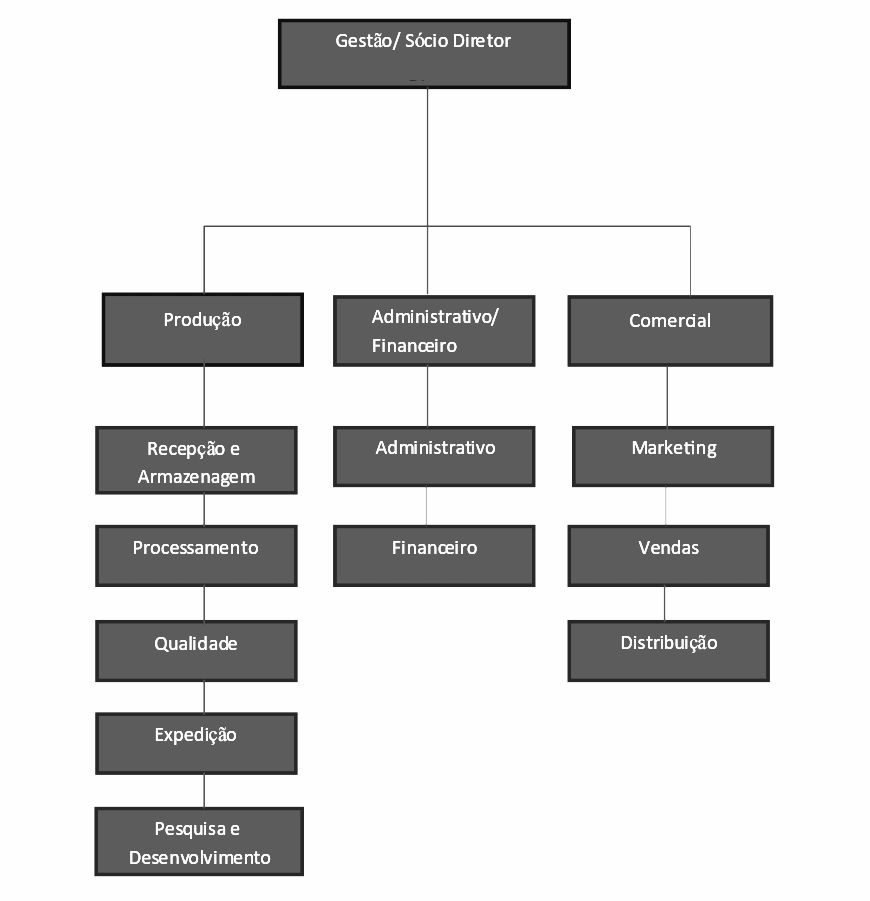
\includegraphics{images/organogramas/Organograma-empresarial.jpg}

\textbf{Organograma Empresarial - Indústria}

Aparece uma ``organela'' responsável por PRODUÇÃO

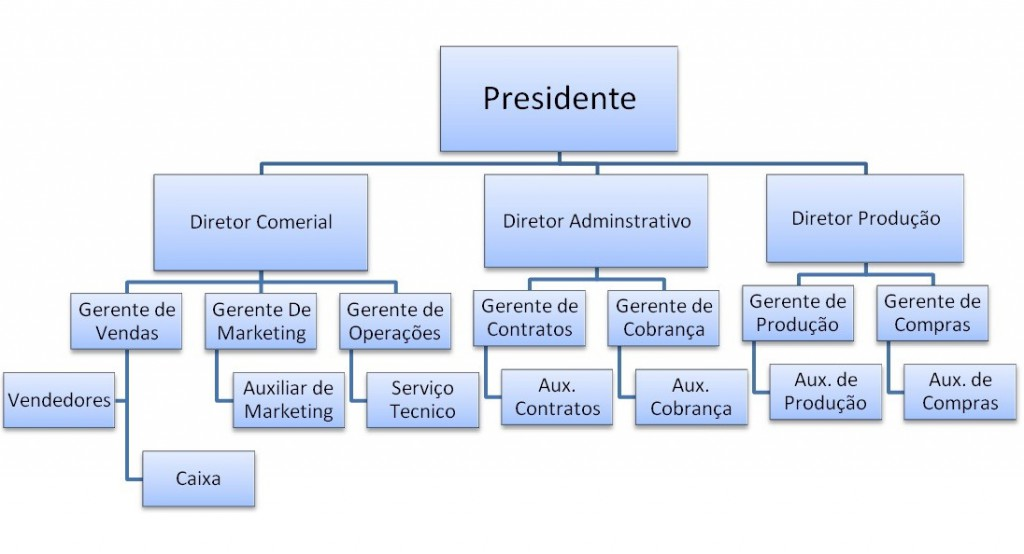
\includegraphics{images/organogramas/OrganogramaIndustrial.jpg}

\textbf{Organograma Organizacional - Organização Sem Fins Lucrativos - Orgão Público}

Exemplo: organograma da Superintendência Estadual de São Paulo do IBGE - Fundação pública da esfera do Poder Executivo Federal

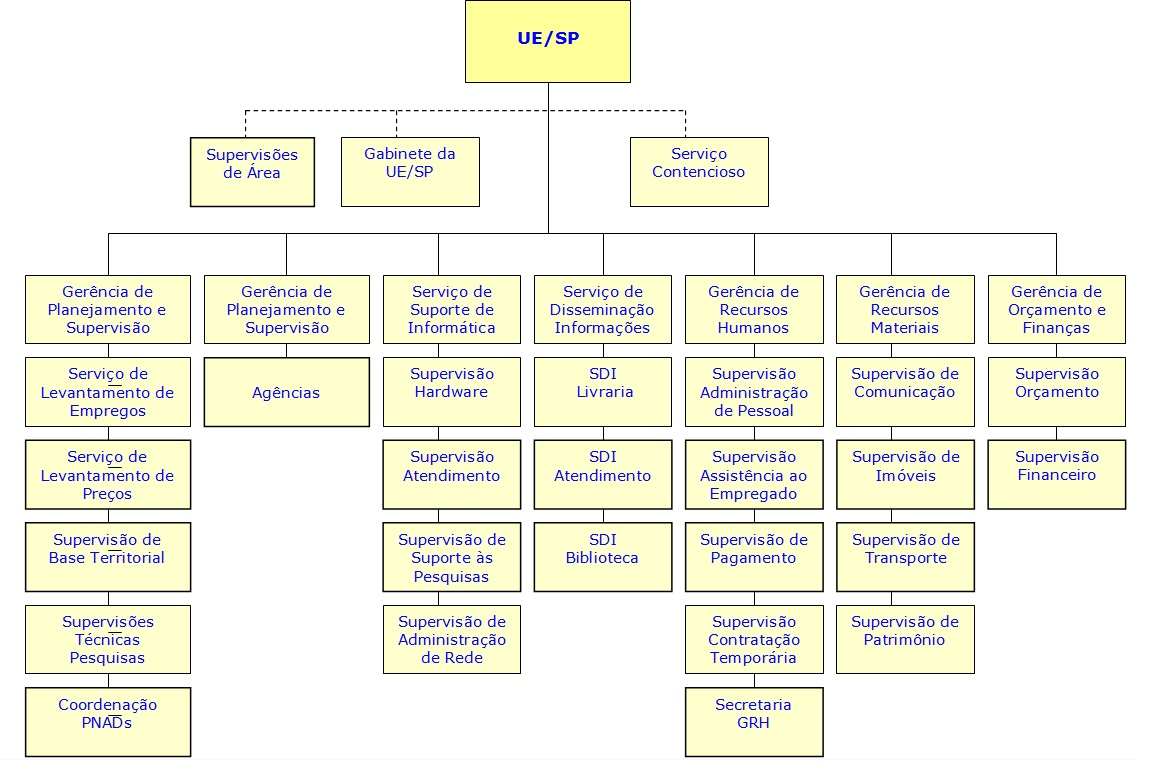
\includegraphics{images/organogramas/SES-SP.jpg}

\textbf{Missão} institucional dessa ``organização'' federal ``\emph{Retratar o Brasil com informações necessárias ao conhecimento de sua realidade e ao exercício da cidadania}''

\subsection{Organizando uma organização tipo empresa: funções empresariais básicas}\label{organizando-uma-organizauxe7uxe3o-tipo-empresa-funuxe7uxf5es-empresariais-buxe1sicas}

Imagine que você queira abrir seu próprio negócio. Você preci­ sará tomar várias decisões: o que produzir ou qual serviço prestar. Essa é uma escolha estratégica, pois vai determinar seus prováveis consumidores, os funcionários de que precisa, os métodos de pro­ dução c muitos outros aspectos. Depois de decidir o que produzir, você deve definir de que tipo de organização vai necessitar. Primeiro, pense em um arranjo de pessoas, máquinas c processos de negócios capaz de produzir. Em segundo lugar, monte uma equipe de marketing e vendas capaz de atrair clientes e vender o produto. Em terceiro, após as vendas, é preciso organizar uma equipe de contabilidade e finanças para cuidar das transações financeiras correntes, como pedidos, faturas e folhas de pagamento. Calma, ainda não acabou: também são necessárias pessoas para cuidar dos assuntos relativos aos funcio­ nários, como recrutamento e capacitação.

Essas quatro funções básicas - que você poderá ver na figura abaixo são encontradas em qualquer empresa. A figura também ajuda a identificar as princi­ pais entidades que formam uma empresa: fornecedores, clientes, funcionários, os salários que ela paga e, é claro, os produtos e serviços que produz.

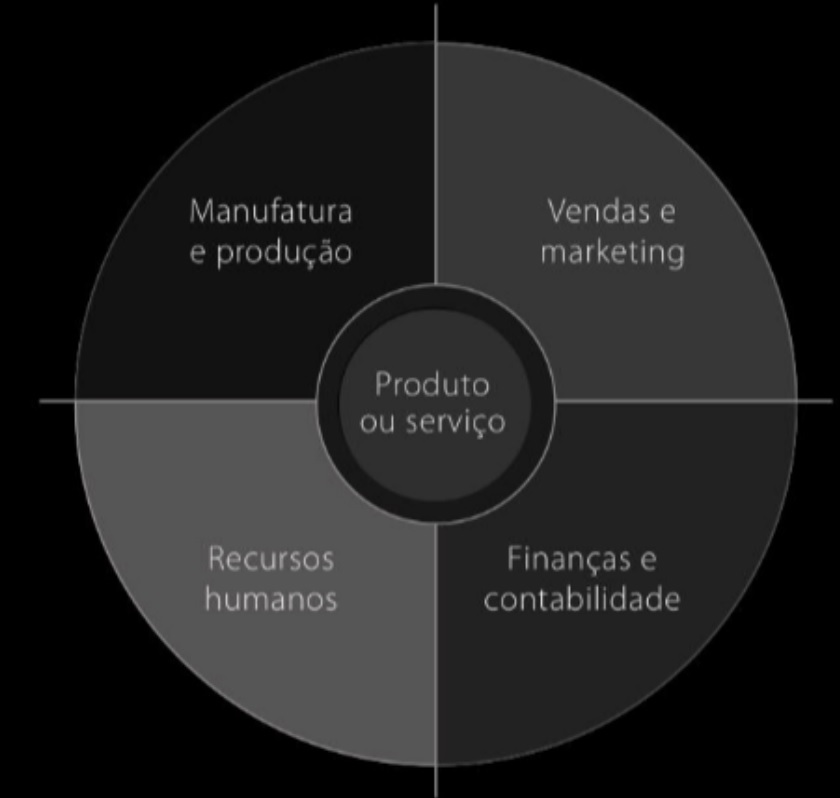
\includegraphics{images/1-dados-info/AreasBasicasEmpresa.jpg}

Fonte: adaptada de Laudon e Laudon (2011, página 37).

\begin{quote}
Organização -\textgreater{} Conhecimento do Negócio -\textgreater{} Processos Mapeados -\textgreater{} Sistema de Informação Mapeado
\end{quote}

\includegraphics{images/1-dados-info/ProcessosNegócioMapeados.jpg}

Processos do Cliclo de Vida da Produção de um produto (Indústria)

\section{Sistemas de Informação e Vantagem Competitiva}\label{sistemas-de-informauxe7uxe3o-e-vantagem-competitiva}

As empresas que se destacam em seus setores geralmente possuem algum tipo de \texttt{vantagem\ competitiva}.

As vantagens competitivas podem vir de dois aspectos a seguir:

\begin{itemize}
\item
  \textbf{recursos especiais};
\item
  \textbf{uso mais eficiente desses recursos};
\end{itemize}

\begin{longtable}[]{@{}
  >{\raggedright\arraybackslash}p{(\columnwidth - 6\tabcolsep) * \real{0.6667}}
  >{\centering\arraybackslash}p{(\columnwidth - 6\tabcolsep) * \real{0.1042}}
  >{\centering\arraybackslash}p{(\columnwidth - 6\tabcolsep) * \real{0.1042}}
  >{\centering\arraybackslash}p{(\columnwidth - 6\tabcolsep) * \real{0.1042}}@{}}
\toprule\noalign{}
\begin{minipage}[b]{\linewidth}\raggedright
Vantagem / Sistemas de Informação
\end{minipage} & \begin{minipage}[b]{\linewidth}\centering
SI ERP
\end{minipage} & \begin{minipage}[b]{\linewidth}\centering
SI SCM
\end{minipage} & \begin{minipage}[b]{\linewidth}\centering
SI CRM
\end{minipage} \\
\midrule\noalign{}
\endhead
\bottomrule\noalign{}
\endlastfoot
\textbf{Excelência operacional;} & ALTA & ALTA & ALTA \\
\textbf{Novos produtos, serviços e modelos de negócios;} & MÉDIA & SIM & SIM \\
\textbf{Relacionamento mais estreito com clientes e fornecedores;} & MÉDIA & ALTA & ALTA \\
\textbf{Melhor tomada de decisões;} & EXTREMA & ALTA & ALTA \\
\textbf{Sobrevivência no mercado;} & ALTA & ALTA & ALTA \\
\end{longtable}

\section{Tipos de sistemas de informação empresariais}\label{tipos-de-sistemas-de-informauxe7uxe3o-empresariais}

\begin{enumerate}
\def\labelenumi{\arabic{enumi}.}
\item
  \texttt{Sistemas\ de\ processamento\ de\ transações\ (SPTs)}; Monitoramento de pedidos de expedição de mercadoria; Monitoramento de pedidos de atendimento;
\item
  \texttt{Sistemas\ de\ informações\ gerenciais\ (SIGs)}; Relatório de faltas de funcionário; Relatório de mercadorias com defeito;
\item
  \texttt{Sistemas\ de\ apoio\ à\ decisão\ (SADs)}; Sistemas Business Inteligence;
\item
  \texttt{Sistemas\ de\ apoio\ ao\ executivo\ (SAEs)}; Relatório de vendas consolidado aos acionistas; Relatório de competitividade;
\item
  \textbf{Sistemas integrados (ERP);} Gestão e colaboração departamentos;
\item
  \textbf{Sistemas de gestão da cadeia de suprimentos (SCM);} Monitoramento de entrega de vendas on-line; Monitoramento Drop-Shipping;
\item
  \textbf{Sistemas de gestão do relacionamento com o cliente (CRM);} Relatório de satisfação de clientes; Relatório de Retenção de Clientes;
\item
  \textbf{Sistemas de gestão do conhecimento (SGCs);} Sistemas ITL; Sistemas de prestação de suporte técnico;
\end{enumerate}

\subsection{Sistemas integrados (E.R.P. - Planejamento de Recursos Empresariais ou Enterprise Resource Planning )}\label{sistemas-integrados-e.r.p.---planejamento-de-recursos-empresariais-ou-enterprise-resource-planning}

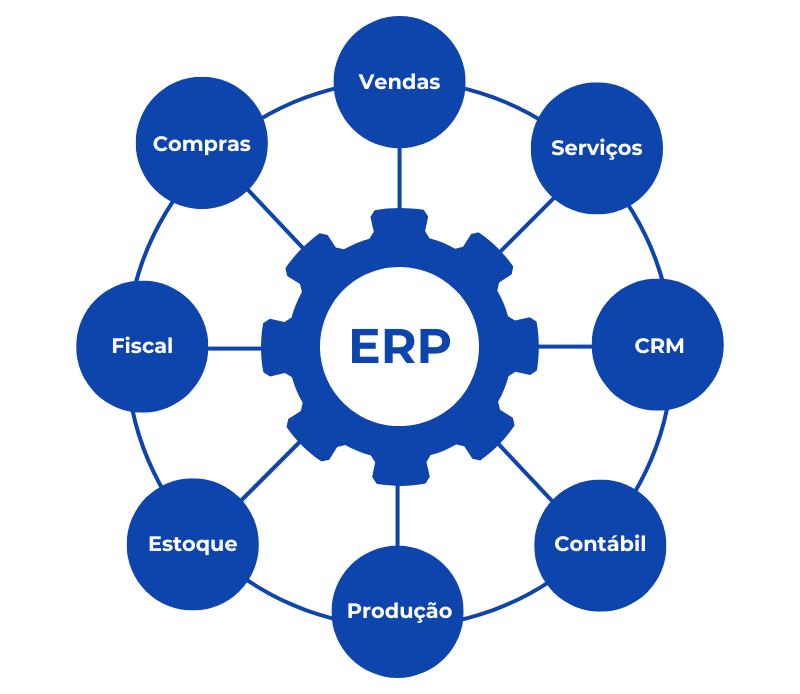
\includegraphics[width=6.28125in,height=\textheight]{images/sistemas/erp.png}

O termo ERP foi cunhado pelo Gartner Group em 1990. Um sistema ERP, segundo Davenport (1998)

\begin{quote}
'' \textbf{\emph{ERP é um sistema de software que integra todas as áreas funcionais de uma empresa, desde finanças e contabilidade até produção e vendas.}} '' Davenport, T. H. (1998). Putting the enterprise into the enterprise system. Harvard business review, 76(4), 121-131.
\end{quote}

As principais funções de um sistema ERP em empresas do varejo são:

\begin{itemize}
\item
  Centralizar a gestão operacional
\item
  Gerir o estoque e os suprimentos
\item
  Emitir notas fiscais
\item
  Controlar as finanças
\item
  Cadastrar clientes e produtos
\item
  Administrar a empresa
\end{itemize}

Alguns exemplos de SIs ERPs, em 2025, são:

\begin{itemize}
\item
  Pacote \href{https://www.sap.com/brazil/products/erp.html}{SAP ERP};
\item
  Pacote \href{https://www.oracle.com/br/erp/}{Oracle ERP Cloud};
\item
  Pacote \href{https://www.microsoft.com/pt-br/dynamics-365/pricing-overview}{Microsoft Dynamics 365};
\item
  Pacote \href{https://www.infor.com/pt-br}{Infor ERP};
\item
  Pacote \href{https://www.netsuite.com/portal/br/products/erp.shtml}{NetSuite ERP};
\item
  Sistema ERP \href{https://www.totvs.com/sistema-de-gestao/}{TOTVS};
\item
  Sistema ERP Web \href{https://www.bling.com.br/}{BLING};
\end{itemize}

\subsection{Sistemas de gestão da cadeia de suprimentos (supply chain management - SCM)}\label{sistemas-de-gestuxe3o-da-cadeia-de-suprimentos-supply-chain-management---scm}

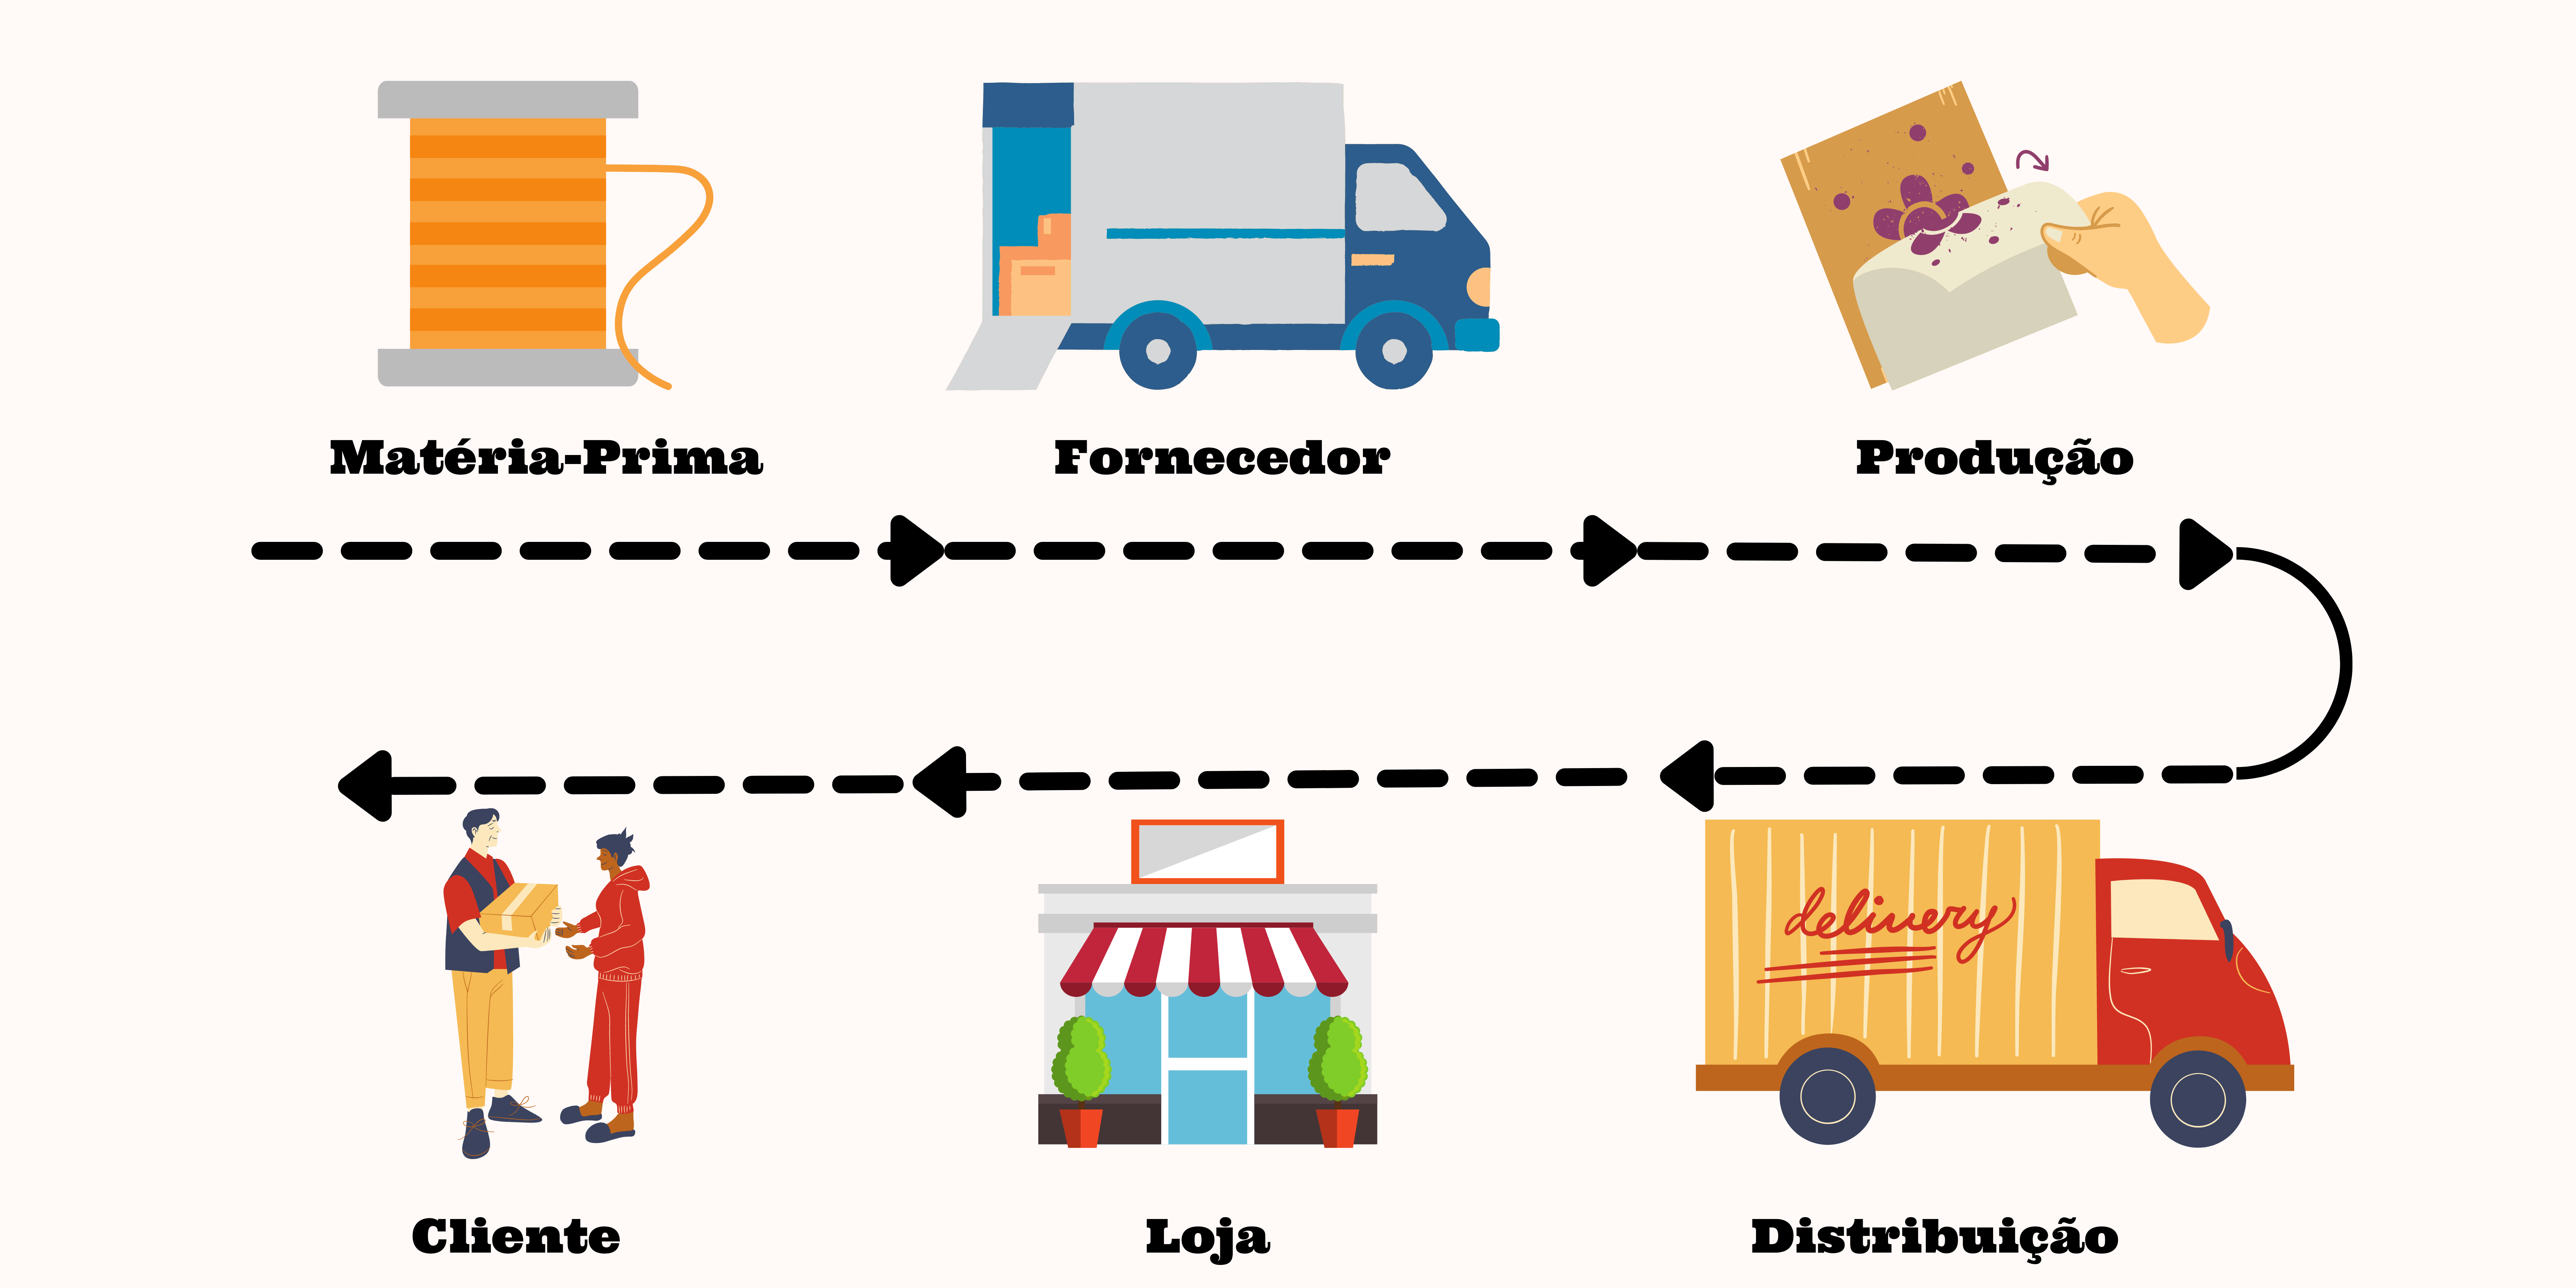
\includegraphics[width=7.4375in,height=\textheight]{images/sistemas/SCM.png}

Os SI SCM são ferramentas essenciais para otimizar o fluxo de produtos, informações e finanças desde a origem até o consumidor final. Eles abrangem todas as etapas da cadeia de suprimentos, desde a aquisição de matérias-primas até a entrega do produto final ao cliente.

Segundo Simchi-Levi, D., Kaminsky, P., \& Simchi-Levi, E. (2008)

\begin{quote}
\textbf{\emph{SCMé um SI que faz um conjunto de abordagens utilizadas para INTEGRAR eficientemente FORNECEDORES, ARMAZENS e LOJAS, de modo que as MERCADORIAS sejam PRODUZIDAS e DISTRIBUÍDAS nas QUANTIDADES certas, para os LOCAIS certos e nos MOMENTOS certos, a fim de MINIMIZAR os CUSTOS de todo o sistema, satisfazendo os requisitos de nível de serviço.}} Designing and managing the supply chain: concepts, strategies, and case studies de David Simchi-Levi, Philip Kaminsky e Edith Simchi-Levi. (2008)
\end{quote}

As principais funções de um SI SCM são:

\begin{itemize}
\item
  Reduzir custos: Otimizando processos, estoques e transportes.
\item
  Melhorar a eficiência: Agilizando o fluxo de produtos e informações.
\item
  Aumentar a satisfação do cliente: Garantindo entregas no prazo e produtos de qualidade.
\item
  Otimizar toda a cadeia de suprimentos: Interligando todas as etapas, desde fornecedores até clientes.
\end{itemize}

Alguns exemplos de SIs SCMs, em 2025, são:

\begin{itemize}
\item
  Oracle SCM Cloud;
\item
  SAP SCM;
\item
  Blue Yonder (JDA Software);
\end{itemize}

\subsection{Sistemas de Relacionamento com Cliente - CRM (Customer Relationship Management)}\label{sistemas-de-relacionamento-com-cliente---crm-customer-relationship-management}

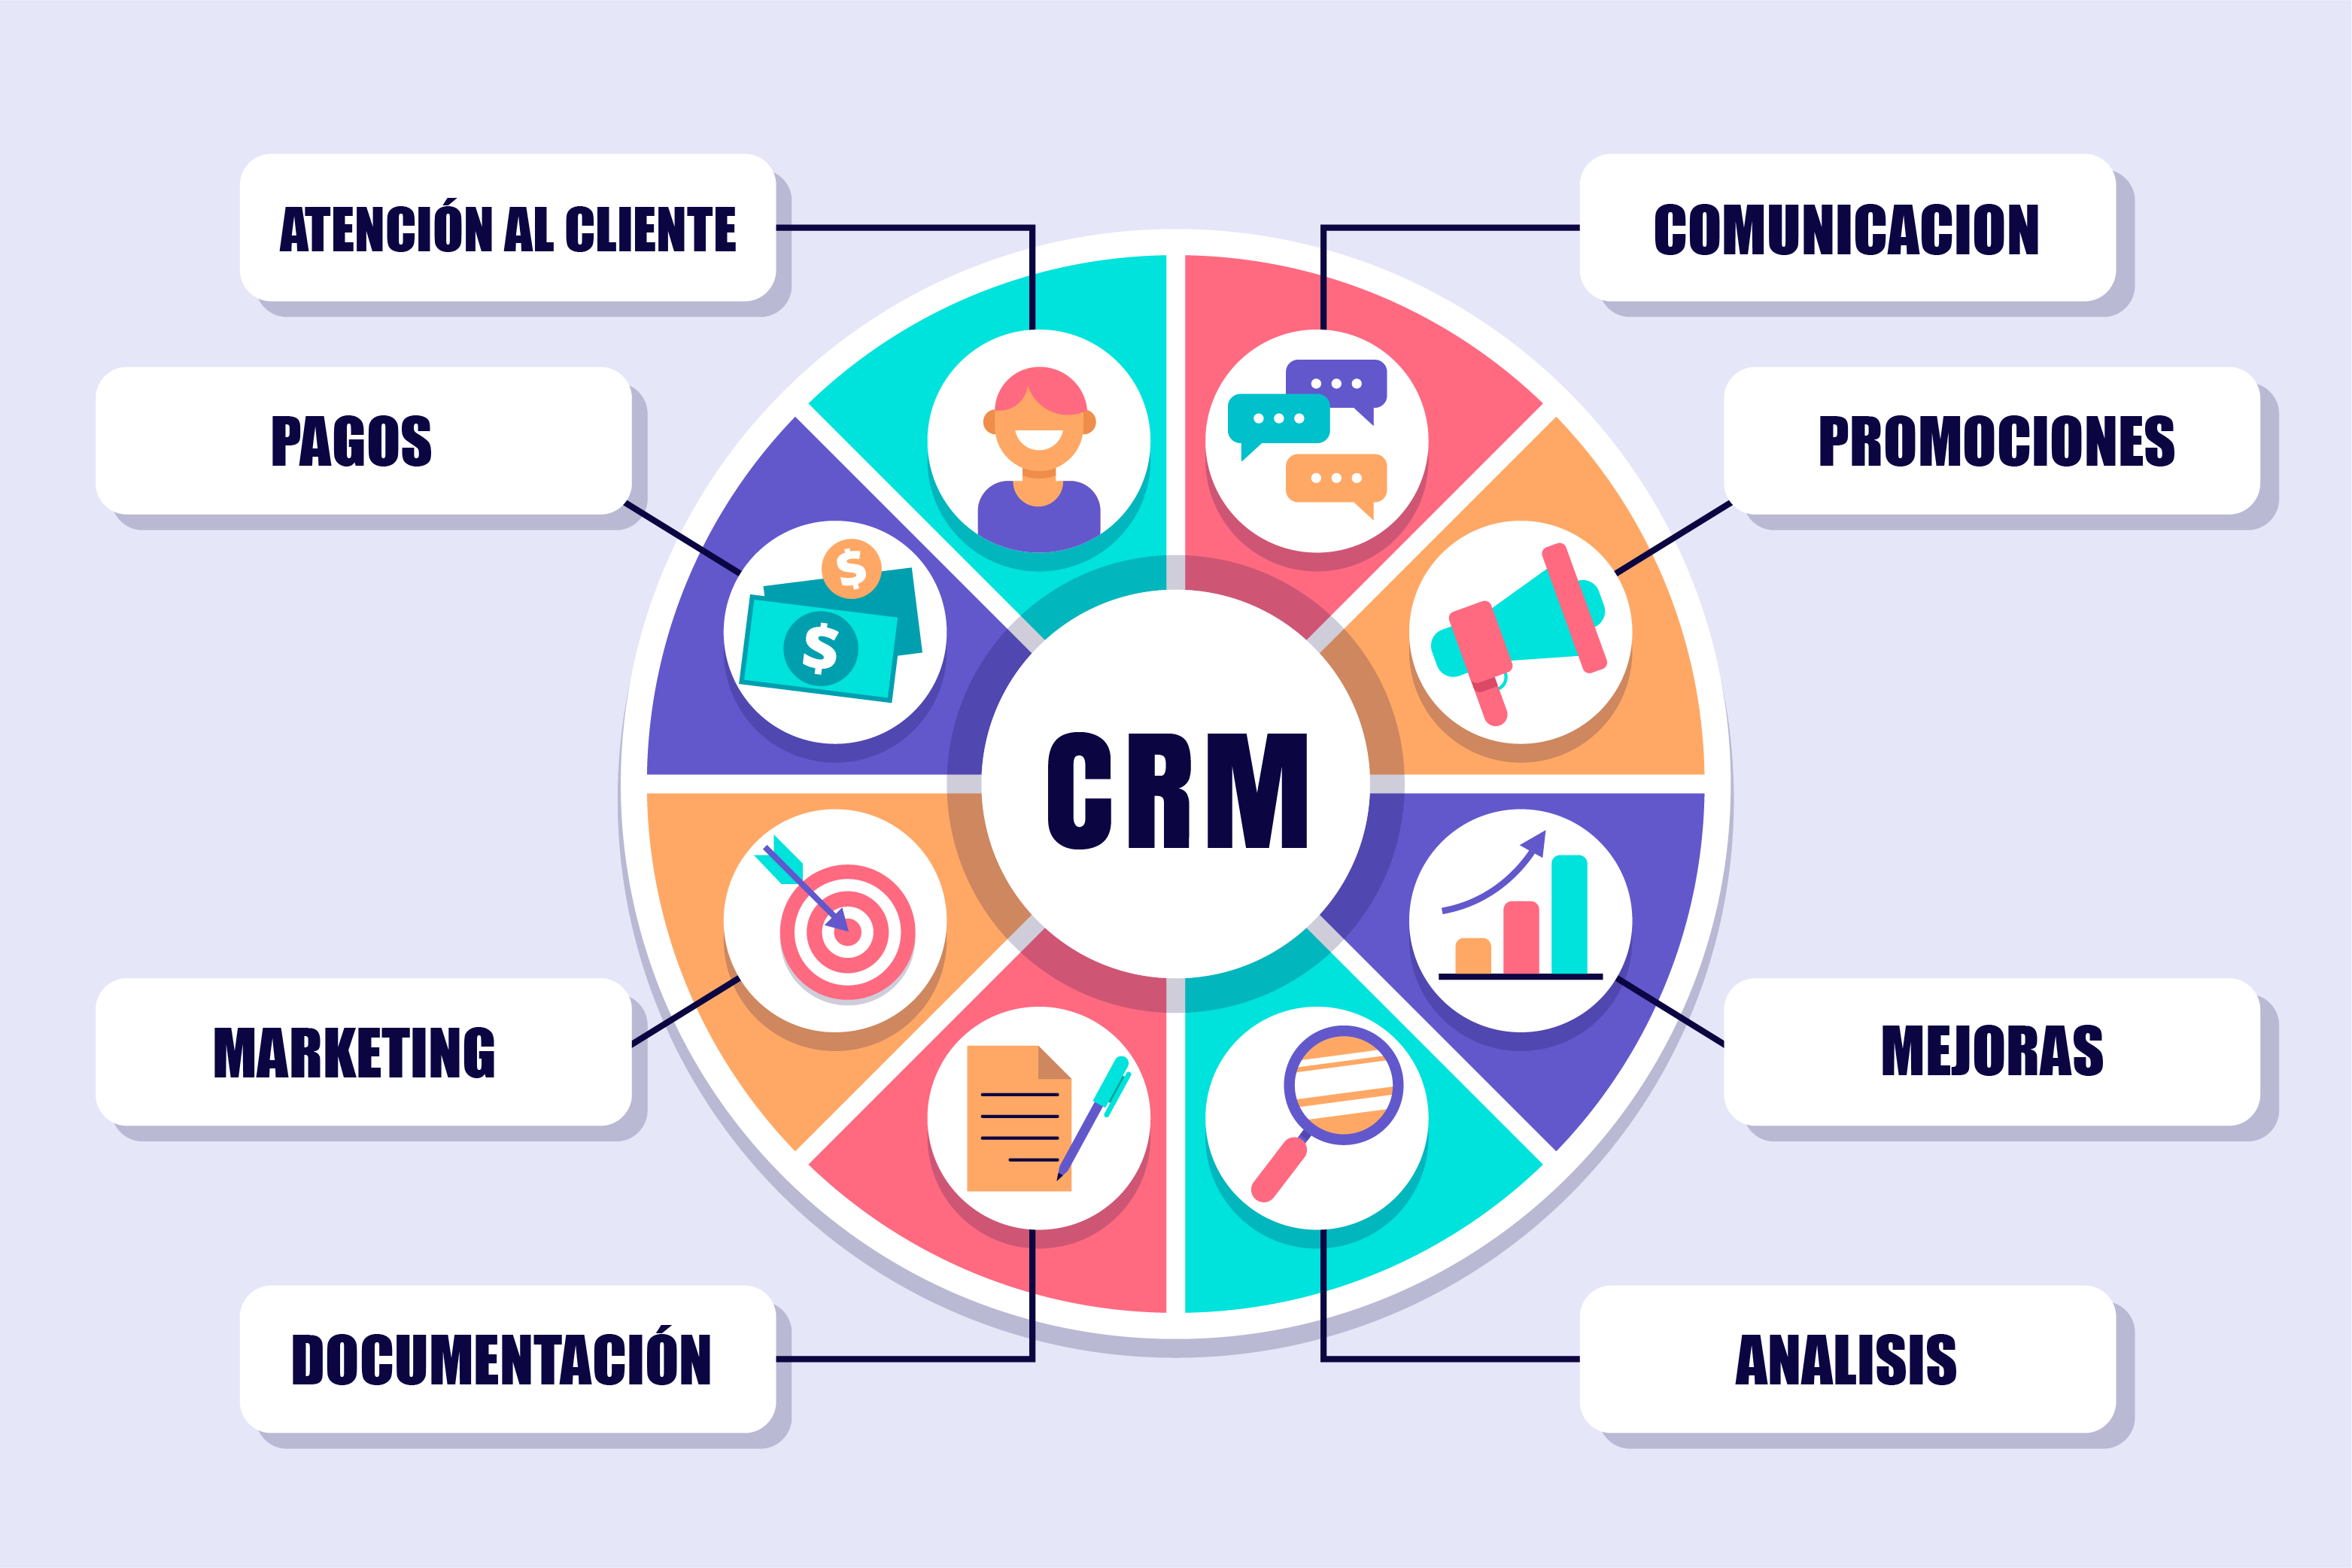
\includegraphics[width=6.6875in,height=\textheight]{images/sistemas/CRM.png}

São SIs de análise de clientes, com o objetivo de melhorar o relacionamento, aumentar a fidelização e impulsionar as vendas. Segundo Kotler, P., \& Keller, K. L. (2016), um um CRM pode ser definido assim

\begin{quote}
\textbf{\emph{Um SI CRM implanta o processo de gerenciar informações detalhadas sobre clientes individuais e gerenciar cuidadosamente todos os pontos de contato do cliente para maximizar a lealdade do cliente.}} Kotler, P., \& Keller, K. L. (2016). Marketing management
\end{quote}

As principais funções de um SI CRM são:

\begin{itemize}
\item
  Coleta e organização de dados: Reunindo informações sobre clientes, histórico de compras, interações e preferências.
\item
  Automação de processos: Otimizando tarefas de marketing, vendas e atendimento ao cliente.
\item
  Análise de dados: Identificando padrões e insights para melhorar a tomada de decisões.
\item
  Personalização do atendimento: Oferecendo experiências individualizadas aos clientes.
\end{itemize}

Alguns exemplos de SIs CRMs, em 2025, são:

\begin{itemize}
\item
  Salesforce CRM;
\item
  Microsoft Dynamics 365;
\item
  HubSpot CRM;
\item
  Zendesk Sell;
\end{itemize}

\section{Exercícios}\label{exercuxedcios}

\section{Questões}\label{questuxf5es}

\begin{enumerate}
\def\labelenumi{\arabic{enumi}.}
\item
  Qual o \textbf{papel dos sistemas de informação no ambiente de negócios contemporâneo}?
\item
  Quais são os \textbf{objetivos organizacionais dos sistemas de informação}?
\item
  Qual a \textbf{diferença entre dados e informações}?
\item
  Quais são as \textbf{atividades básicas em um sistema de informação}?
\item
  O que são \textbf{abordagens de resolução de problemas organizacionais} e como aplicá-las?
\item
  O que é uma \textbf{empresa} e quais os seus componentes?
\item
  Quais as \textbf{funções básicas de uma empresa}?
\item
  Quais os \textbf{níveis hierárquicos de uma empresa}?
\item
  Quais os \textbf{tipos de sistemas de informação empresariais}?
\item
  O que é \textbf{colaboração}?
\item
  Qual a \textbf{função dos sistemas de informação em uma empresa}?
\item
  Como usar os \textbf{sistemas de informação para conquistar vantagem competitiva}?
\end{enumerate}

\section{Testes múltipla escolha}\label{testes-muxfaltipla-escolha}

\textbf{1. Qual das seguintes alternativas descreve melhor o propósito e a função de um Sistema de Planejamento de Recursos Empresariais (ERP)?}

\begin{enumerate}
\def\labelenumi{\alph{enumi})}
\item
  Um sistema ERP é utilizado principalmente para gerenciar o relacionamento com os clientes, coletando e analisando dados de interações para melhorar as vendas e o atendimento ao cliente.
\item
  Um sistema ERP foca-se na gestão da cadeia de suprimentos, coordenando atividades entre fornecedores, fabricantes e distribuidores para otimizar o fluxo de produtos.
\item
  Um sistema ERP é projetado para capturar e aplicar conhecimento dentro da organização, facilitando a criação, o armazenamento e a transferência de expertise entre os funcionários.
\item
  Um sistema ERP integra processos de negócios em áreas como manufatura, finanças, vendas e recursos humanos em um único sistema de software, permitindo o acesso e o compartilhamento de informações em toda a organização.
\item
  Um sistema ERP serve para analisar dados históricos e atuais da empresa, a fim de identificar tendências de mercado e prever o comportamento do consumidor.
\end{enumerate}

\textbf{2. Qual das seguintes alternativas descreve melhor a função de um sistema de informação (SI) em uma empresa?}

\begin{enumerate}
\def\labelenumi{\alph{enumi})}
\item
  Um SI serve principalmente para gerenciar a cadeia de suprimentos, otimizando o fluxo de produtos desde os fornecedores até os clientes.
\item
  Um SI tem como principal função coletar dados brutos e não organizados sobre as operações da empresa.
\item
  Um SI é um conjunto de componentes relacionados que coletam, processam, armazenam e distribuem informações para apoiar a tomada de decisões, a coordenação e o controle da organização.
\item
  Um SI é usado para transformar dados em informações úteis, apresentando-os de forma organizada e compreensível.
\item
  Um SI é utilizado principalmente para integrar todos os processos de negócios da empresa em um único sistema de software, facilitando o acesso e o compartilhamento de dados.
\end{enumerate}

\section{Respostas questões:}\label{respostas-questuxf5es}

\begin{enumerate}
\def\labelenumi{\arabic{enumi}.}
\tightlist
\item
  Qual o \textbf{papel dos sistemas de informação no ambiente de negócios contemporâneo}?
\end{enumerate}

\textbf{Resposta}: Ajudar a atingir Objetivos organizacionais, promover a transformação do negócio, promover integração e colaboração das áreas, criar Vantagem competitiva e, finalmente, ajudar na tomada de decisões.

\begin{enumerate}
\def\labelenumi{\arabic{enumi}.}
\setcounter{enumi}{1}
\tightlist
\item
  Quais são os \textbf{objetivos organizacionais dos sistemas de informação}?
\end{enumerate}

\textbf{Resposta}: Promover excelência operacional, possibilitar novos produtos e modelos de negócio, ajudar o relacionamento entre clientes e fornecedores.

\begin{enumerate}
\def\labelenumi{\arabic{enumi}.}
\setcounter{enumi}{2}
\tightlist
\item
  Qual a \textbf{diferença entre dados e informações}?
\end{enumerate}

\textbf{Resposta}: Dados são sequência de informações ainda não analisados. Informações são dados apresentados de forma útil.

\begin{enumerate}
\def\labelenumi{\arabic{enumi}.}
\setcounter{enumi}{3}
\tightlist
\item
  Quais são as \textbf{atividades básicas em um sistema de informação}?
\end{enumerate}

\textbf{Resposta}: Entrada, Processamento e Saída.

\begin{enumerate}
\def\labelenumi{\arabic{enumi}.}
\setcounter{enumi}{4}
\tightlist
\item
  O que são \textbf{abordagens de resolução de problemas organizacionais} e como aplicá-las?
\end{enumerate}

\textbf{Resposta}: Identificar Problema, Propor Solução, Escolher Solução, Implantar Solução.

\begin{enumerate}
\def\labelenumi{\arabic{enumi}.}
\setcounter{enumi}{5}
\tightlist
\item
  O que é uma \textbf{empresa} e quais os seus componentes?
\end{enumerate}

\textbf{Resposta}: Uma empresa é uma organização formal cujo objetivo é produzir produtos ou prestar serviços a fim de obter lucro. Seus componentes são CLIENTES, FORNECEDORES, FUNCIONÁRIOS, PRODUTOS E SERVIÇOS.

\begin{enumerate}
\def\labelenumi{\arabic{enumi}.}
\setcounter{enumi}{6}
\tightlist
\item
  Quais as \textbf{funções básicas de uma empresa}?
\end{enumerate}

\textbf{Resposta}: Manufatura e produção, Vendas e marketing, Recursos humanos e; Finanças e Contabilidade.

\begin{enumerate}
\def\labelenumi{\arabic{enumi}.}
\setcounter{enumi}{8}
\tightlist
\item
  Quais os \textbf{níveis hierárquicos de uma empresa}?
\end{enumerate}

\textbf{Resposta}: Gerência sênior (Conselho Diretor e Presidente), Gerência média (Diretores), Gerência operacional (Gerentes), Trabalhadores do conhecimento (analistas setoriais), Trabalhadores de dados (analistas setoriais), Trabalhadores dos serviços ou da produção (chão-de-fábrica).

\begin{enumerate}
\def\labelenumi{\arabic{enumi}.}
\setcounter{enumi}{9}
\tightlist
\item
  Quais os \textbf{tipos de sistemas de informação empresariais}?
\end{enumerate}

\textbf{Resposta}: Sistemas integrados (ERP), Sistemas de gestão da cadeia de suprimentos (SCM), Sistemas de gestão do relacionamento com o cliente (CRM) e Sistemas de gestão do conhecimento (SGCs).

\begin{enumerate}
\def\labelenumi{\arabic{enumi}.}
\setcounter{enumi}{10}
\tightlist
\item
  O que é \textbf{colaboração}?
\end{enumerate}

\textbf{Resposta}: colaboração é o trabalho com os outros para alcançar metas claras e compartilhadas.

\begin{enumerate}
\def\labelenumi{\arabic{enumi}.}
\setcounter{enumi}{11}
\tightlist
\item
  Qual a \textbf{função dos sistemas de informação em uma empresa}?
\end{enumerate}

\textbf{Resposta}: Coletar (ou Recuper), Processar, Armazenar e distribuir INFORMAÇÕES.

\begin{enumerate}
\def\labelenumi{\arabic{enumi}.}
\setcounter{enumi}{12}
\tightlist
\item
  Como usar os \textbf{sistemas de informação para conquistar vantagem competitiva}?
\end{enumerate}

\textbf{Resposta}: Melhorando a gestão de processos de negócios.

\section{Respostas dos testes:}\label{respostas-dos-testes}

\begin{longtable}[]{@{}cc@{}}
\toprule\noalign{}
Questão & Resposta \\
\midrule\noalign{}
\endhead
\bottomrule\noalign{}
\endlastfoot
1 & D \\
2 & C \\
\end{longtable}

\chapter{NP1}\label{np1}

\section{Grupos até 2025-03-27}\label{grupos-atuxe9-2025-03-27}

\subsection{Turma Campus Chácara Santo Antônio}\label{turma-campus-chuxe1cara-santo-antuxf4nio}

\begin{longtable}[]{@{}
  >{\raggedright\arraybackslash}p{(\columnwidth - 12\tabcolsep) * \real{0.0450}}
  >{\raggedright\arraybackslash}p{(\columnwidth - 12\tabcolsep) * \real{0.2883}}
  >{\raggedright\arraybackslash}p{(\columnwidth - 12\tabcolsep) * \real{0.0901}}
  >{\raggedright\arraybackslash}p{(\columnwidth - 12\tabcolsep) * \real{0.0721}}
  >{\raggedright\arraybackslash}p{(\columnwidth - 12\tabcolsep) * \real{0.2252}}
  >{\raggedright\arraybackslash}p{(\columnwidth - 12\tabcolsep) * \real{0.1441}}
  >{\raggedright\arraybackslash}p{(\columnwidth - 12\tabcolsep) * \real{0.1351}}@{}}
\toprule\noalign{}
\begin{minipage}[b]{\linewidth}\raggedright
ID
\end{minipage} & \begin{minipage}[b]{\linewidth}\raggedright
Nome do Aluno
\end{minipage} & \begin{minipage}[b]{\linewidth}\raggedright
RA
\end{minipage} & \begin{minipage}[b]{\linewidth}\raggedright
Turma
\end{minipage} & \begin{minipage}[b]{\linewidth}\raggedright
GRUPO
\end{minipage} & \begin{minipage}[b]{\linewidth}\raggedright
NP1 -- Trabalho
\end{minipage} & \begin{minipage}[b]{\linewidth}\raggedright
NP1 -- Prática
\end{minipage} \\
\midrule\noalign{}
\endhead
\bottomrule\noalign{}
\endlastfoot
9 & CARLOS EDUARDO SILVA BATISTA & R448DE-8 & DS1P40 & GRUPO CONNECTI & & \\
95 & RAMON BRIAN GONÇALVES DOS SANT & R85236-9 & DS1Q40 & GRUPO CONNECTI & & \\
99 & RICHARD RODRIGUES MEDEIROS & H75556-5 & DS1Q40 & GRUPO CONNECTI & & \\
89 & PEDRO EDUARDO PAIVA MEIRELES & R8699H-4 & DS1Q40 & GRUPO CONNECTI & & \\
1 & ANDERSON RAULINO DA SILVA & F3620J-8 & DS1P40 & GRUPO CORETECH & & \\
18 & FREDSON SILVA DOS SANTOS & R427FB-0 & DS1P40 & GRUPO CORETECH & & \\
92 & PEDRO LEONILDO DA SILVA TEIXEI & R65838-4 & DS1Q40 & GRUPO CORETECH & & \\
12 & CAUAN NUNES LOPES & H6771G-9 & DS1P40 & GRUPO CWE & & \\
15 & EDER RODRIGUES DE ALMEIDA & R8459C-7 & DS1P40 & GRUPO CWE & & \\
78 & MATHEUS KAUÃ VERAS SANTORES & R8461B-7 & DS1Q40 & GRUPO CWE & & \\
112 & WILLIAM DA SILVA CARVALHO & H5963E-7 & DS1Q40 & GRUPO CWE & & \\
10 & CARLOS EDUARDO SILVA SANTANA & F362EF-1 & DS1P40 & GRUPO CYBER SEED & & \\
25 & GUSTAVO RODRIGUES OGNIBENE MIG & R692AG-0 & DS1P40 & GRUPO CYBER SEED & & \\
39 & LINCOLN GUILHERME SANT ANNA BA & H7501D-3 & DS1P40 & GRUPO CYBER SEED & & \\
106 & VICTOR FERREIRA DA S RIBEIRO & R851DI-0 & DS1Q40 & GRUPO CYBER SEED & & \\
50 & MATHEUS BRIGANTI DE OLIVEIRA & H74FGI-8 & DS1P40 & GRUPO DEV SQUAD & & \\
82 & MICHEL FARIAS DA SILVA & R6607C-2 & DS1Q40 & GRUPO DEV SQUAD & & \\
105 & THIAGO FERREIRA DIAS & R218BC-1 & DS1Q40 & GRUPO DEV SQUAD & & \\
28 & HENRIQUE BASTOS LAET & R671IG-1 & DS1P40 & GRUPO EDUSOFT SOLUTIONS & & \\
116 & CAIO CESAR BALBINO DA SILVA & R536FA-6 & TI1P40 & GRUPO GJLC ENTERPRISE & & \\
120 & GABRIEL ROQUE DOS SANTOS & R6607G-5 & TI1P40 & GRUPO GJLC ENTERPRISE & & \\
34 & JOÃO VICTOR RODRIGUES SILVA & R83238-4 & DS1P40 & GRUPO GJLC ENTERPRISE & & \\
69 & LUCAS FERNANDES FIGUEIREDO & H76688-5 & DS1Q40 & GRUPO GJLC ENTERPRISE & & \\
60 & EDUARDO DE SOUSA PEREIRA & H759CH-8 & DS1Q40 & GRUPO HELIUS HOME & & \\
77 & MATHEUS DA SILVA BRITO & R839DA-4 & DS1Q40 & GRUPO HELIUS HOME & & \\
83 & MIGUEL DOS SANTOS MENDES SITOM & R540EA-6 & DS1Q40 & GRUPO HELIUS HOME & & \\
3 & ARTUR HENRIQUE DE OLIVEIRA VIT & H750FH-2 & DS1P40 & GRUPO INFINITECH & & \\
49 & MARIA EDUARDA RODRIGUES ROMÃO & R512ED-7 & DS1P40 & GRUPO INFINITECH & & \\
84 & MIKAEL MACEDO DA SILVA & H671CE-9 & DS1Q40 & GRUPO INFINITECH & & \\
17 & FERNANDA CRISTINA DA SILVA & R603CJ-7 & DS1P40 & GRUPO INFINITECH & & \\
11 & CAUA HENRIQUE R DOS SANTOS & R434FI-4 & DS1P40 & GRUPO INOVATECH & & \\
35 & JOÃO VITOR FREITAS DE OLIVEIRA & H755HH-9 & DS1P40 & GRUPO INOVATECH & & \\
124 & KEVIN MACIEL RODRIGUES MACHADO & R7994J-6 & TI1P40 & GRUPO INOVATECH & & \\
127 & LUCAS SOUZA RODRIGUES & R837AA-0 & TI1P40 & GRUPO INOVATECH & & \\
128 & MARCOS PAULO CORDEIRO GOES & H71441-9 & TI1P40 & GRUPO INOVATECH & & \\
75 & MATHEUS BALIEIRO GONÇALVES & R8245A-4 & DS1Q40 & GRUPO INOVATECH & & \\
102 & TAYNARA NOGUEIRA DOS SANTOS & R8439J-1 & DS1Q40 & GRUPO INOVATECH & & \\
4 & BARBARA COSTA NASCIMENTO & H60306-4 & DS1P40 & GRUPO INTEGRATECH & & \\
5 & BRUNA MEDEIROS DE AGUIAR & R81554-4 & DS1P40 & GRUPO INTEGRATECH & & \\
57 & BRUNO ALVES DE SOUZA & R8662A-7 & DS1Q40 & GRUPO INTEGRATECH & & \\
23 & GUSTAVO RIBEIRO DA SILVA & R846HB-8 & DS1P40 & GRUPO INTEGRATECH & & \\
37 & KAREN DE SOUSA FARIA & R8522D-0 & DS1P40 & GRUPO INTEGRATECH & & \\
6 & BRUNA SILVA DOS SANTOS & H66289-3 & DS1P40 & GRUPO INVEST & & \\
118 & DOUGLAS VINICIUS M DOS SANTOS & H6094I-1 & TI1P40 & GRUPO INVEST & & \\
26 & HECTOR CASTRO DE OLIVEIRA & H7477C-8 & DS1P40 & GRUPO INVEST & & \\
48 & LUIZA NASCIMENTO DA CONCEIÇÃO & H66046-7 & DS1P40 & GRUPO INVEST & & \\
7 & BRUNO RODRIGUES DE ALMEIDA & R8414G-8 & DS1P40 & GRUPO LEGACY & & \\
24 & GUSTAVO RODRIGUES DE BARROS & R69362-7 & DS1P40 & GRUPO LEGACY & & \\
90 & PEDRO HENRIQUE DE P MEDEIROS & R8514D-9 & DS1Q40 & GRUPO LEGACY & & \\
129 & MARIA EDUARDA R MASCARENHAS & H6689G-8 & TI1P40 & GRUPO LEGACY & & \\
59 & DANILO SALGADO PERALTA RIBEIRO & R868GI-1 & DS1Q40 & GRUPO LOGIC LAB & & \\
61 & GABRIEL GONCALVES ZAGO & H75GHA-1 & DS1Q40 & GRUPO LOGIC LAB & & \\
46 & LUIS FERNANDO ANDRADE SANTOS & H71274-2 & DS1P40 & GRUPO LOGIC LAB & & \\
91 & PEDRO HENRIQUE FORNAZARI DE SO & R82651-1 & DS1Q40 & GRUPO LOGIC LAB & & \\
56 & BRENO BRITO ALMEIDA & H76859-4 & DS1Q40 & GRUPO MINOS BUSINESS & & \\
80 & MATHEUS RENATO & R864CB-0 & DS1Q40 & GRUPO MINOS BUSINESS & & \\
100 & RONALDO C DE GOIS RAMOS & R533FB-5 & DS1Q40 & GRUPO MINOS BUSINESS & & \\
38 & LEONARDO ARAUJO FREIRES & R659EI-9 & DS1P40 & GRUPO NEW TIME & & \\
109 & VITOR ALEXANDRE DE JESUS AMORI & H66EIH-4 & DS1Q40 & GRUPO NEW TIME & & \\
32 & JOAO PEDRO SILVA CARVALHO & N001AE-7 & DS1P40 & GRUPO NEXTCON & & \\
51 & MAYSA PONT LOPES & T160GF-8 & DS1P40 & GRUPO NEXTCON & & \\
111 & VITÓRIA DE OLIVEIRA VITOR & R503IE-5 & DS1Q40 & GRUPO NEXTCON & & \\
31 & JERFFERSON DE SOUZA NASCIMENTO & H47127-3 & DS1P40 & GRUPO OFFICE SOLUTIONS & & \\
131 & RAMON BORGES DE HOLANDA & R85412-4 & TI1P40 & GRUPO OFFICE SOLUTIONS & & \\
96 & RAMON SANTOS SILVA & H75161-6 & DS1Q40 & GRUPO OFFICE SOLUTIONS & & \\
108 & VINICIUS FRANCA GARCIA DA CRUZ & H7584H-9 & DS1Q40 & GRUPO OFFICE SOLUTIONS & & \\
13 & CLEYTON ALVES DA COSTA & G77AIA-8 & DS1P40 & GRUPO QUANTUM SOLUTIONS & & \\
40 & LORRANY SILVA AMORIM & G71CJI-0 & DS1P40 & GRUPO QUANTUM SOLUTIONS & & \\
104 & THAMYRES BANDEIRA SANTOS & H6882F-0 & DS1Q40 & GRUPO QUANTUM SOLUTIONS & & \\
113 & YEDA GOMES DOS SANTOS CUSTODIO & R87269-6 & DS1Q40 & GRUPO QUANTUM SOLUTIONS & & \\
8 & CAIO CAVALCANTE BRITO & H50DJE-3 & DS1P40 & GRUPO SERVERP & & \\
14 & DAVID GABRIEL SILVA DE JESUS & F361DG-6 & DS1P40 & GRUPO SERVERP & & \\
43 & LUCAS PEREIRA SILVA & R84302-5 & DS1P40 & GRUPO SERVERP & & \\
67 & ISAAC LIMA MARTINS & R86092-2 & DS1Q40 & GRUPO SHOPSTREAM & & \\
125 & LUAN CARLOS DA ROCHA ARAÚJO & H76CEG-9 & TI1P40 & GRUPO SHOPSTREAM & & \\
44 & LUCAS SOUZA SANTANA & R5837H-9 & DS1P40 & GRUPO SHOPSTREAM & & \\
87 & NICOLAS ZEMELLA DE MATOS & R58263-9 & DS1Q40 & GRUPO SHOPSTREAM & & \\
36 & JOÃO VÍTOR SANTOS SILVA & H757BB-9 & DS1P40 & GRUPO SISTEMAX & & \\
52 & PEDRO LIMA DE ALMEIDA SOUZA & R80269-8 & DS1P40 & GRUPO SISTEMAX & & \\
2 & ANTONIO FABIO RIBEIRO SAMPAIO & H57HED-2 & DS1P40 & GRUPO SOFTSOLUTION & & \\
21 & GUILHERME AUGUSTO G DE MELO & H624HJ-8 & DS1P40 & GRUPO SOFTSOLUTION & & \\
115 & BRUNO ANTONIO MARQUES & F362BF-0 & TI1P40 & GRUPO TAC & & \\
119 & EDUARDO PASSOS DE OLIVEIRA & R65044-8 & TI1P40 & GRUPO TAC & & \\
122 & ÍTALO KEVIN RODRIGUES DA SILVA & R8133G-7 & TI1P40 & GRUPO TAC & & \\
58 & CAMILY DE SOUSA OLIVEIRA ROCHA & R8620H-4 & DS1Q40 & GRUPO TECVENTURE & & \\
30 & ISABELLE GEÓRGIA MOISÉS DE SOU & R8378I-6 & DS1P40 & GRUPO TECVENTURE & & \\
41 & LUANA GONÇALVES BLASIO & R6331J-9 & DS1P40 & GRUPO TECVENTURE & & \\
53 & RAQUEL BARBOSA DE SOUZA & H70GIB-0 & DS1P40 & GRUPO TECVENTURE & & \\
110 & VITOR LUIZ LUTA FERNANDES & R46599-3 & DS1Q40 & GRUPO TOP TEC & & \\
64 & HENRIQUE ALEXANDRE DAMACENO & H75JAC-6 & DS1Q40 & GRUPO TOPTEC & & \\
42 & LUCAS ALMEIDA MANHAES & H75158-6 & DS1P40 & GRUPO TOPTEC & & \\
19 & GABRIEL PIMENTA DE JESUS & H63887-9 & DS1P40 & GRUPO UNIFY COMMERCE & & \\
73 & MANUEL DOUGLAS SILVA ALVES & H675AE-0 & DS1Q40 & GRUPO UNIFY COMMERCE & & \\
93 & RAFAEL HENRIQUE & H75814-9 & DS1Q40 & GRUPO UNIFY COMMERCE & & \\
63 & HENDREW DOS SANTOS BRAZ & H76FBE-0 & DS1Q40 & GRUPO UNIFY COMMERCE & & \\
33 & JOAO VICTOR LOPES DE SOUZA & H6774G-0 & DS1P40 & GRUPO UNIFY COMMERCE & & \\
20 & GABRIEL REZENDE DE BARROS & H64CJJ-4 & DS1P40 & GRUPO ZERO & & \\
76 & MATHEUS CAVALCANTE DE ALMEIDA & R8506E-5 & DS1Q40 & GRUPO ZERO & & \\
81 & MATHEUS SANTOS RIBEIRO & G73IBG-5 & DS1Q40 & GRUPO ZERO & & \\
103 & THAISLA LUIZA SILVA OLIVEIRA & R19465-5 & DS1Q40 & GRUPO ZERO & & \\
121 & HEDER RODRIGUES DA SILVA & H75696-0 & TI1P40 & GRUPO ZONA EVOLUTIVA & & \\
86 & NICOLAS TEIXEIRA DE AGUIAR & R84924-4 & DS1Q40 & GRUPO ZONA EVOLUTIVA & & \\
98 & RHAUAN SILVA ARAUJO & R83011-0 & DS1Q40 & GRUPO ZONA EVOLUTIVA & & \\
65 & HUDSON DE JESUS SOUZA & R854AI-7 & DS1Q40 & & & \\
22 & GUILHERME SOUSA DOS SANTOS & H52049-5 & DS1P40 & & & \\
123 & JULIA DE LIMA SILVA & H76GFI-8 & TI1P40 & & & \\
133 & VICTOR SANTOS DE OLIVEIRA MARQ & R858GG-0 & TI1P40 & & & \\
16 & FELIPE DA SILVA OLIVEIRA & H57FBC-0 & DS1P40 & & & \\
55 & ANDERSON ALVES DE CARVALHO & H597EG-4 & DS1Q40 & & & \\
114 & AUGUSTO HENRIQUE R DA SILVA & H767DC-7 & TI1P40 & & & \\
117 & DANIEL GOMES LIMA MIGNAC & H76FBJ-0 & TI1P40 & & & \\
62 & GUILHERME VELOSO & R861DH-7 & DS1Q40 & & & \\
27 & HECTOR FABRO PELLEGRINO & R660IJ-4 & DS1P40 & & & \\
29 & ICARO DA COSTA ROCHA & R200DH-0 & DS1P40 & & & \\
66 & IGOR ZABAY DOS SANTOS SILVA & H75BEJ-1 & DS1Q40 & & & \\
68 & LUAN OLIVEIRA CRUZ & R866FG-5 & DS1Q40 & & & \\
126 & LUCAS FERREIRA CESAR & H76993-0 & TI1P40 & & & \\
70 & LUCAS GABRIEL MONTEIRO SILVA & R86511-8 & DS1Q40 & & & \\
71 & LUCIANO DE SOUZA SUZUKI & H76902-7 & DS1Q40 & & & \\
45 & LUIS FELIPE SOUSA DA SILVA & H6000A-0 & DS1P40 & & & \\
72 & LUISA DOS SANTOS FIALHO & R8708B-6 & DS1Q40 & & & \\
47 & LUIZ FELIPE DANTAS ARAGAO & N5313D-6 & DS1P40 & & & \\
130 & MARIA EDUARDA RAMOS DOS SANTOS & R8615E-0 & TI1P40 & & & \\
74 & MARIANE CARNEIRO SANTOS & R852IG-6 & DS1Q40 & & & \\
79 & MATHEUS OLIVEIRA LOPES & H76751-2 & DS1Q40 & & & \\
85 & NICHOLAS CANDIDO PIOVESAN & H6218E-8 & DS1Q40 & & & \\
88 & NICOLLAS RODNEY & H7670A-1 & DS1Q40 & & & \\
94 & RAMON ALVES DA SILVA & H6946B-6 & DS1Q40 & & & \\
97 & RAPHAEL CAIQUE DA SILVA NEGREI & R85076-5 & DS1Q40 & & & \\
101 & RUAN OLIVEIRA CORREIA & H76814-4 & DS1Q40 & & & \\
54 & THAINA RODRIGUES PAIVA & F363IC-2 & DS1P40 & & & \\
132 & VICTOR EDUARDO RADIS DE SOUZA & R192BB-4 & TI1P40 & & & \\
107 & VICTOR SANTOS DE OLIVEIRA & H766HE-6 & DS1Q40 & & & \\
\end{longtable}

\subsection{Turma Campus Marquês de São Vicente}\label{turma-campus-marquuxeas-de-suxe3o-vicente}

\begin{longtable}[]{@{}
  >{\raggedright\arraybackslash}p{(\columnwidth - 12\tabcolsep) * \real{0.0392}}
  >{\raggedright\arraybackslash}p{(\columnwidth - 12\tabcolsep) * \real{0.3824}}
  >{\raggedright\arraybackslash}p{(\columnwidth - 12\tabcolsep) * \real{0.0784}}
  >{\raggedright\arraybackslash}p{(\columnwidth - 12\tabcolsep) * \real{0.0980}}
  >{\raggedright\arraybackslash}p{(\columnwidth - 12\tabcolsep) * \real{0.0980}}
  >{\raggedright\arraybackslash}p{(\columnwidth - 12\tabcolsep) * \real{0.1569}}
  >{\raggedright\arraybackslash}p{(\columnwidth - 12\tabcolsep) * \real{0.1471}}@{}}
\toprule\noalign{}
\begin{minipage}[b]{\linewidth}\raggedright
ID
\end{minipage} & \begin{minipage}[b]{\linewidth}\raggedright
NOME DO ALUNO
\end{minipage} & \begin{minipage}[b]{\linewidth}\raggedright
TURMA
\end{minipage} & \begin{minipage}[b]{\linewidth}\raggedright
RA
\end{minipage} & \begin{minipage}[b]{\linewidth}\raggedright
GRUPO
\end{minipage} & \begin{minipage}[b]{\linewidth}\raggedright
NP1 -- Trabalho
\end{minipage} & \begin{minipage}[b]{\linewidth}\raggedright
NP1 -- Prática
\end{minipage} \\
\midrule\noalign{}
\endhead
\bottomrule\noalign{}
\endlastfoot
38 & LUIS DE OLIVEIRA PRIMO GR & DS1R13 & H677FD-0 & GRUPO 01 & & 2,00 \\
41 & MATEUS LACERDA DE SOUZA GR & DS1R13 & T135DJ-4 & GRUPO 01 & & 2,00 \\
46 & MURILO DA SILVA MOREIRA GR & DS1R13 & R649IJ-0 & GRUPO 01 & & 2,00 \\
76 & TALES CLAHONOR LIMA SILVA GR & DS1S13 & H7479E-9 & GRUPO 01 & & 2,00 \\
9 & EMYLY ESTHER K DOS SANTOS GR & DS1R13 & H760IH-0 & GRUPO 02 & & \\
45 & MURILLO AP CRUZ DOS SANTOS GR & DS1R13 & H74EGJ-0 & GRUPO 02 & & \\
51 & ARTHUR ALVES DA SILVA GR & DS1S13 & R8046E-3 & GRUPO 02 & & \\
74 & SARAH KETHELYN LACERDA BARBOSA GR & DS1S13 & H70BGE-8 & GRUPO 02 & & \\
25 & KAIKE DANTAS R DA COSTA GR & DS1R13 & H66CAF-7 & GRUPO 03 & & \\
47 & NICHOLAS RODRIGUES DE SOUZA GR & DS1R13 & H71986-0 & GRUPO 03 & & \\
72 & RYAN ALVES HANADA GR & DS1S13 & H67622-3 & GRUPO 03 & & \\
26 & KARINE MIRANDA PORTO GR & DS1R13 & H5880J-3 & GRUPO 04 & & \\
30 & KEMILLY SANTOS NASCIMENTO GR & DS1R13 & H74GCC-6 & GRUPO 04 & & \\
95 & YARA XAVIER ARRUDA GR & DS1S13 & H5823A-3 & GRUPO 04 & & \\
65 & RAISSA DA SILVIA GR & DS1S13 & H7505B-6 & GRUPO 04 & & \\
31 & KLEITON FACHETTI GR & DS1R13 & F35JJB-8 & GRUPO 05 & & \\
36 & LUCAS BATISTA GOMES GR & DS1R13 & H593AD-5 & GRUPO 05 & & \\
39 & LUKAS EMANUEL SILVA C DE SOUZA GR & DS1R13 & H0315I-7 & GRUPO 05 & & \\
57 & PABLO FAUSTO AMARAL DE SOUZA GR & DS1S13 & H724CC-9 & GRUPO 06 & & \\
91 & VITOR DA SILVA BITTENCOURT GR & DS1S13 & H7555C-6 & GRUPO 06 & & \\
8 & EDUARDA LAVIERI JANUÁRIO GR & DS1R13 & H763EB-0 & GRUPO 07 & & \\
21 & JOÃO FELIPE SOUZA TELES GR & DS1R13 & H75FAH-1 & GRUPO 07 & & \\
93 & WELLINGTON ALVES DE F FILHO GR & DS1S13 & H67HHB-2 & GRUPO 07 & & \\
59 & PEDRO CARVALHO SILVA GR & DS1S13 & H74BGA-7 & GRUPO 08 & & \\
61 & PEDRO HENRIQUE DA F SOUSA GR & DS1S13 & R57796-1 & GRUPO 08 & & \\
89 & VINICIUS SANTIM DE JESUS GR & DS1S13 & G87JIA-0 & GRUPO 08 & & \\
49 & NIKOLAS KENNEDY SANTOS MOURA GR & DS1R13 & H7227B-7 & GRUPO 09 & & \\
63 & RAFAELA GOMES MEINTS GR & DS1S13 & H66JCH-2 & GRUPO 09 & & \\
67 & RICHARD GABRIEL V CARDOZO GR & DS1S13 & H70BIA-0 & GRUPO 09 & & \\
97 & YURI HIGUCHI DE SOUSA GR & DS1S13 & R8386I-8 & GRUPO 09 & & \\
10 & FELIPE AUGUSTO SALLES DA SILVA GR & DS1R13 & H762BD-9 & GRUPO 10 & & \\
53 & MARIA EDUARDA RAMOS DA SILVA GR & DS1S13 & R862FC-7 & GRUPO 10 & & \\
56 & NICOLAS AUGUSTO DE BRITO PAULI GR & DS1S13 & H763HE-7 & GRUPO 10 & & \\
75 & TAINA ASSADA LANZO GR & DS1S13 & R835BI-0 & GRUPO 10 & & \\
13 & GABRIEL CARNEIRO SANDES GR & DS1R13 & R661DD-5 & GRUPO 11 & & \\
33 & LETICIA SILVA MELO GR & DS1R13 & R8002B-4 & GRUPO 11 & & \\
48 & NICOLAS GABRIEL ANDRADE GONÇALVES GR & DS1R13 & R556GF-5 & GRUPO 11 & & \\
64 & RAFAELA ROSATI UNTI GR & DS1S13 & R838BB-1 & GRUPO 11 & & \\
15 & GABRIEL VICTOR DUQUE FREITAS GR & DS1R13 & H67449-2 & GRUPO 12 & & \\
32 & LEONARDO BARBOZA LEAO GR & DS1R13 & N08803-6 & GRUPO 12 & & \\
82 & VALERIA ARTUR DE OLIVEIRA GR & DS1S13 & H7504A-0 & GRUPO 12 & & \\
16 & GIOVANI RODRIGUES DE AQUINO RE GR & DS1R13 & R86424-3 & GRUPO 13 & & \\
90 & VITOR ANDRE SATURNINO DA SILVA GR & DS1S13 & H7539G-5 & GRUPO 13 & & \\
1 & CAIO JOSE DA SILVA GR & DS1R13 & R8603E-9 & GRUPO 15 & & \\
23 & JULIA DA SILVA CORREA GR & DS1R13 & R829IH-2 & GRUPO 15 & & \\
60 & PEDRO DOS SANTOS MOTA GR & DS1S13 & R84672-5 & GRUPO 15 & & \\
88 & VINICIUS RIBEIRO CANDIDO GR & DS1S13 & H3371I-0 & GRUPO 15 & & \\
19 & GUSTAVO COSTA MENDONCA GR & DS1R13 & R859DD-0 & GRUPO 16 & & \\
29 & KEMELLY MARIA FERNANDES LIMA GR & DS1R13 & R8676J-6 & GRUPO 16 & & \\
66 & RICARDO COMPRI GR & DS1S13 & R68912-3 & GRUPO 16 & & \\
78 & THALLES ARAUJO ROCHA GR & DS1S13 & H76072-0 & GRUPO 16 & & \\
43 & MATHEUS PEREIRA DA SILVA GR & DS1R13 & R39568-5 & GRUPO 17 & & \\
12 & GABRIEL ARRUDA DOS SANTOS GR & DS1R13 & H763DG-4 & GRUPO 18 & & \\
44 & MICHAEL DOUGLAS G DOS SANTOS GR & DS1R13 & H72286-1 & GRUPO 18 & & \\
83 & VICTOR GOIABEIRA DE ANDRADE GR & DS1S13 & H7606G-0 & GRUPO 18 & & \\
85 & VINICIUS CABRAL DE ARRUDA GR & DS1S13 & H6769I-7 & GRUPO 18 & & \\
2 & CAMILLY NUNES DOS SANTOS GR & DS1R13 & H765GJ-3 & GRUPO 19 & & \\
14 & GABRIEL DOS SANTOS ALMEIDA GR & DS1R13 & R868BE-2 & GRUPO 19 & & \\
62 & PEDRO HENRIQUE DE PAULA SANTOS GR & DS1S13 & H762DC-5 & GRUPO 19 & & \\
68 & ROGER BRANDÃO PERES BRAGA GR & DS1S13 & H76518-8 & GRUPO 19 & & \\
35 & LUCAS ALMEIDA DOS SANTOS GR & DS1R13 & R8622B-0 & GRUPO 20 & & \\
69 & ROMULO RODRIGUES GR & DS1S13 & H763JH-6 & GRUPO 20 & & \\
73 & SAMUEL HENRIQUE OLIVEIRA LIMA GR & DS1S13 & R841HJ-1 & GRUPO 20 & & \\
86 & VINICIUS DOS SANTOS ALVES GR & DS1S13 & R8623B-7 & GRUPO 20 & & \\
5 & CAUE GUEDES DOS SANTOS GR & DS1R13 & R8575D-4 & GRUPO 21 & & \\
17 & GUILHERME DONEGÁ DIAS GR & DS1R13 & R6676H-0 & GRUPO 21 & & \\
81 & TOMÁS MATOS BASSO GR & DS1S13 & H75FGF-9 & GRUPO 21 & & \\
40 & MARCUS VINICIUS GOMES SANTANA GR & DS1R13 & R8699C-3 & GRUPO N & & \\
27 & KAUÃ OLIVEIRA ROSSI GR & DS1R13 & R87071-5 & GRUPO N & & \\
34 & LUANA ELOISE CASSAMASSIMO GR & DS1R13 & H767FG-4 & GRUPO N & & \\
37 & LUCAS YAMAGUCHI SOARES GR & DS1R13 & R861JF-4 & GRUPO N & & \\
3 & CARLOS HENRIQUE DA SILVA RODRIGUES GR & DS1R13 & R875CF-4 & & & \\
4 & CASSIO HENRIQUE SILVA GR & DS1R13 & H76BFC-7 & & & \\
6 & CHARLES DELBOUX JÚNIOR GR & DS1R13 & R19933-9 & & & \\
7 & DANILO A R CHAVES DE OLIVEIRA GR & DS1R13 & G71BID-6 & & & \\
11 & FELLIPE ARRUDA M DOS SANTOS GR & DS1R13 & H7643A-4 & & & \\
18 & GUILHERME GIMENEZ CARNEIRO GR & DS1R13 & R872HC-7 & & & \\
20 & HENRIQUE DA SILVA GOMES GR & DS1R13 & H76ADB-8 & & & \\
22 & JOAO PEDRO MARQUES DE OLIVEIRA GR & DS1R13 & R87336-6 & & & \\
24 & JULIO DOS REIS DA SILVA GR & DS1R13 & H15134-1 & & & \\
28 & KAUAN DANIEL CERQUEIRA TOMAZ GR & DS1R13 & R653CA-0 & & & \\
42 & MATHEUS GONÇALVES DE OLIVEIRA GR & DS1R13 & H4669I-2 & & & \\
50 & PEDRO HENRIQUE FARIA DA SILVA GR & DS1R13 & F36452-6 & & & \\
52 & JOÃO MAICON EVANGELISTA DA SILVA GR & DS1S13 & H76IDG-0 & & & \\
54 & MATHEUS SANTOS R DA SILVA GR & DS1S13 & F3646D-5 & & & \\
55 & MIGUEL VICTOR OLIVEIRA ELIAS GR & DS1S13 & R86349-2 & & & \\
58 & PAULO HENRIQUE MOREIRA ARAUJO GR & DS1S13 & R877FF-9 & & & \\
70 & RUAN HENRIQUE ROCHA FRANCO GR & DS1S13 & R87411-7 & & & \\
71 & RUAN KEVEN DA SILVA OLIVEIRA GR & DS1S13 & R86256-9 & & & \\
77 & TANIA NOGUEIRA MIRANDA GR & DS1S13 & F363BH-2 & & & \\
79 & THIAGO INACIO DE SOUSA GR & DS1S13 & R604FA-1 & & & \\
80 & TIAGO OLIVEIRA DOS SANTOS SILVA GR & DS1S13 & R85913-4 & & & \\
84 & VICTOR UVA MARTINS GR & DS1S13 & H7626G-2 & & & \\
87 & VINICIUS MANGUES OLIVEIRA GR & DS1S13 & H76616-8 & & & \\
92 & VITORIA ROCHA PACHECO GR & DS1S13 & R868DI-0 & & & \\
94 & WENDEHL JUNIOR ALVES SANTOS GR & DS1S13 & H7529J-3 & & & \\
96 & YURI AYRES GR & DS1S13 & R863EC-6 & & & \\
\end{longtable}

\section{Apresentação Trabalho NP1}\label{apresentauxe7uxe3o-trabalho-np1}

Este trabalho substitui a primeira prova (NP1) do primeiro bimestre de 2025.

Este trabalho levará o aluno a fazer um estudo de mercado para obter financiamento de um investidor para montar uma EMPRESA/CONSULTORIA DE IMPLANTAÇÃO DE ERPs de terceiros.

Dinâmica: o trabalho será desenvolvido em grupo de até 4 alunos (o grupo simulará uma startup).

O trabalho deve ser entregue impresso em tamanho A4, uma cópia por aluno (como se fosse individual).

O trabalho deverá ter no mínimo 5 e no máximo 10 folhas.

\section{NP1 -- TRABALHO DE SUBSTITUIÇÃO DE PROVA P1 - PESQUISA}\label{np1-trabalho-de-substituiuxe7uxe3o-de-prova-p1---pesquisa}

\subsection{1- CAPA}\label{capa}

\textbf{UNIP} -- UNIVERSIDADE PAULISTA

\textbf{CURSO}: TECNOLOGIA EM ANÁLISE E DESENVOLVIMENTO DE SISTEMAS

\textbf{DISCIPLINA} -- TIC -- TECNOLOGIA DA INFORMAÇÃO E TELECOMUNICAÇÃO

\textbf{TÍTULO}: PLANO Captação de Investimento para empresa ``CONSULTORIA E IMPLANTAÇÃO ERP+ COMERCIO ELETRÔNICO'' - GRUPO número ``x'' {[}onde x é definido pelo professor{]}

\begin{itemize}
\tightlist
\item
  NOME: Integrante 1 NOME: Integrante 2 NOME: Integrante 3 NOME: Integrante 4
\end{itemize}

\textbf{PROFESSOR}: Miguel Suez Xve Penteado

\subsection{2- Agradecimentos e dedicatórias:}\label{agradecimentos-e-dedicatuxf3rias}

NÃO VAI FAZER

\subsection{3- Sumário:}\label{sumuxe1rio}

( introdução pág x , justificativa pág y, objetivo pág z \ldots{} )

\subsection{4- Resumo:}\label{resumo}

``ESTE ESTUDO DO GRUPO X PROVOU QUE UMA EMPRESA DO RAMO DE CONSULTORIA E IMPLANTAÇÃO DE SOLUÇÃO ERP + COMERCIO ELETRÔNICO É VIAVEL, SEGUNDO LEVANTAMENTO DAS PESQUISAS X,Y,Z DO(S) ORGÃO(S) X(Y,Z)''

\subsection{5-Justificativa:}\label{justificativa}

`` UMA VEZ COMPROVADA A DEMANDA POR IMPLANTAÇÃO DE SOFTWARE TIC ERP E CRM + SCM (REPRESENTADAS SUAS FUNCIONALIDADES NO E-COMERCE), JUSTIFICA-SE O INVESTIMENTO EM STARTUPs DESTA NAUTREZA''

\subsection{6-Objetivo:}\label{objetivo}

LEVANTAR OS DADOS QUE PROVAM AO INVESTIDOR QUE COMPENSA INVESTIR EM UMA STARTUP DE IMPLANTAÇÃO DE Sis ERP+E-COMERCE.

\subsection{7 -- introdução}\label{introduuxe7uxe3o}

SOMOS O GRUPO X, NOSSO GRUPO IMPLANTA ERPs INTEGRADOS A COMERCIO ELETRÔNICO. MAS O QUE VEM A SER UM ERP ? {[}EXPLICA O QUE É UM ERP SEGUNDO NOSSOS LIVROS TEXTO{]}. E O QUE É COMERCIO ELETRÔNICO ? {[}EXPLICA{]}. QUAL A VANTAGEM COMPETITIVA DE UMA EMPRESA QUE TEM ESSES SI(s) ? {[}EXPLICA E PODE USAR OS NOSSOS LIVROS-TEXTO COMO REFERÊNCIA{]}

\subsection{8- Revisão Bibliográfica:}\label{revisuxe3o-bibliogruxe1fica}

``EMPRESAS DE CONSULTORIA EM TIC PARA IMPLANTAÇÃO DE SISTEMAS TIPO ERP E COMERCIO ELETRÔNICO DÃO LUCRO EM 2025. SEGUNDO AS ÚLTIMAS PESQUISAS \ldots. FOI COMPROVADO A NECESSIDADE DA POPULAÇÃO EM TAL TIPO DE SOFTWARE, E POR CONSEQUÊNCIA, EMPRESAS QUE IMPLANTAM ESSE TIPO DE SOFTWARE DÃO LUCRO\ldots{}''

Segundo \textbf{A PESQUISA 1} -- TANTAS EMPRESAS SE INFORMATIZARAM NOS ULTIMOS 5 ANOS.., SEGUNDO \textbf{A PESQUISA 2}, TANTAS PESSOAS COMPRARAM DA INTERNET NOS ULTIMOS 5 ANOS. SEGUNDO \textbf{A PESQUISA 3}, HÁ TANTAS PESSOAS BUSCANDO ENSINO A DISTÂNCIA

\subsection{9-Materiais e Métodos}\label{materiais-e-muxe9todos}

COLHI TAL \textbf{DADO}, E CHEGUEI A TAL \textbf{INFORMAÇÃO} DE TAL PESQUISA;

\subsection{10-Resultados}\label{resultados}

PODEMOS CONCLUIR O \textbf{CONHECIMENTO1} DE QUE \ldots{} A PARTIR DA \textbf{INFORMAÇÃO1};

PODEMOS CONCLUIR O \textbf{CONHECIMENTO2} DE QUE \ldots{} A PARTIR DA \textbf{INFORMAÇÃO2};

PODEMOS CONCLUIR O \textbf{CONHECIMENTO3} DE QUE \ldots{} A PARTIR DA \textbf{INFORMAÇÃO3};

\subsection{11- Discussão}\label{discussuxe3o}

O \textbf{CONHECIMENTO1} JUSTIFICA O INVESTIMENTO NA NOSSA STARTUP DO GRUPO X, QUE IMPLANTA Sis ERP+COMÉRCIO ELETRÔNICO;

O \textbf{CONHECIMENTO2} JUSTIFICA O INVESTIMENTO NA NOSSA STARTUP DO GRUPO X, QUE IMPLANTA Sis ERP+COMÉRCIO ELETRÔNICO;

\subsection{12-Conclusão}\label{conclusuxe3o}

POR ISSO TUDO, OU SEJA CONHECIMENTO1, CONHECIMENTO2, CONHECIMENTO3\ldots{} COMPROVAMOS QUE COMPENSA O IVESTIMENTO NA EMPRESA DO GRUPO X. CONVIDO VOCÊ A SER NOSSO SÓCIO;

\subsection{13-Referencias Bibliográficas}\label{referencias-bibliogruxe1ficas}

PESQUISA 1\ldots{}

PESQUISA 2\ldots{}

PESQUISA 3\ldots{}

\subsection{Apendice - links de pesquisas de TIC no Brasil}\label{apendice---links-de-pesquisas-de-tic-no-brasil}

\begin{longtable}[]{@{}
  >{\centering\arraybackslash}p{(\columnwidth - 2\tabcolsep) * \real{0.5000}}
  >{\raggedright\arraybackslash}p{(\columnwidth - 2\tabcolsep) * \real{0.5000}}@{}}
\caption{Pesquisas TIC do CETIC (NIC.br)}\tabularnewline
\toprule\noalign{}
\begin{minipage}[b]{\linewidth}\centering
Pesquisa do CETIC - NIC.br
\end{minipage} & \begin{minipage}[b]{\linewidth}\raggedright
Endereço
\end{minipage} \\
\midrule\noalign{}
\endfirsthead
\toprule\noalign{}
\begin{minipage}[b]{\linewidth}\centering
Pesquisa do CETIC - NIC.br
\end{minipage} & \begin{minipage}[b]{\linewidth}\raggedright
Endereço
\end{minipage} \\
\midrule\noalign{}
\endhead
\bottomrule\noalign{}
\endlastfoot
TIC -- DOMICÍLIOS & \url{https://cetic.br/pesquisa/domicilios/} \\
TIC -- EMPRESAS & \url{https://cetic.br/pt/pesquisa/empresas/} \\
TIC -- EDUCAÇÃO & \url{https://cetic.br/pt/pesquisa/educacao/} \\
TIC -- SAÚDE & \url{https://cetic.br/pt/pesquisa/saude/} \\
TIC -- ORGANIZAÇÕES SEM FINS LUCRATIVOS & \url{https://cetic.br/pt/pesquisa/osfil/} \\
TIC -- GOVERNO ELETRÔNICO & \url{https://cetic.br/pt/pesquisa/governo-eletronico/} \\
\end{longtable}

\begin{longtable}[]{@{}
  >{\raggedright\arraybackslash}p{(\columnwidth - 2\tabcolsep) * \real{0.5000}}
  >{\raggedright\arraybackslash}p{(\columnwidth - 2\tabcolsep) * \real{0.5000}}@{}}
\caption{Pesquisas TIC do IBGE}\tabularnewline
\toprule\noalign{}
\begin{minipage}[b]{\linewidth}\raggedright
Pesquisa do IBGE
\end{minipage} & \begin{minipage}[b]{\linewidth}\raggedright
Endereço
\end{minipage} \\
\midrule\noalign{}
\endfirsthead
\toprule\noalign{}
\begin{minipage}[b]{\linewidth}\raggedright
Pesquisa do IBGE
\end{minipage} & \begin{minipage}[b]{\linewidth}\raggedright
Endereço
\end{minipage} \\
\midrule\noalign{}
\endhead
\bottomrule\noalign{}
\endlastfoot
IBGE -- PESQUISA TIC -- EMPRESA -- 2010 & \url{https://www.ibge.gov.br/estatisticas/multidominio/ciencia-tecnologia-e-inovacao/9137-pesquisa-sobre-o-uso-das-tecnologias-de-informacao-e-comunicacao-nas-empresas.html?=&t=o-que-e} \\
IBGE -- PESQUISA PINTEC -- INOVAÇÃO TECNOLÓGICA & \url{https://www.ibge.gov.br/estatisticas/multidominio/ciencia-tecnologia-e-inovacao/9141-pesquisa-de-inovacao.html} \\
IBGE - PSTI -- PESQUISA DE SERVIÇOS DE TIC -- MODALIDADE SEMESTRAL & \url{https://www.ibge.gov.br/estatisticas/multidominio/ciencia-tecnologia-e-inovacao/9037-pesquisa-de-servicos-de-tecnologia-da-informacao.html?=&t=o-que-e} \\
\end{longtable}

\textbf{LEMBRANDO QUE:}

\textbf{Dados}~\emph{são sequências de fatos ainda não analisados, antes de serem organizados e ar­ ranjados de um jeito que as pessoas possam compreendê-los.}

\textbf{Informação} \emph{é um dado organizado e apresentado de forma útil.}

\textbf{Conhecimento} \emph{é o resultado da aplicação da informação para tomada de decisão.}

\textbf{Regras:}

1- O trabalho deve ter no mínmo 5 e no máximo 10 PÁGINAS (se trata de \textbf{páginas} e não de \textbf{laudas});

2- Plágio causa penalidade de nota igual a zero;

3- Data da entrega final deste trabalho: DATA DA NP1;

\section{Formação dos Grupos}\label{formauxe7uxe3o-dos-grupos}

O professor está criando as tabelas de grupos conforme a disposição que os alunos passaram e postará aqui.

\section{Parte Prática - Implantar um E-commerce atrelado a um ERP}\label{parte-pruxe1tica---implantar-um-e-commerce-atrelado-a-um-erp}

Estudo de Caso:

Suponha que você tem uma \textbf{empresa (consultoria) de implantação de ERP com e-commerce}.

Neste exemplo, o nome de sua empresa (consultoria) é \textbf{DATALEVE}.

Suponha que sua Empresa de Implantação de ERP acabou de ganhar um cliente.

O nome do seu cliente é \textbf{Anderson Silva}.

Anderson Silva gostaria de \textbf{vender camisetas da com estampa da sua marca pessoal poe e-commerce}.

Ele contratou sua consultoria para implantar o ERP que irá vender as camisetas via e-commerce.

\subsection{Ter em posse os dados do cliente:}\label{ter-em-posse-os-dados-do-cliente}

\begin{longtable}[]{@{}ll@{}}
\caption{Informações da Pessoa Física (ou do sócio administrador , no caso de empresa)}\tabularnewline
\toprule\noalign{}
\endfirsthead
\endhead
\bottomrule\noalign{}
\endlastfoot
Nome do Cliente & \\
CPF do Cliente & \\
RG do cliente & \\
Endereço do Cliente & \\
Telefone do Cliente & \\
e-mail do cliente & \\
\end{longtable}

Caso seja empresa (pessoa jurídica), peça mais essas informações

\begin{longtable}[]{@{}ll@{}}
\caption{Dados da empresa}\tabularnewline
\toprule\noalign{}
\endfirsthead
\endhead
\bottomrule\noalign{}
\endlastfoot
CNPJ do sócio administrador & \\
Inscrição Estadual da loja & \\
Inscrição Municipal da Loja & \\
\end{longtable}

\section{Começando a Impantação do ERP}\label{comeuxe7ando-a-impantauxe7uxe3o-do-erp}

O ERP escolhido para este estudo de caso é um ERP tipo SAAS (Software como serviço), ou seja, um software ERP WEB. A solução ERP escolhida neste estudo de caso foi o ERP BLING \url{https://www.bling.com.br/}. A solução de e-commerce escolhida neste estudo de caso para integrar a funcionalidade de e-commerce com o ERP anterior foi a \url{https://www.nuvemshop.com.br/}.

Ambas soluções oferecem planos gratuítos onde o aluno pode estudar o caso simulando um ambiente real.

\subsection{Impantando o ERP}\label{impantando-o-erp}

Destaca-se que neste ambiente de simulação, não vamos explorar a parte de controle FISCAL dos ERPs. Desta forma: - Não vamos cadastrar certificados de pessoa jurídica (CNCP digital); - Portanto não vamos emitir nenhum tipo de nota fiscal; - E, portanto, não vamos cadastrar meios de pagamento eletrônicos no e-commerce;

\subsubsection{Iniciar castrando seu cliente na solução ERP}\label{iniciar-castrando-seu-cliente-na-soluuxe7uxe3o-erp}

Comece inserindo os dados do seu cliente no ERP

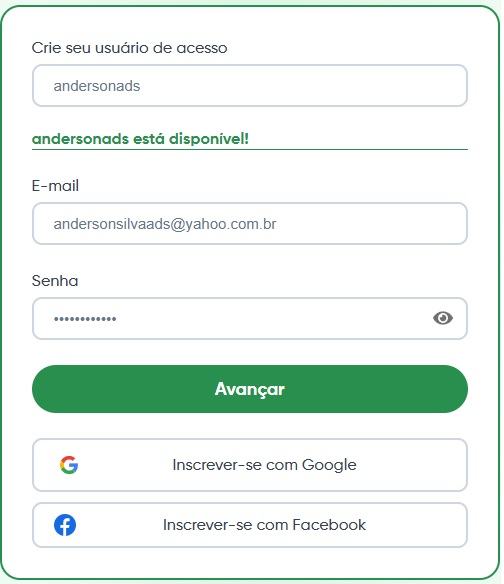
\includegraphics{images/np1/001-bling-cadastro.jpg} 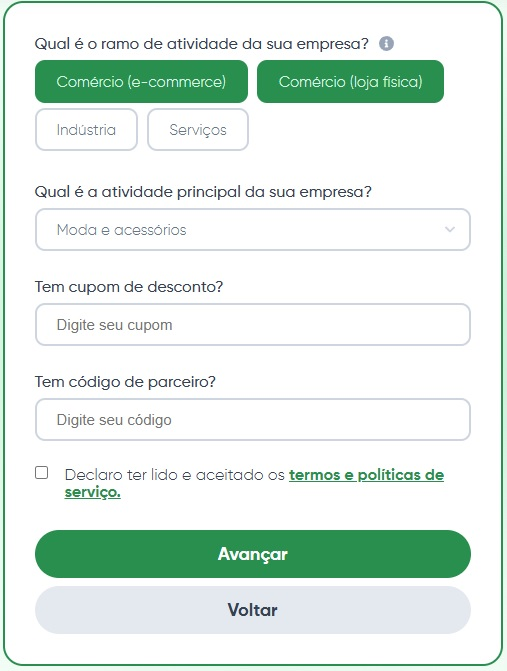
\includegraphics{images/np1/002-bling-selecionar-area-comercial.jpg} 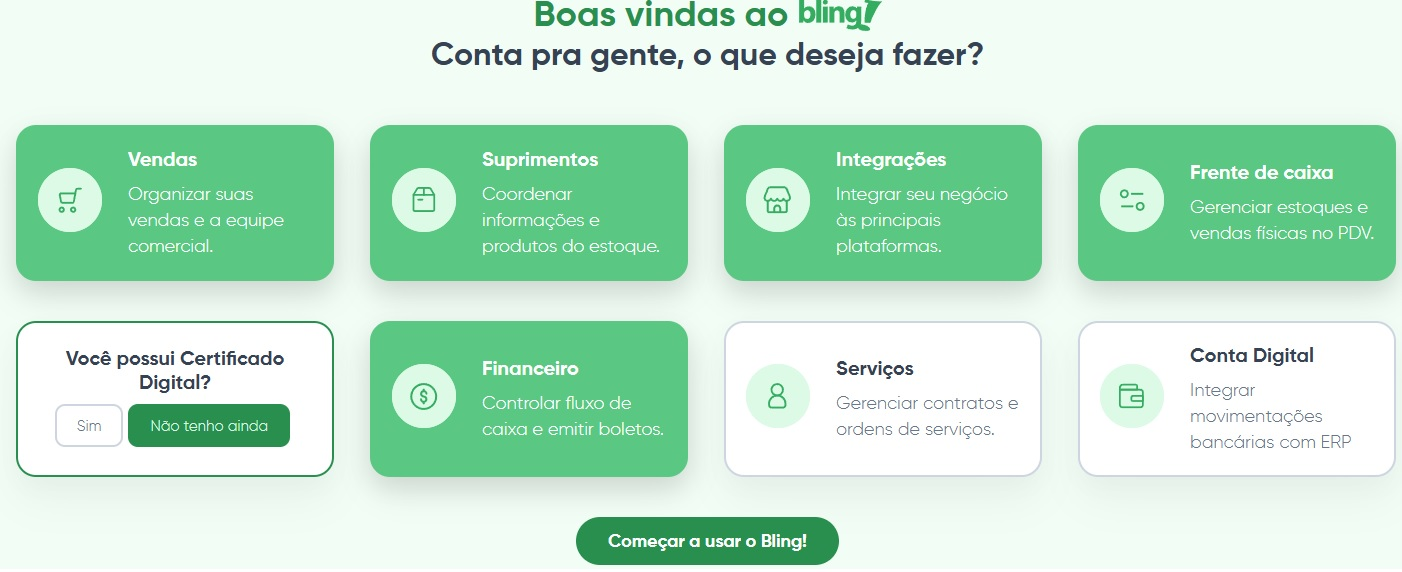
\includegraphics{images/np1/003-bling-escolher-modulos-erp.jpg} 
\includegraphics{images/np1/004-bling-conta-criada.jpg} 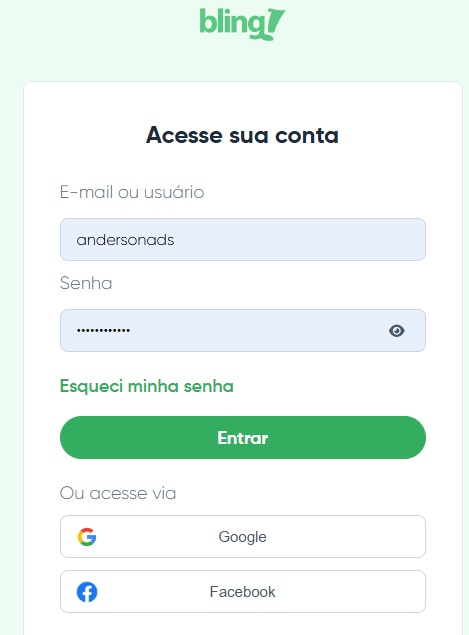
\includegraphics{images/np1/005-bling-logar-usuario-senha.jpg}

\subsubsection{Começar a cadastrar EMPRESA (Conceito de ``Módulo CONTROLE CADASTROS'' dos ERPs)}\label{comeuxe7ar-a-cadastrar-empresa-conceito-de-muxf3dulo-controle-cadastros-dos-erps}

\paragraph{Começar a cadastrar a EMPRESA (pessoa física ou jurídica)}\label{comeuxe7ar-a-cadastrar-a-empresa-pessoa-fuxedsica-ou-juruxeddica}

\includegraphics{images/np1/006-bling-identificar-pessoa-endereço.jpg} 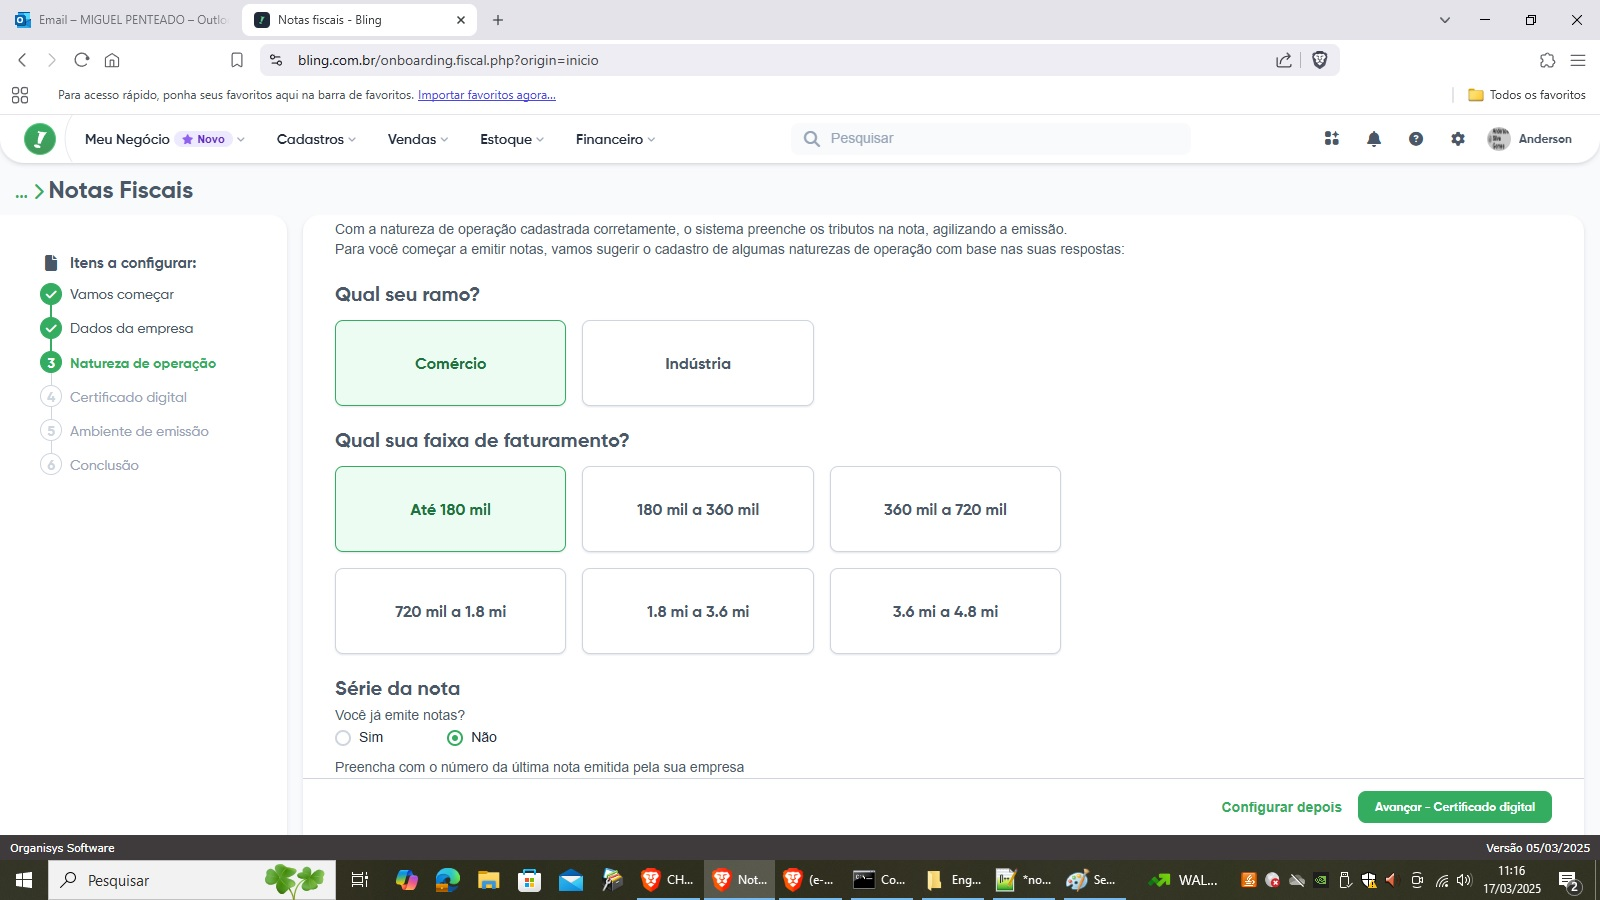
\includegraphics{images/np1/007-bling-natureza-negocio.jpg} 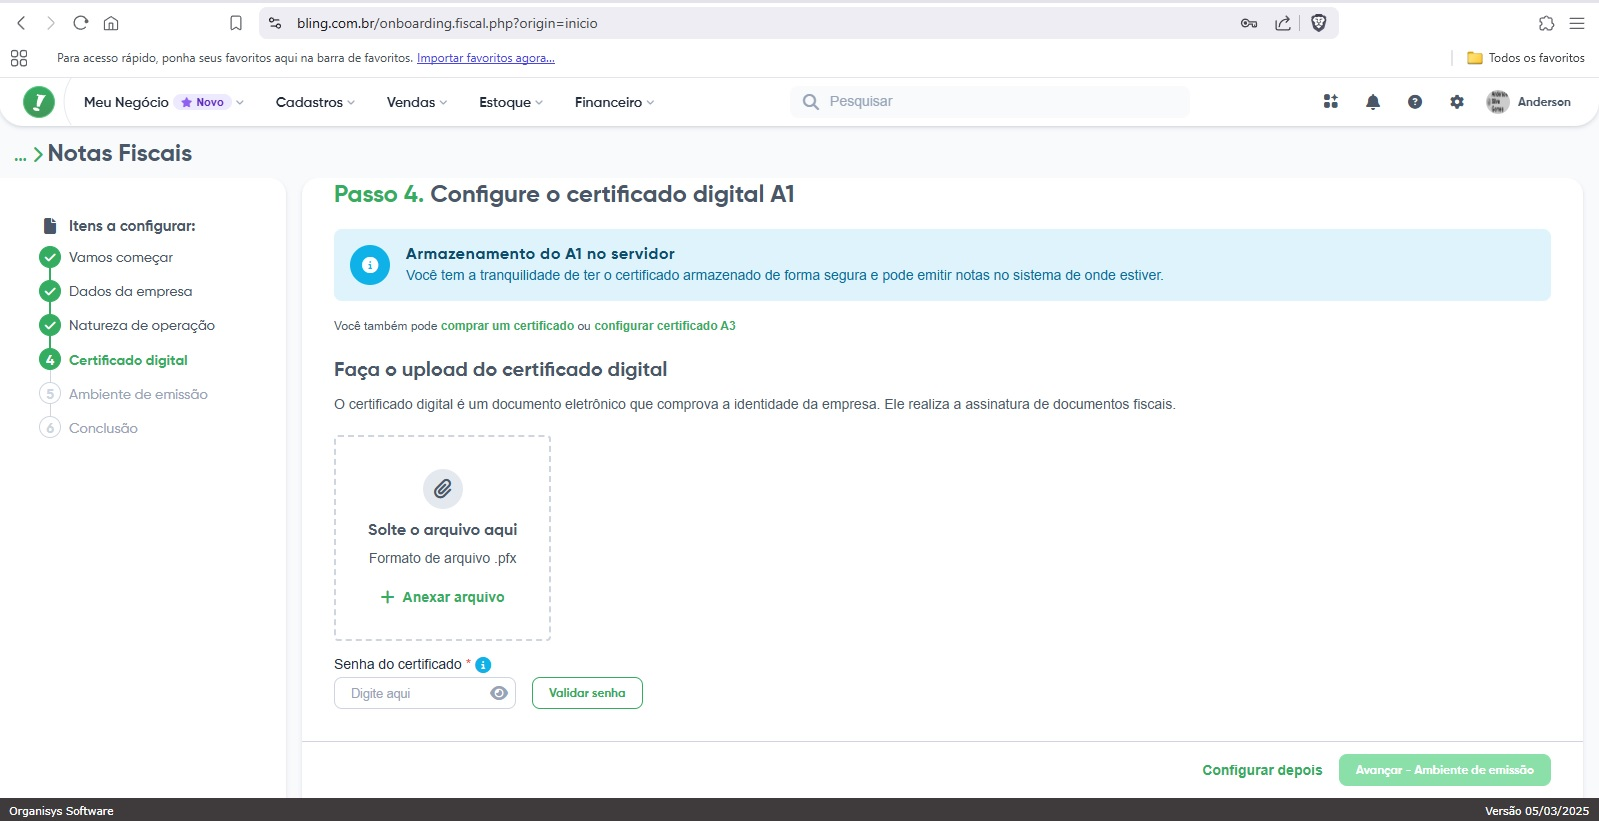
\includegraphics{images/np1/008-bling-certificado-digital-fisco-nota-fiscal.jpg}

\paragraph{Começar a cadastrar as categorias dos produtos (pessoa física ou jurídica)}\label{comeuxe7ar-a-cadastrar-as-categorias-dos-produtos-pessoa-fuxedsica-ou-juruxeddica}

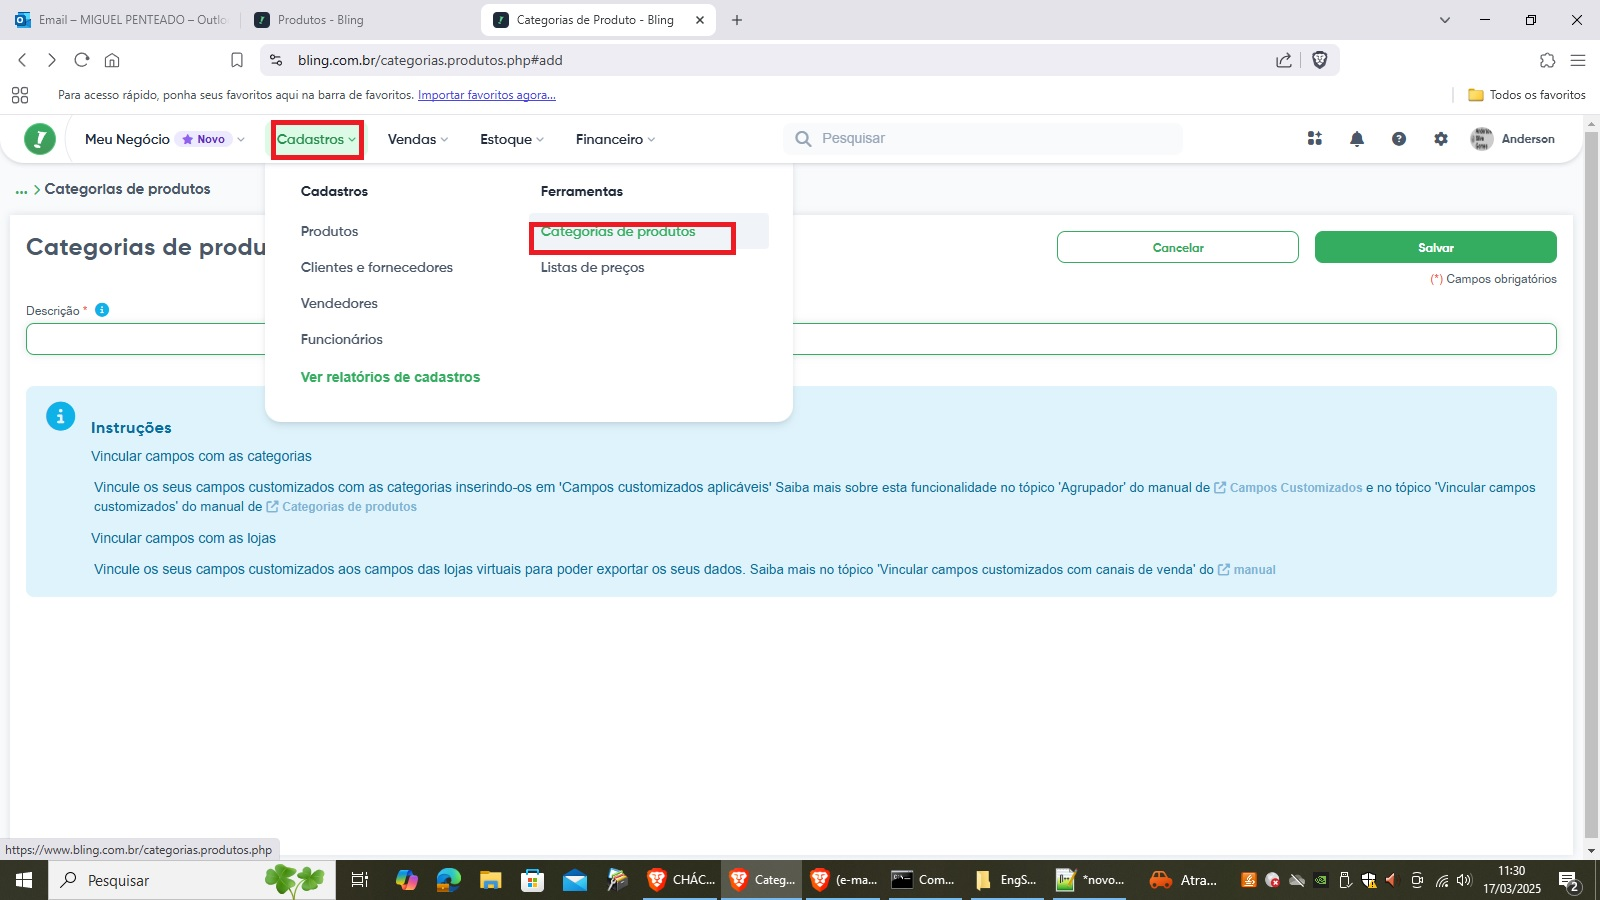
\includegraphics{images/np1/009-bling-cadastrar-categorias-produtos.jpg} 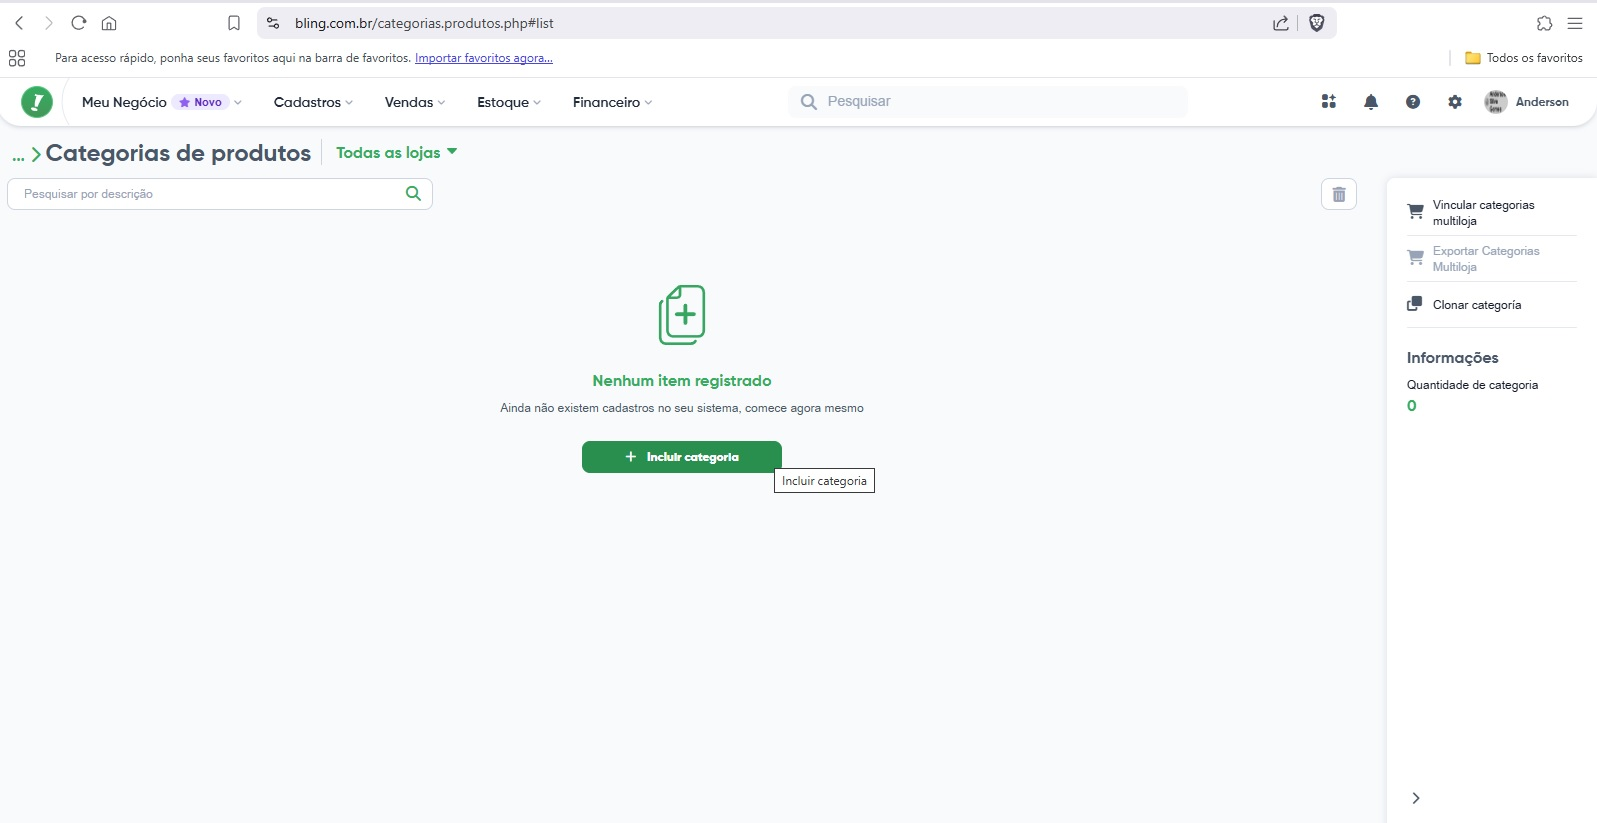
\includegraphics{images/np1/010-bling-cadastrar-categorias-produtos-tela-lista-categorias.jpg} 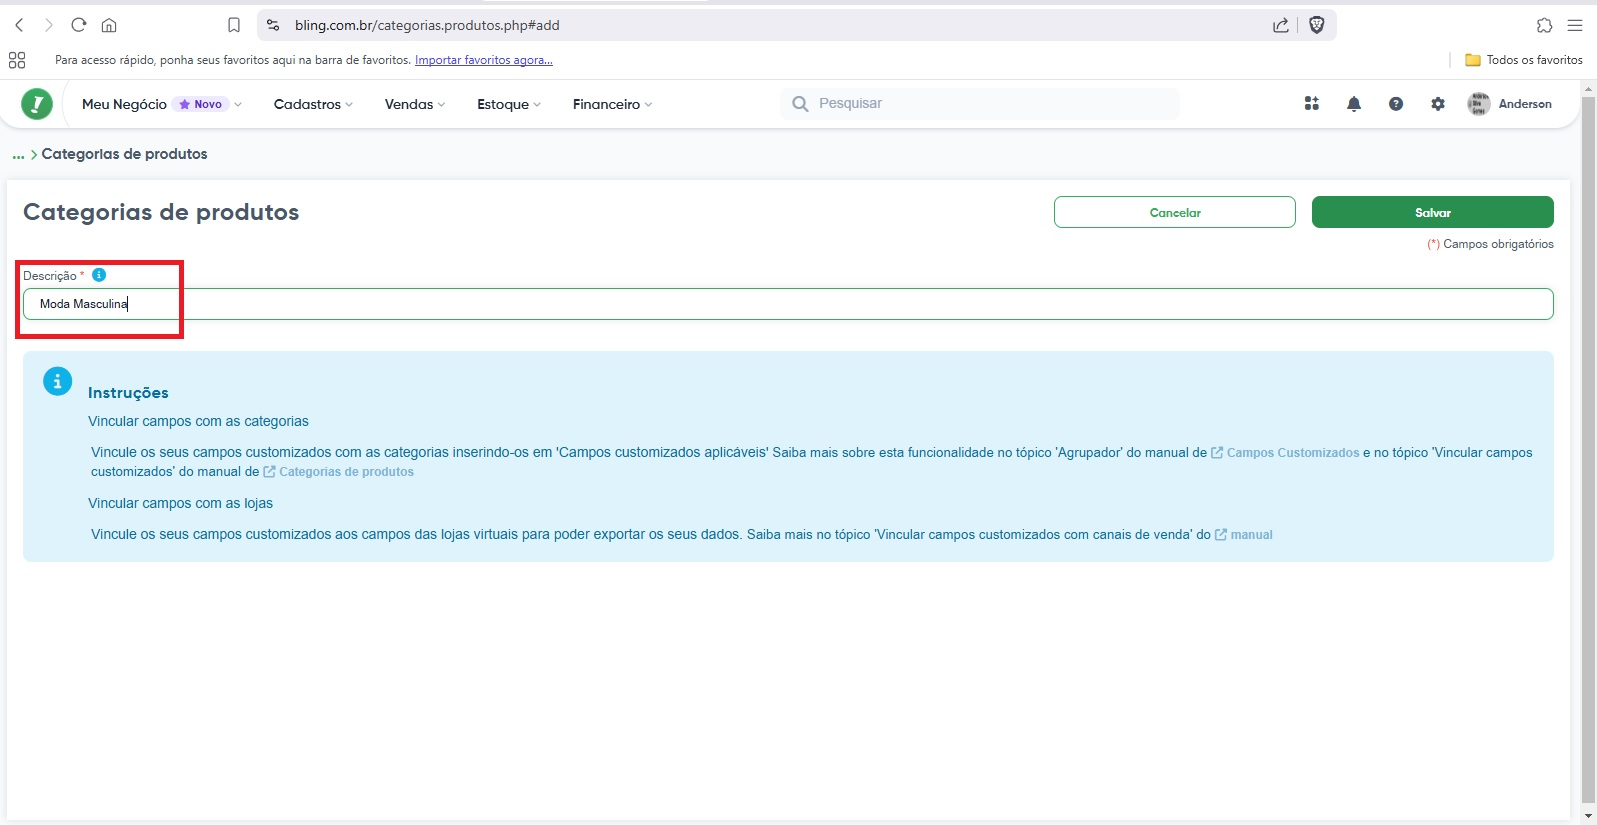
\includegraphics{images/np1/011-bling-cadastrar-moda-masculina.jpg} 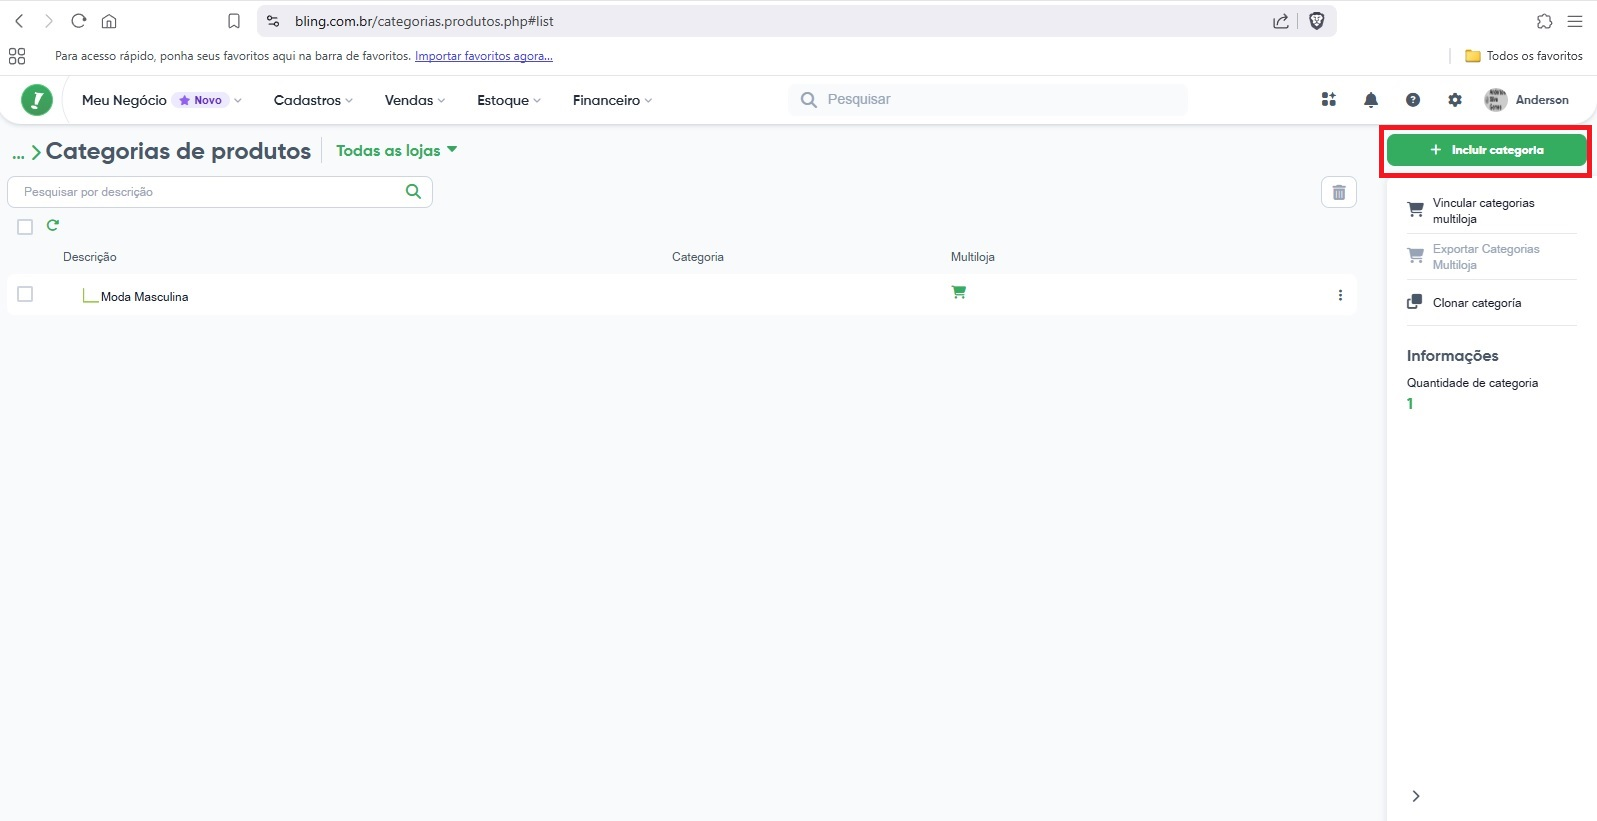
\includegraphics{images/np1/012-bling-cadastrar-categorias-produtos-tela-lista-categorias-inserir-moda-feminina.jpg} 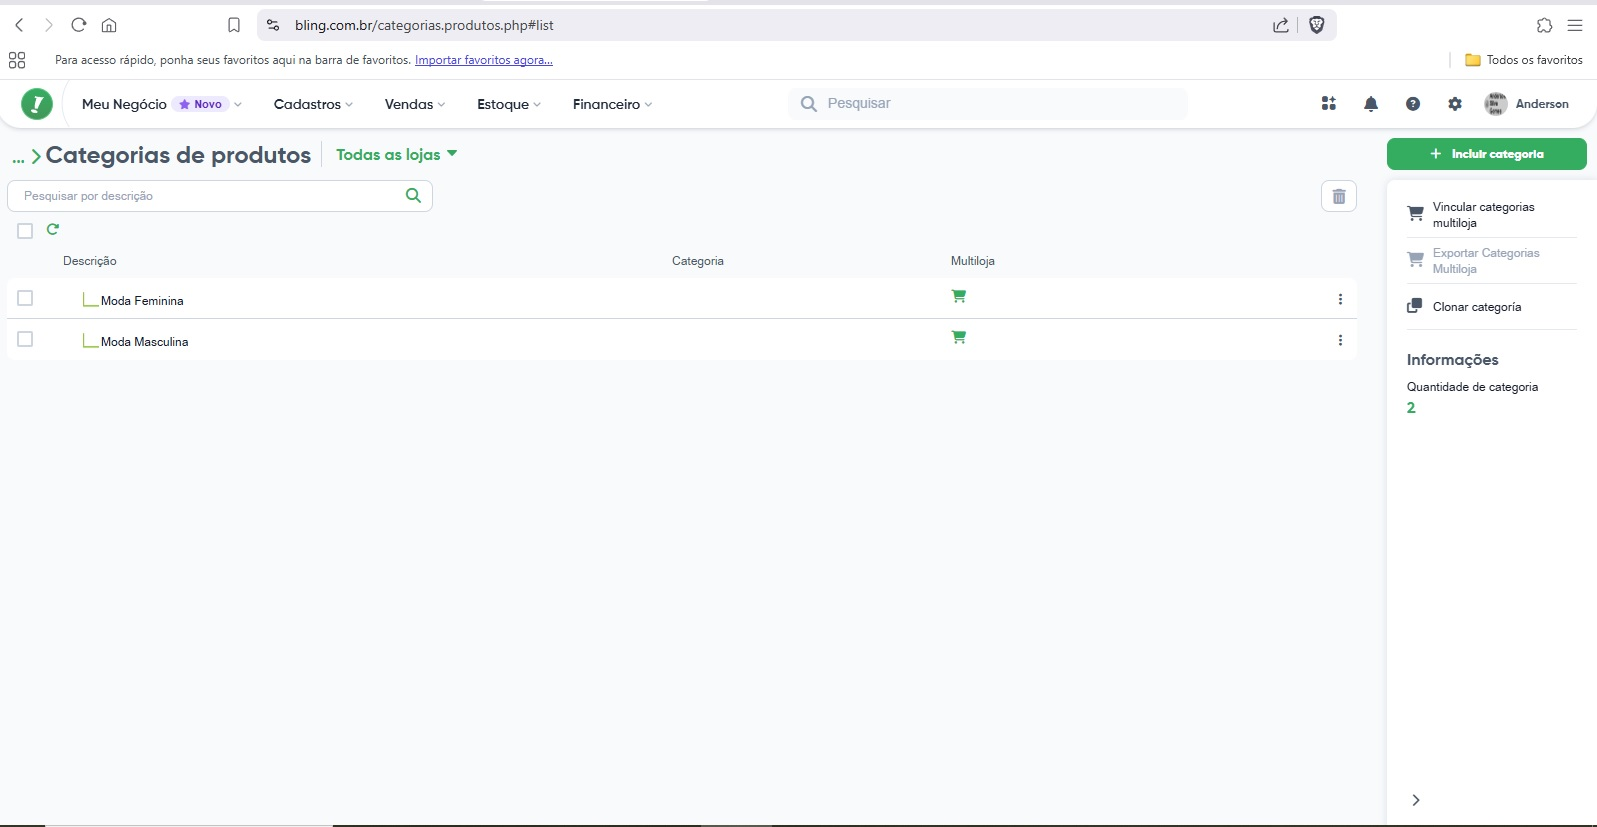
\includegraphics{images/np1/014-bling-cadastrar-subcategoria-moda-masculina-camiseta.jpg} 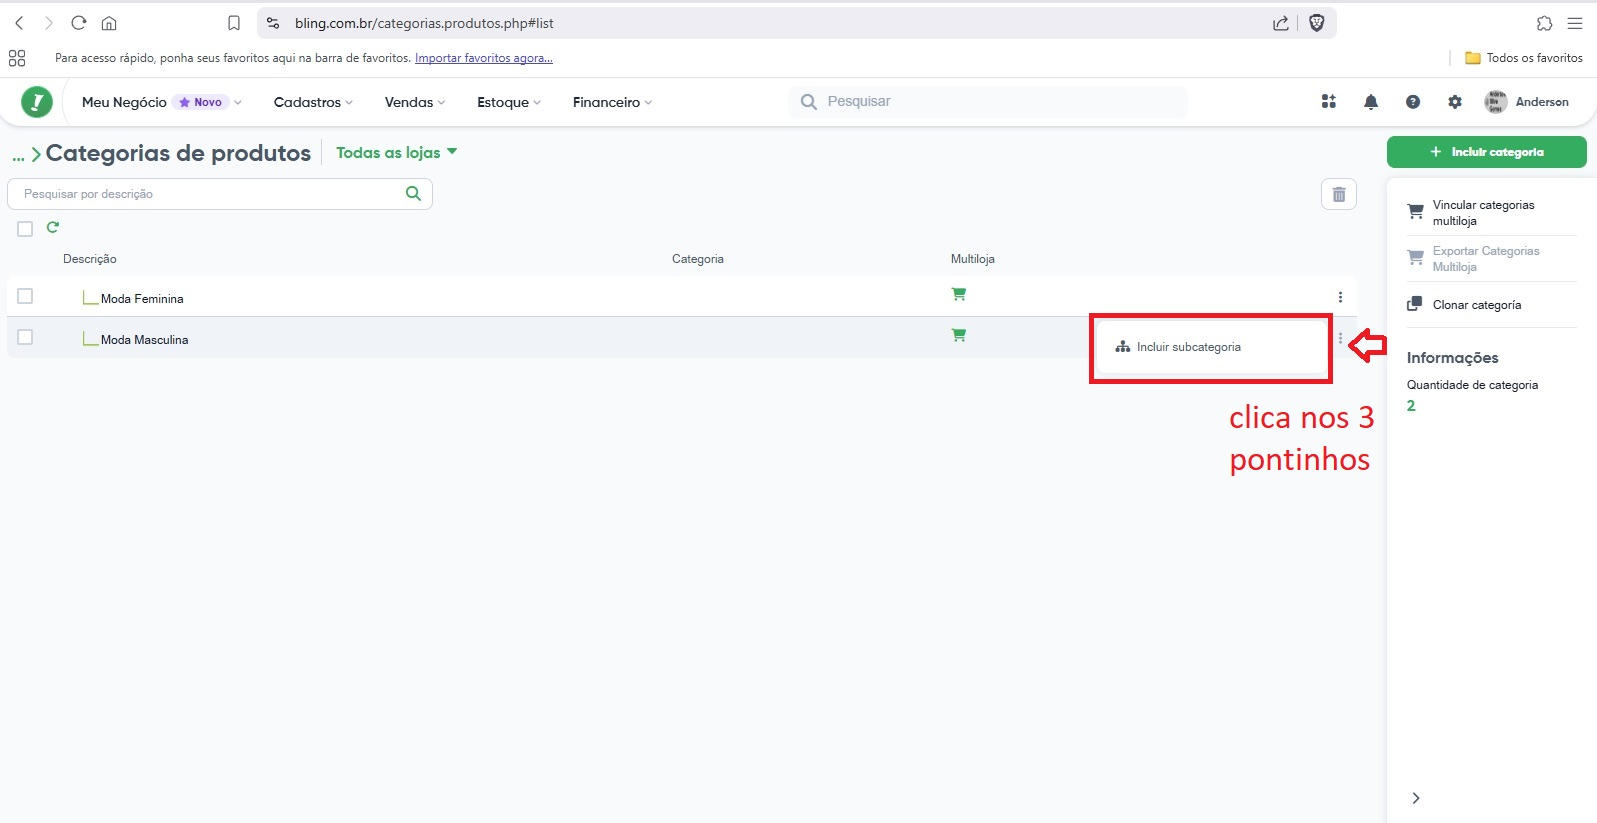
\includegraphics{images/np1/015-bling-cadastrar-subcategoria-moda-masculina-camiseta.jpg} 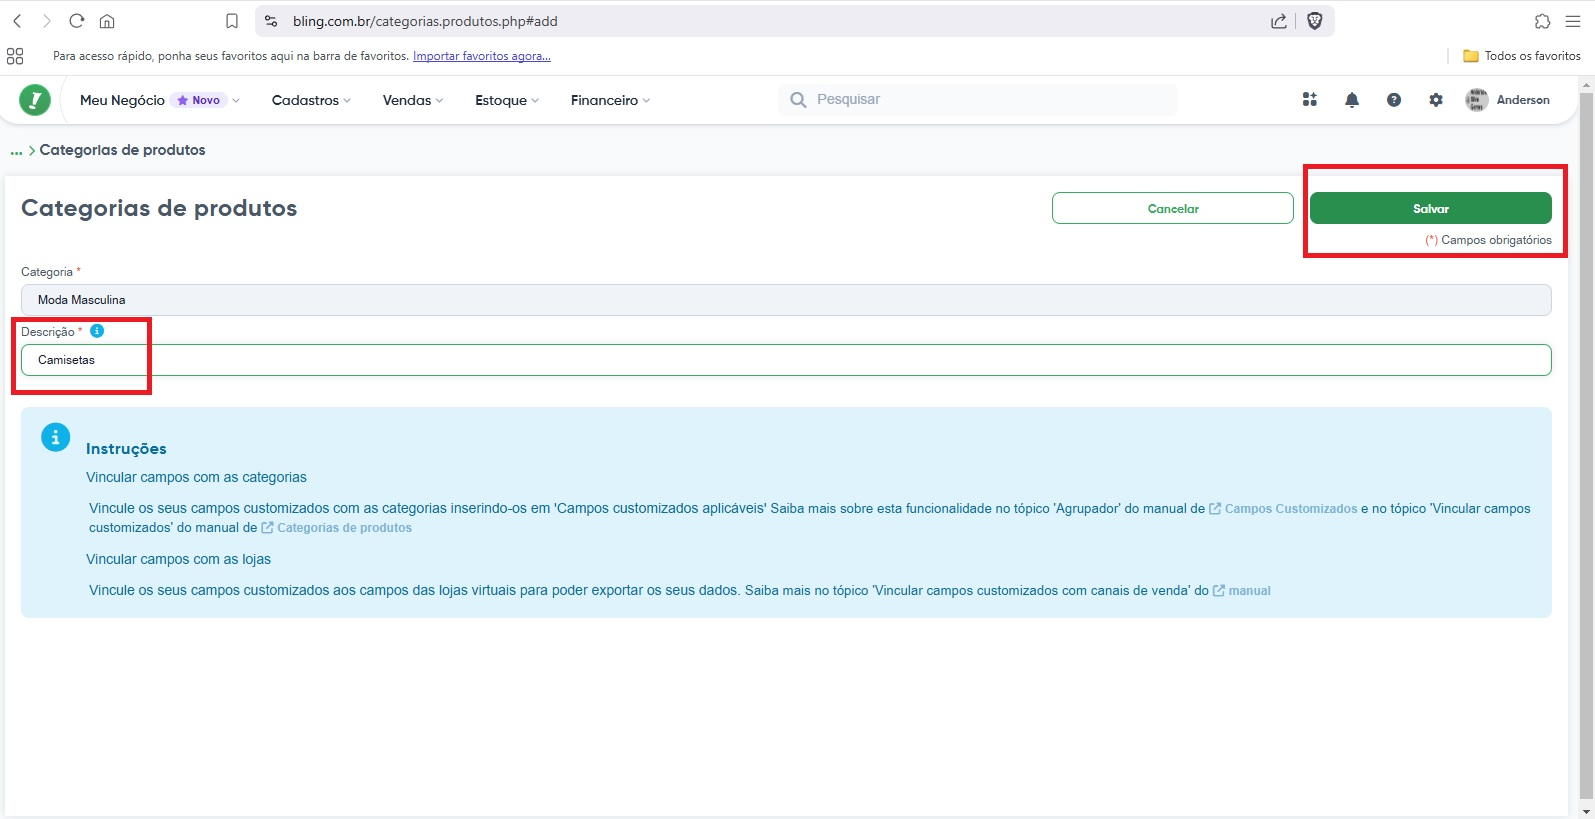
\includegraphics{images/np1/016-bling-confirmar-cadastro-camisetas-em-moda-masculina.jpg} 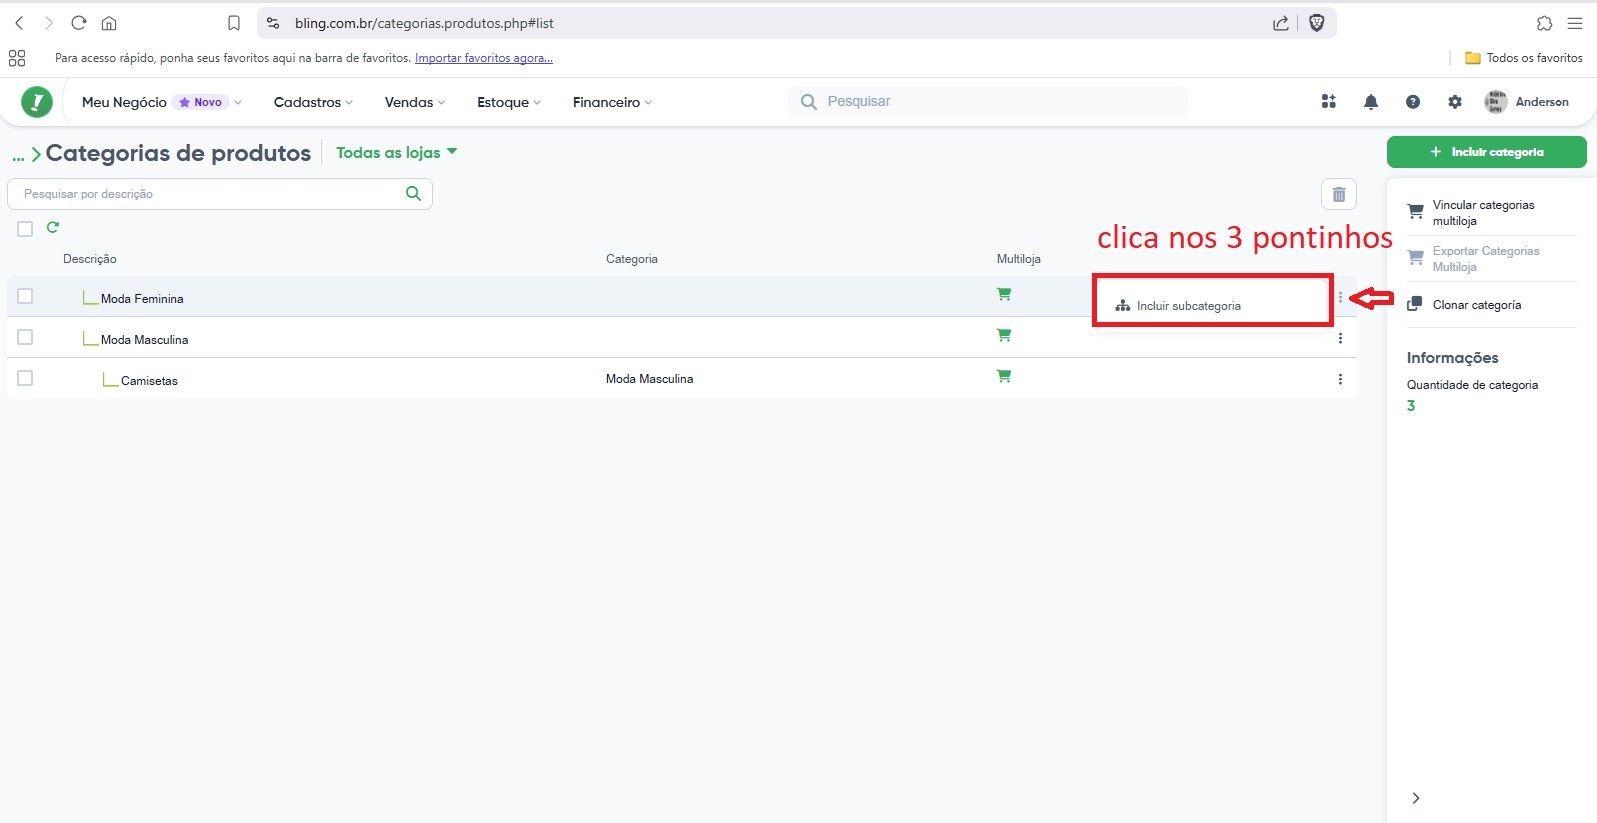
\includegraphics{images/np1/017-bling-cadastrar-subcategoria-moda-feminina-vestido.jpg} 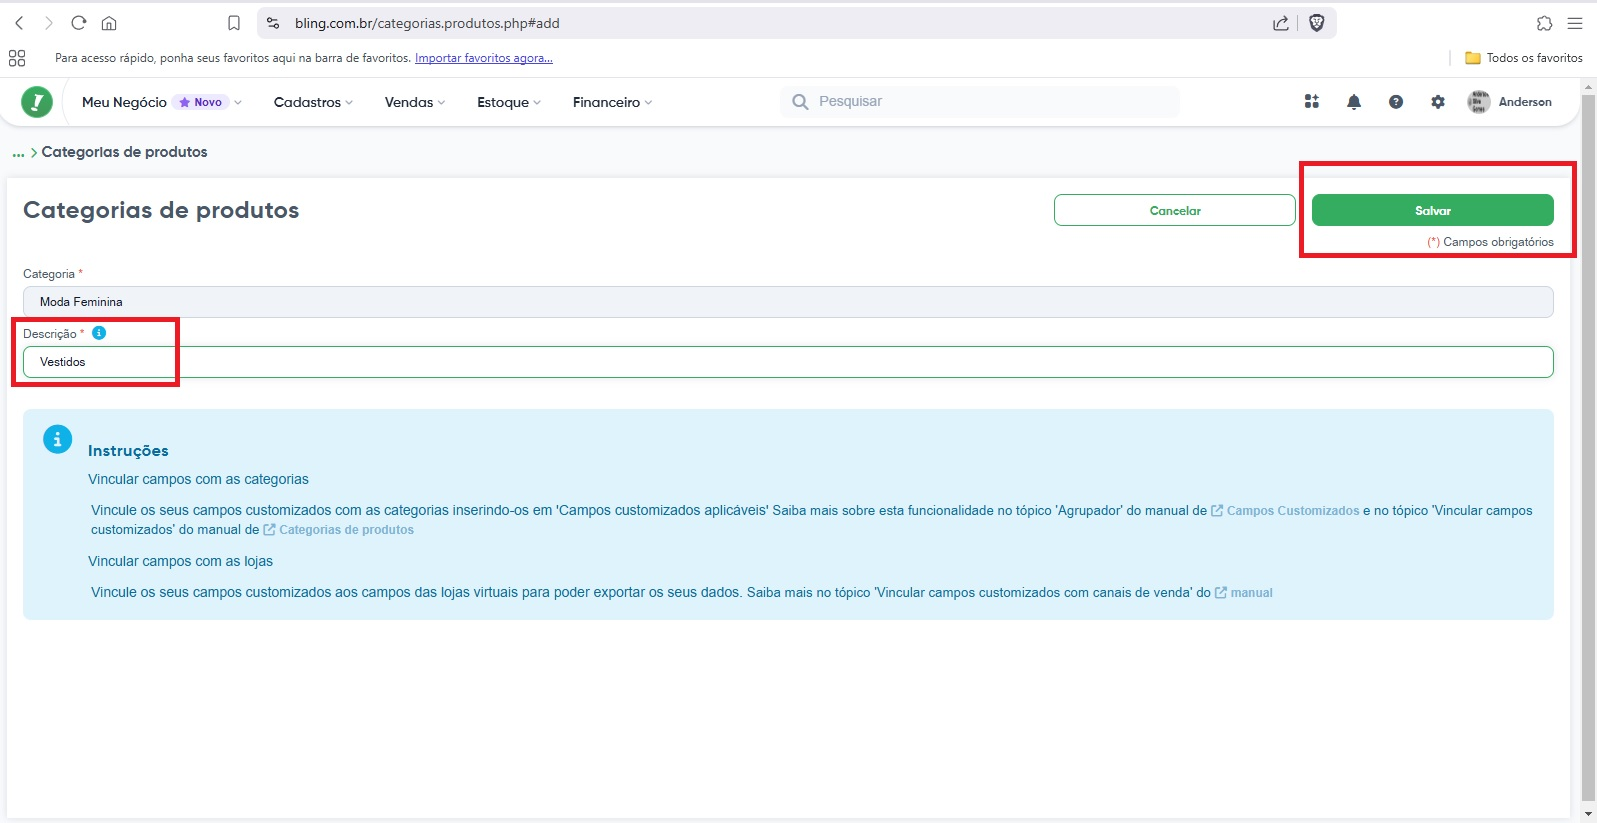
\includegraphics{images/np1/018-bling-confirmar-cadastro-vestidos-em-moda-feminina.jpg} 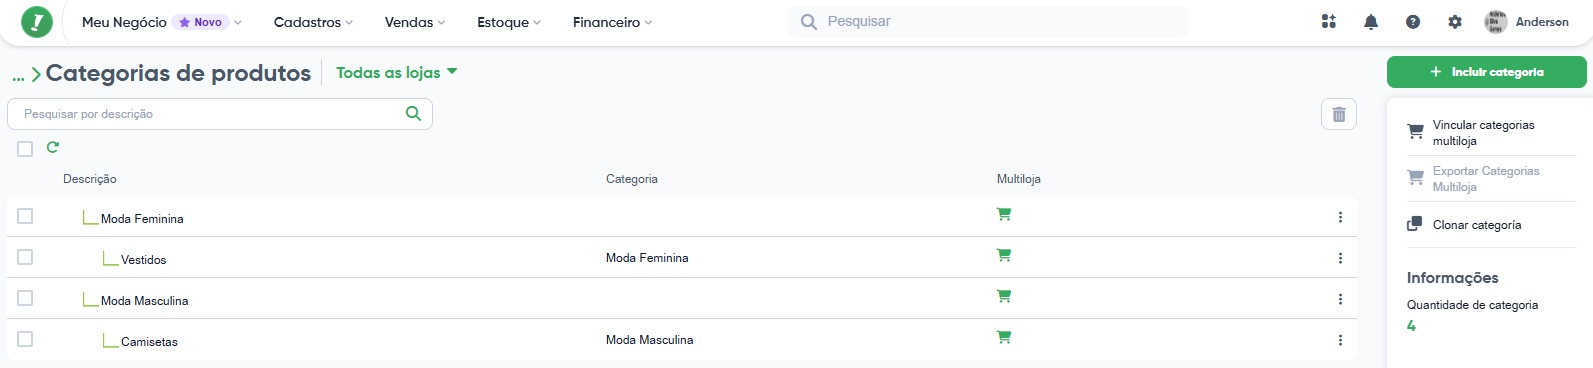
\includegraphics{images/np1/019-categorias-cadastradas.jpg}

\paragraph{Começar a cadastrar os produtos (pessoa física ou jurídica)}\label{comeuxe7ar-a-cadastrar-os-produtos-pessoa-fuxedsica-ou-juruxeddica}

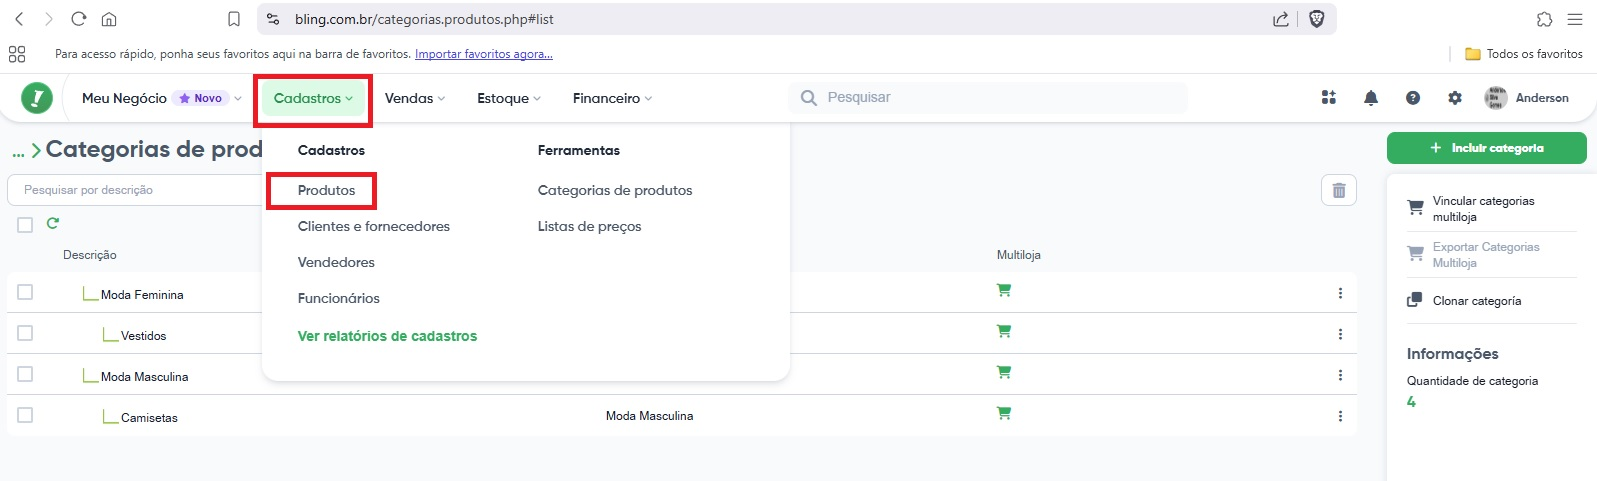
\includegraphics{images/np1/020-cadastrar-produtos.jpg} 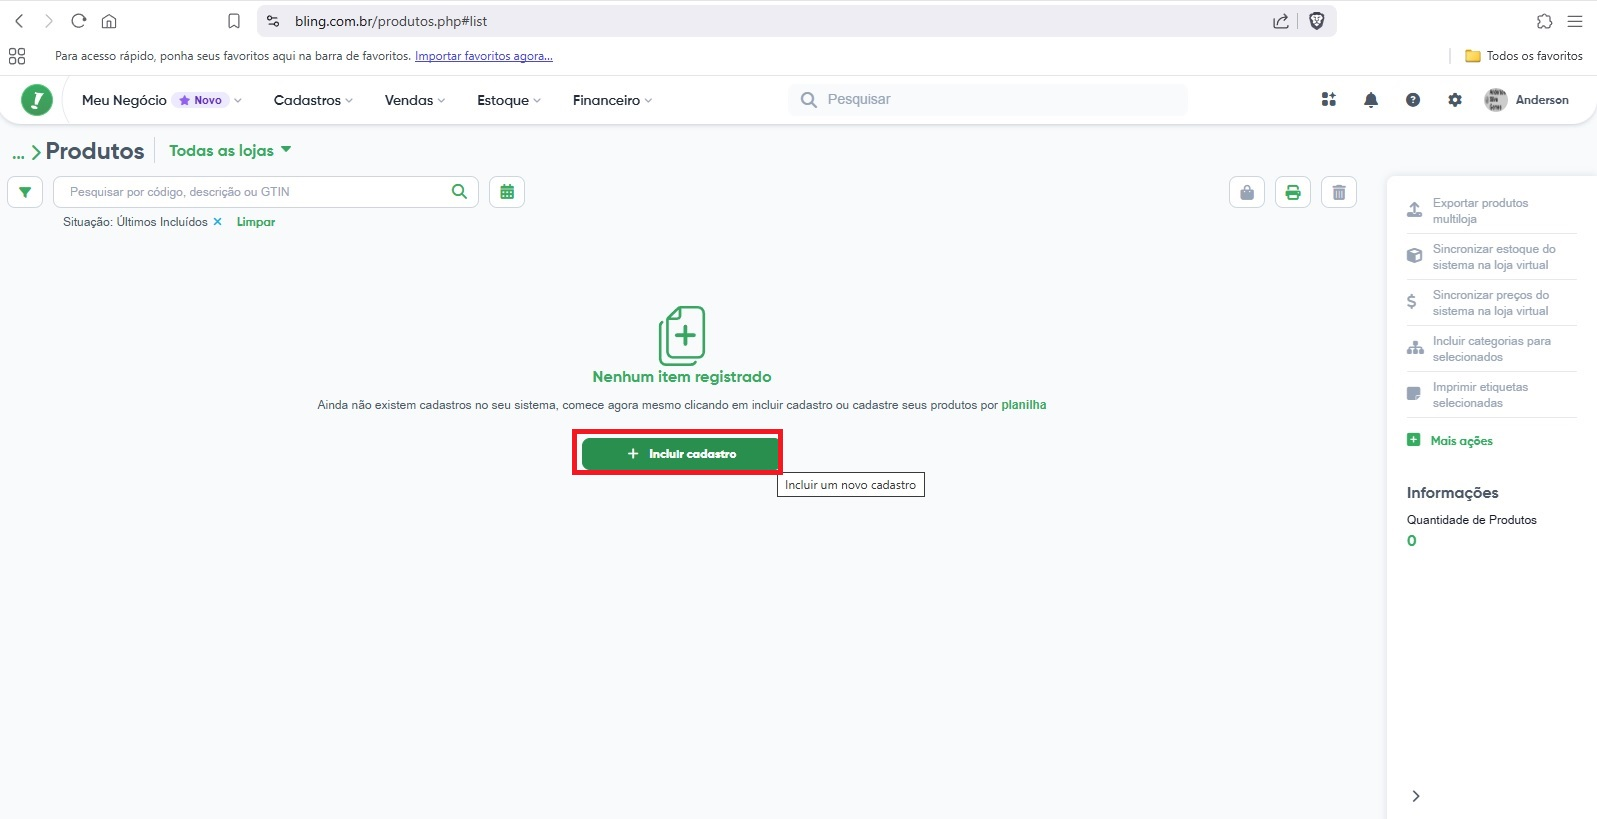
\includegraphics{images/np1/021-cadastro-produtos-inserir-produto.jpg} 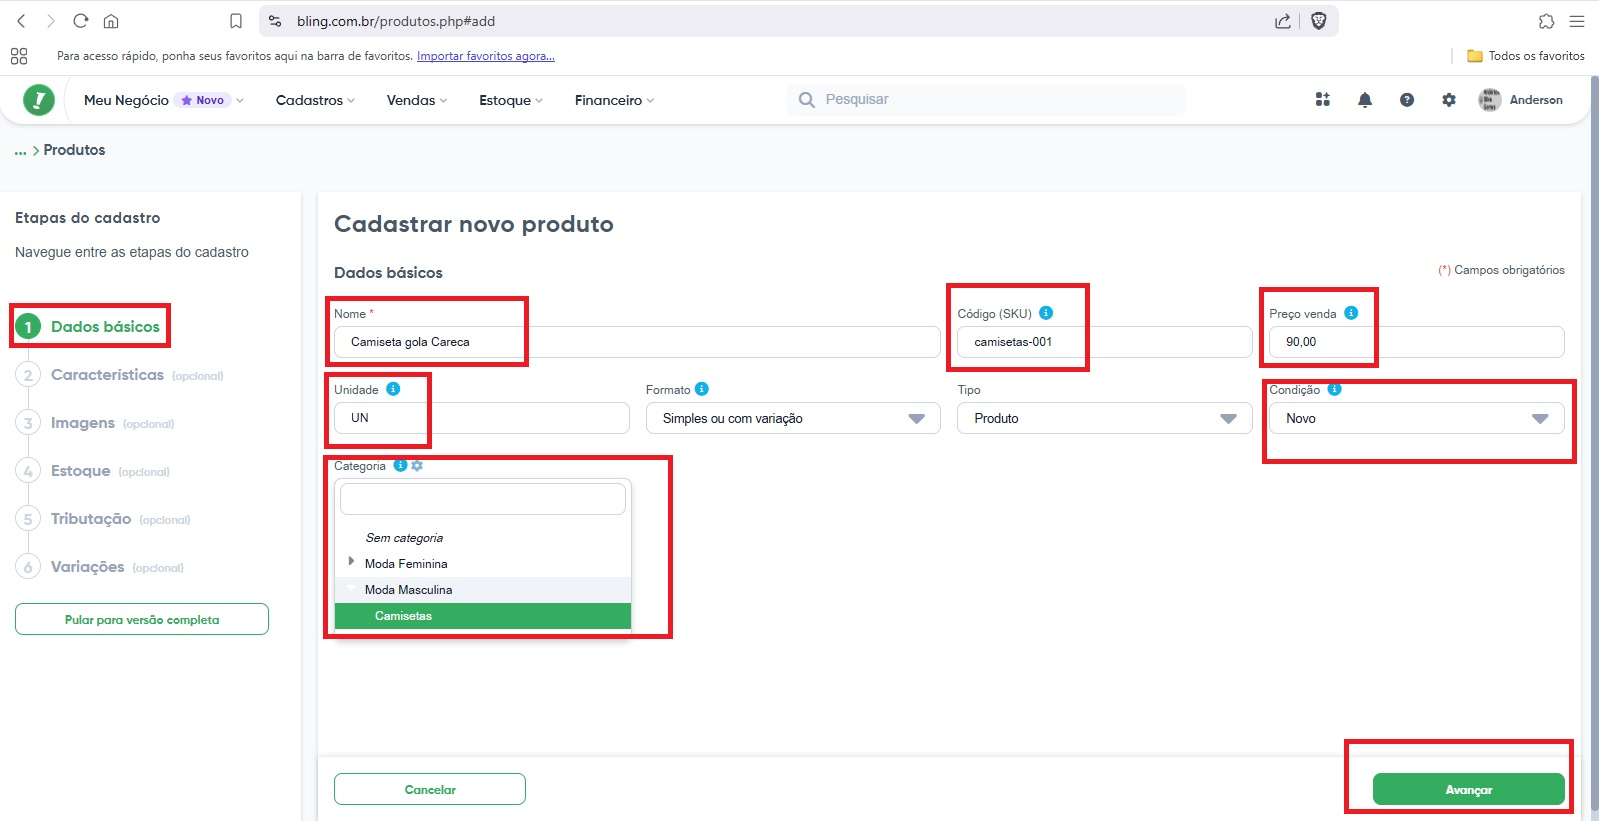
\includegraphics{images/np1/022-cadastro-produtos-inserir-produto-dados-basicos.jpg} 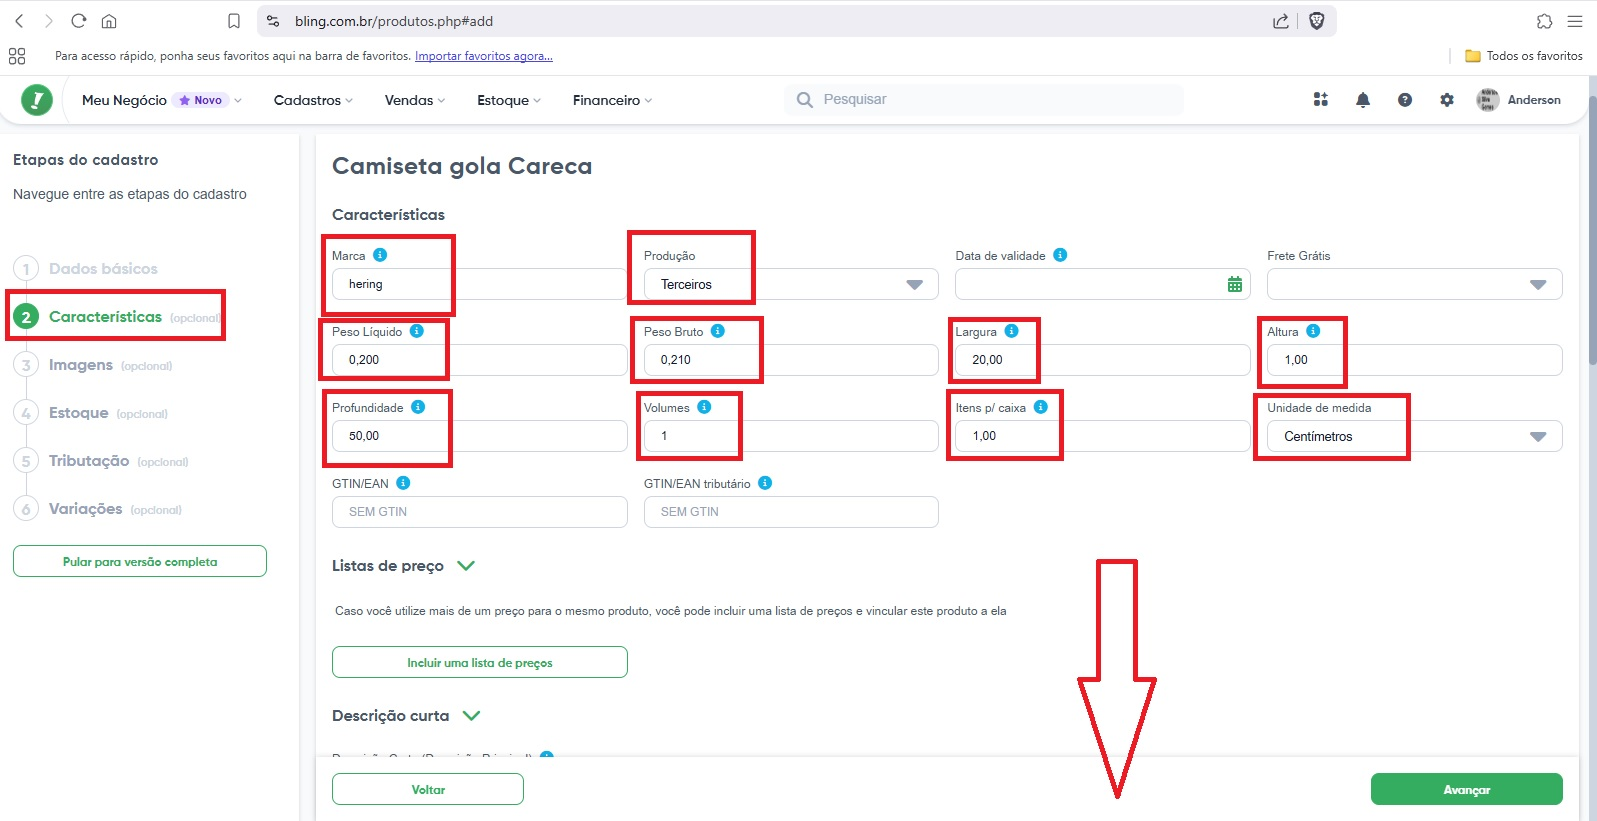
\includegraphics{images/np1/023-cadastro-produtos-inserir-detalhes-e-commerce.jpg} 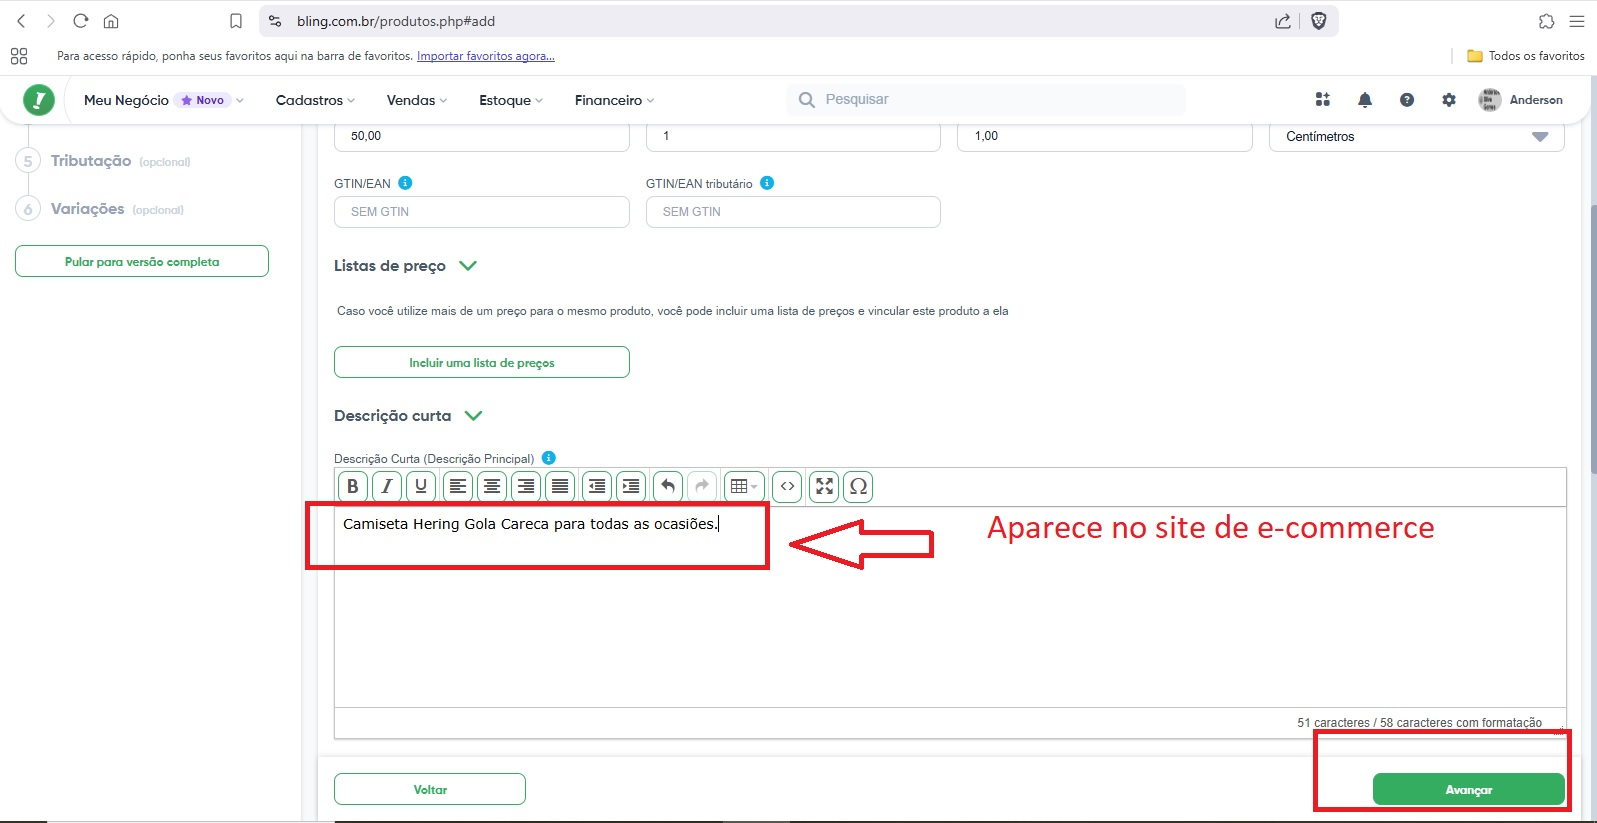
\includegraphics{images/np1/024-cadastro-produtos-inserir-detalhes-e-commerce-descricao.jpg} 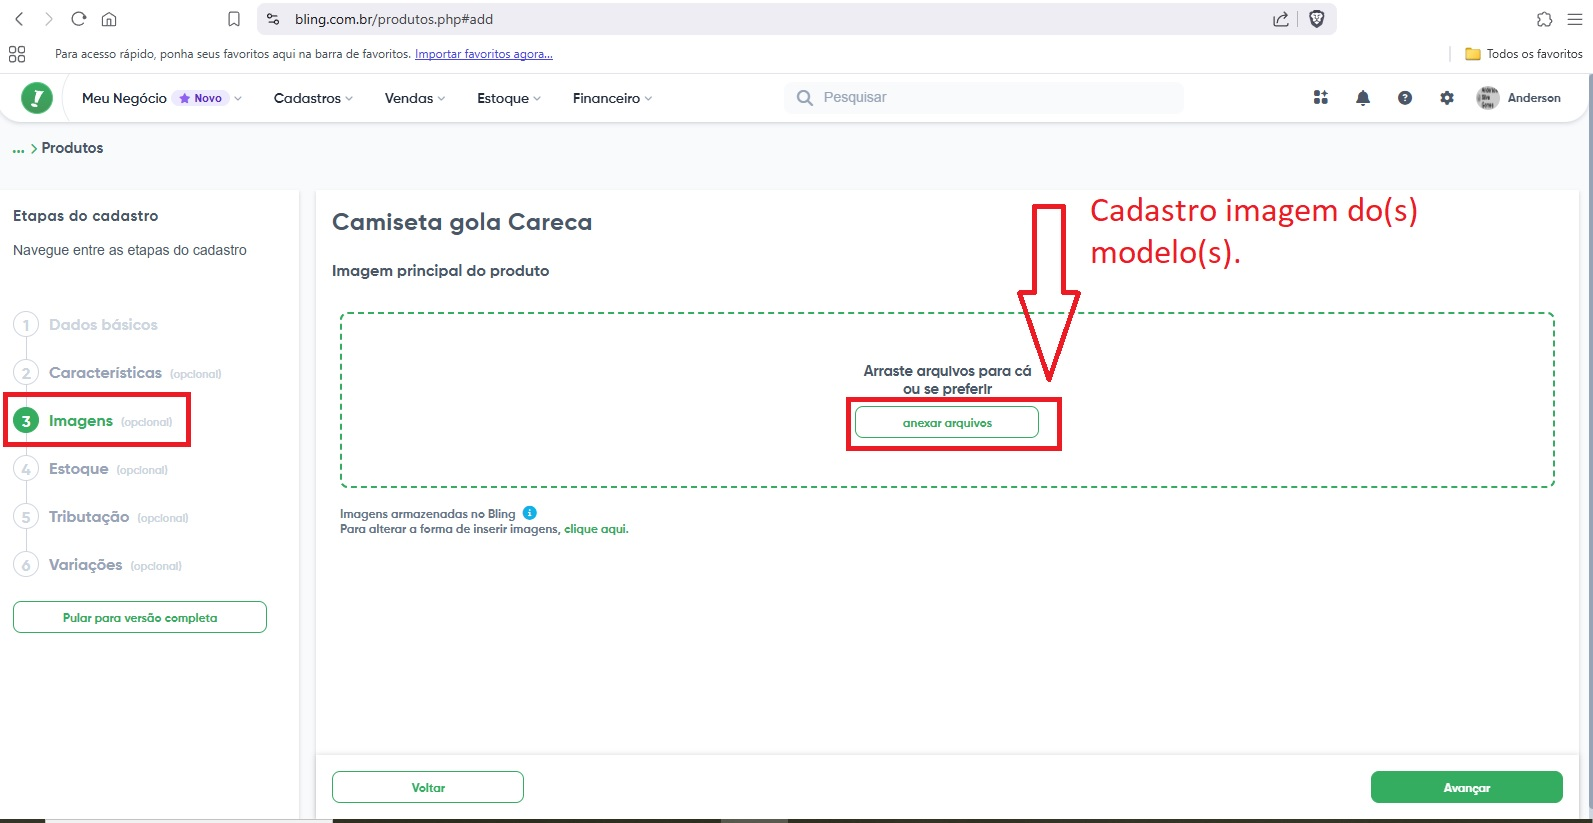
\includegraphics{images/np1/025-cadastro-produtos-inserir-imagem-produtos.jpg} 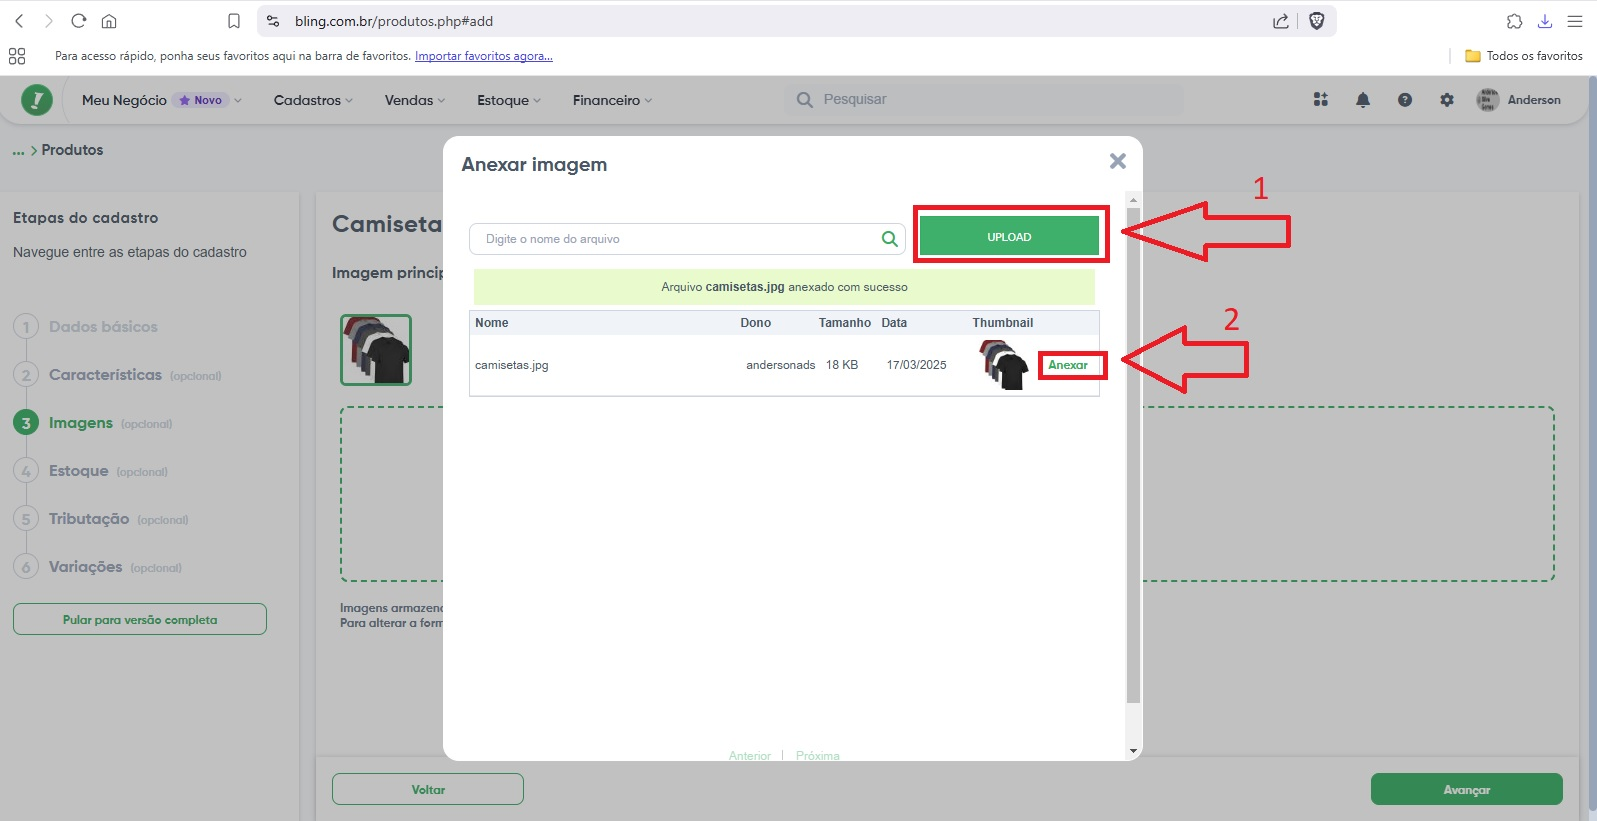
\includegraphics{images/np1/026-cadastro-produtos-inserir-imagem-produtos.jpg} 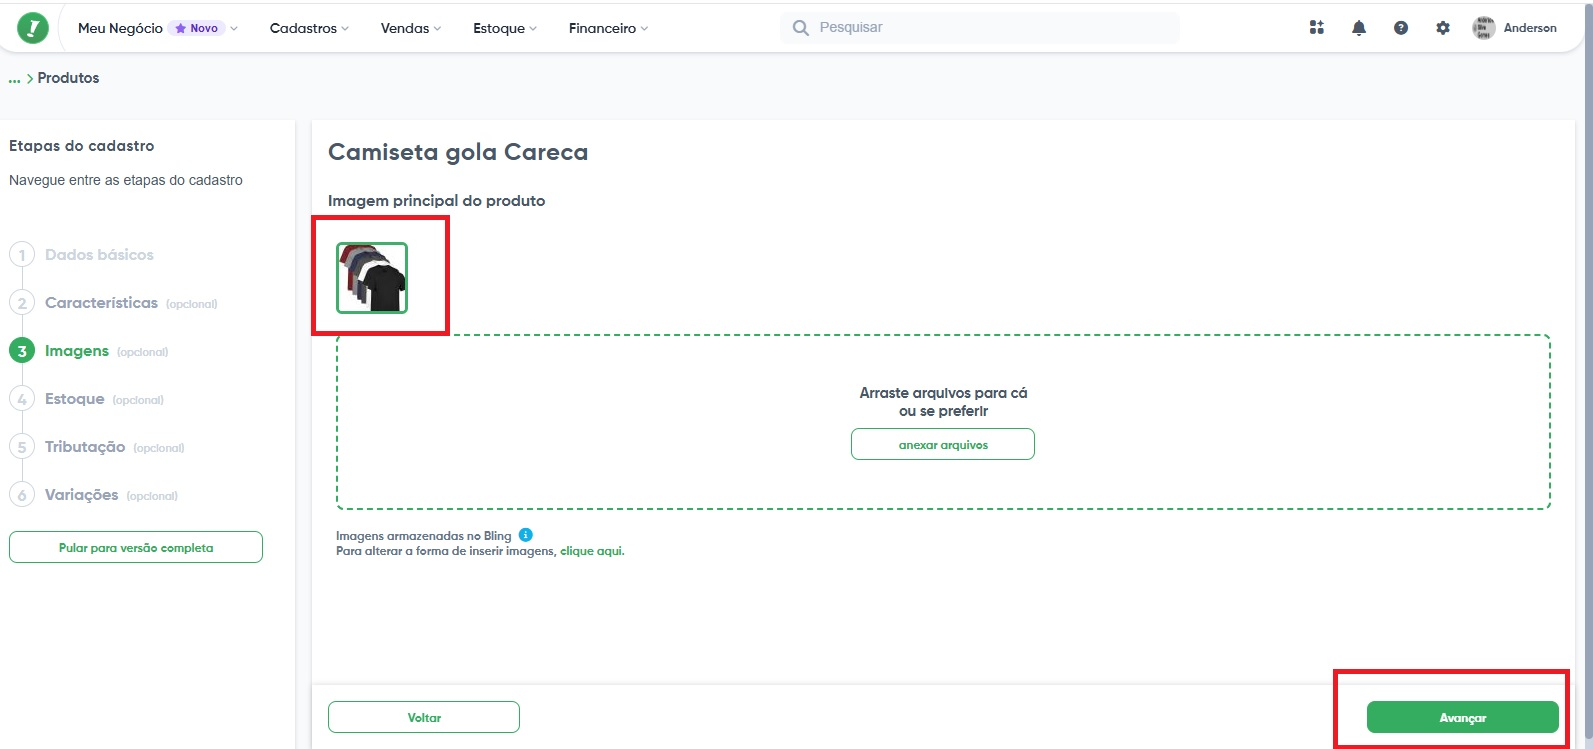
\includegraphics{images/np1/027-cadastro-produtos-inserir-imagem-produtos-cadastradas.jpg} 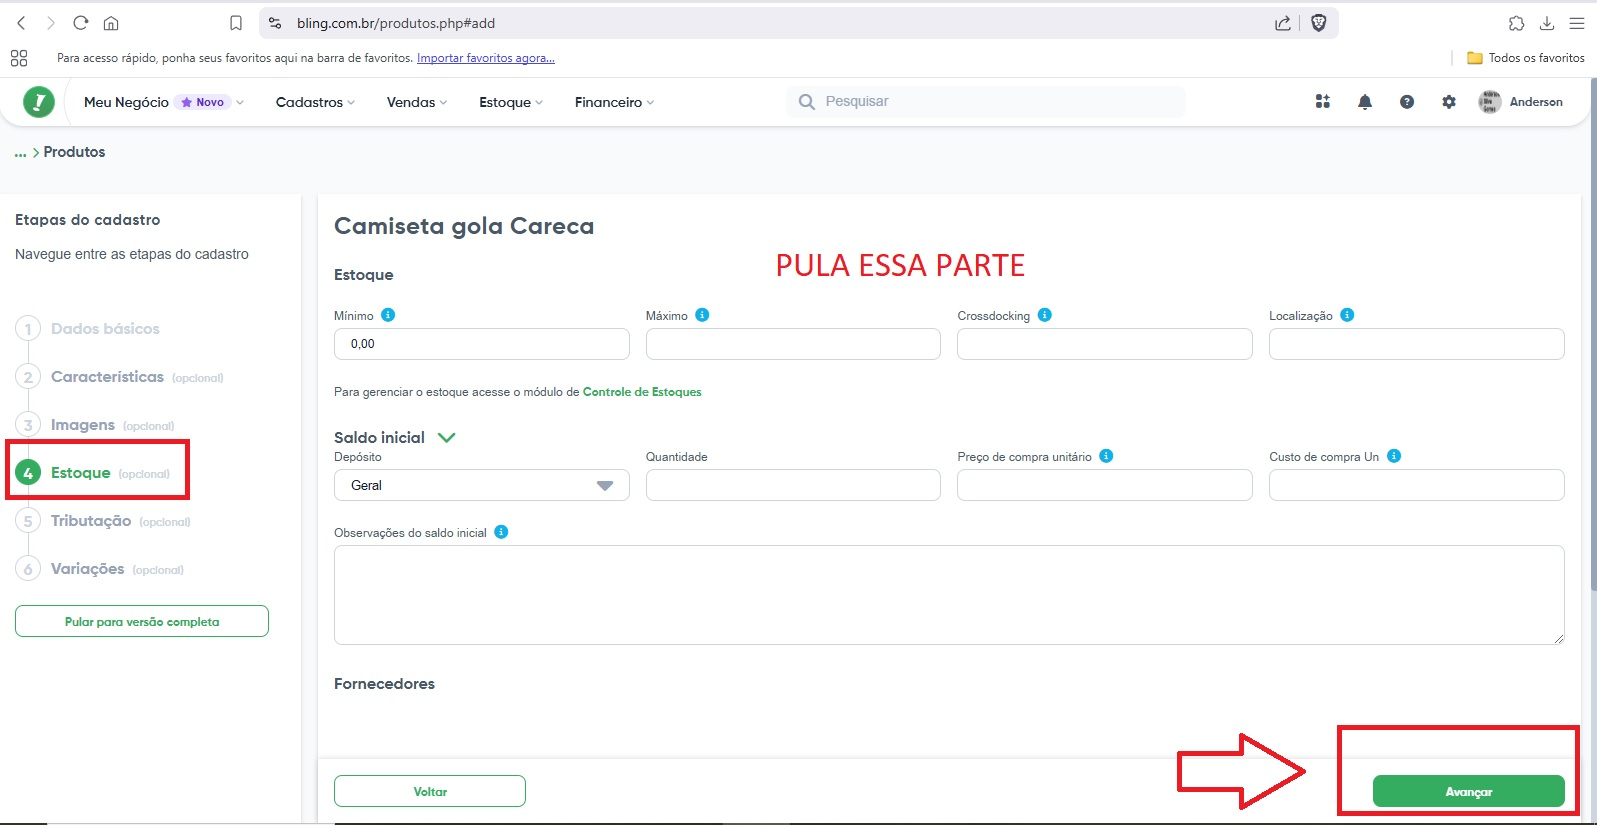
\includegraphics{images/np1/028-cadastro-produtos-quantidade-estoque.jpg} 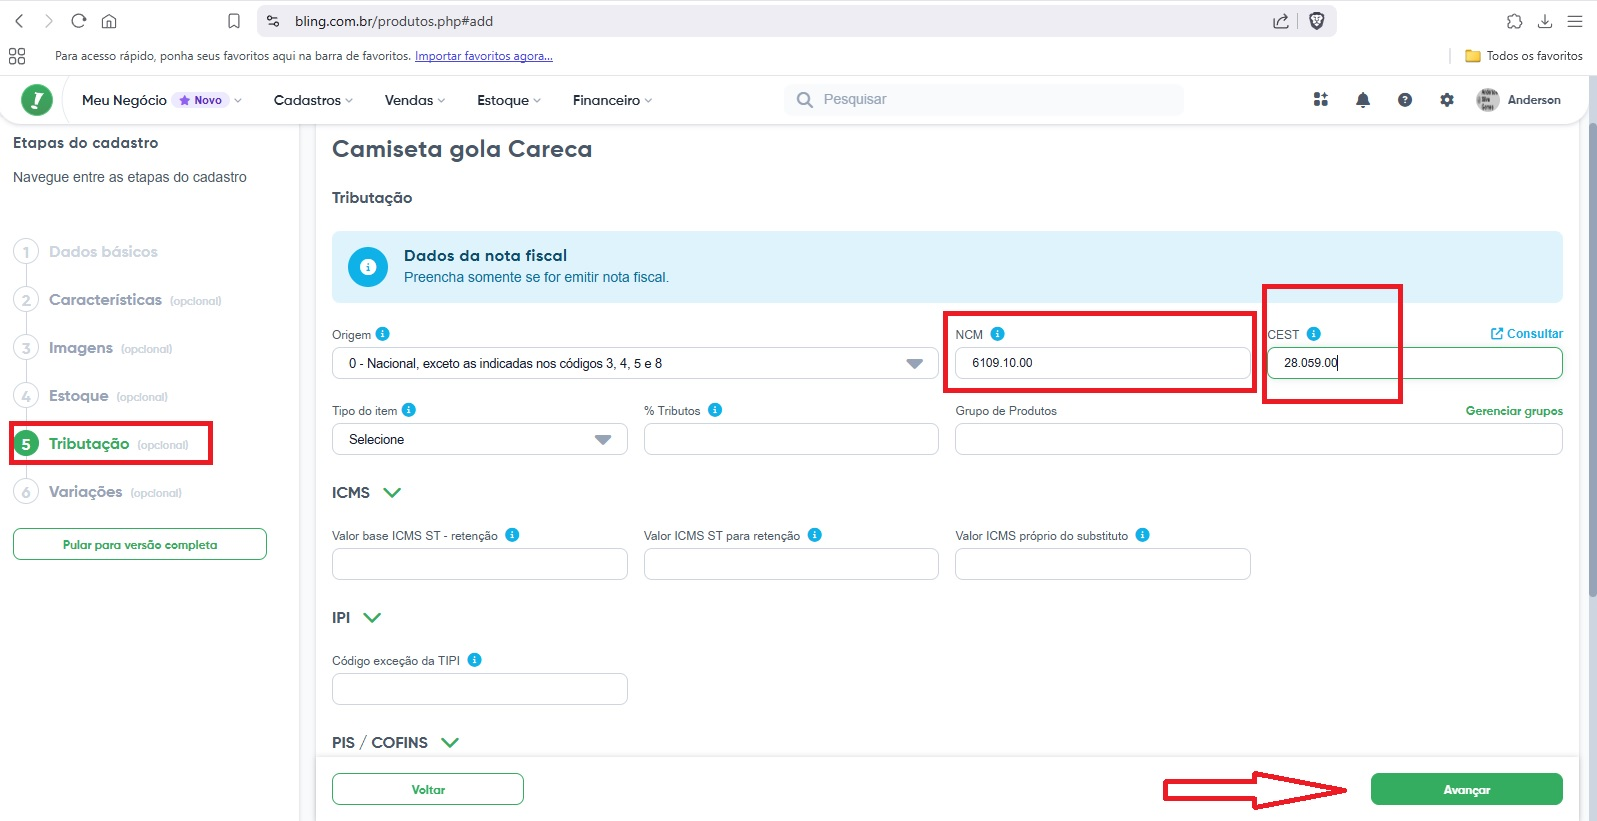
\includegraphics{images/np1/029-cadastro-produtos-fiscal-NCM-CEST.jpg} 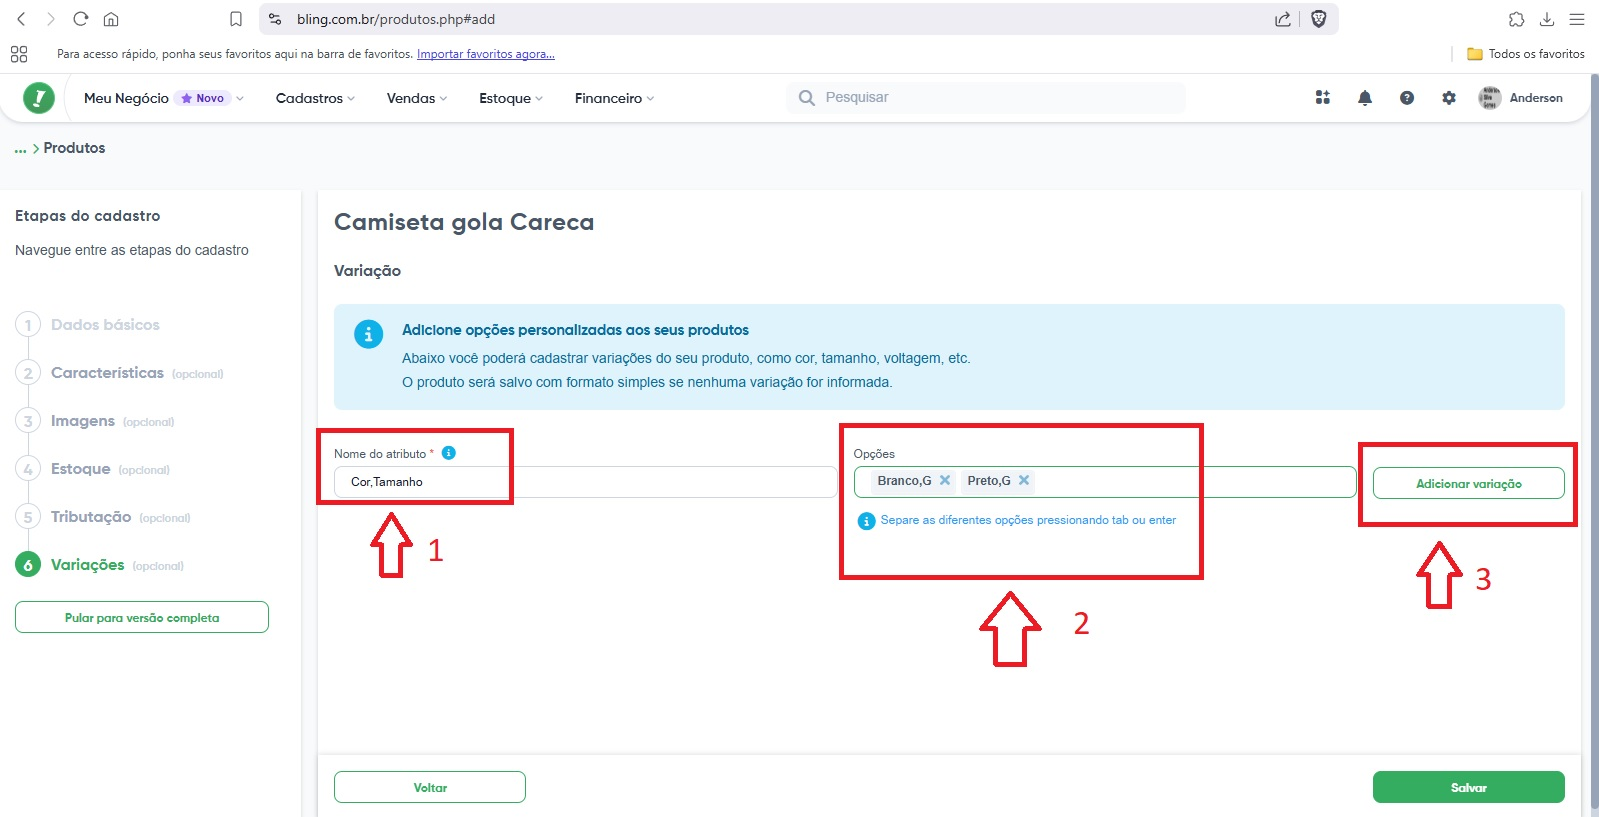
\includegraphics{images/np1/030-cadastro-produtos-variações-produto.jpg} 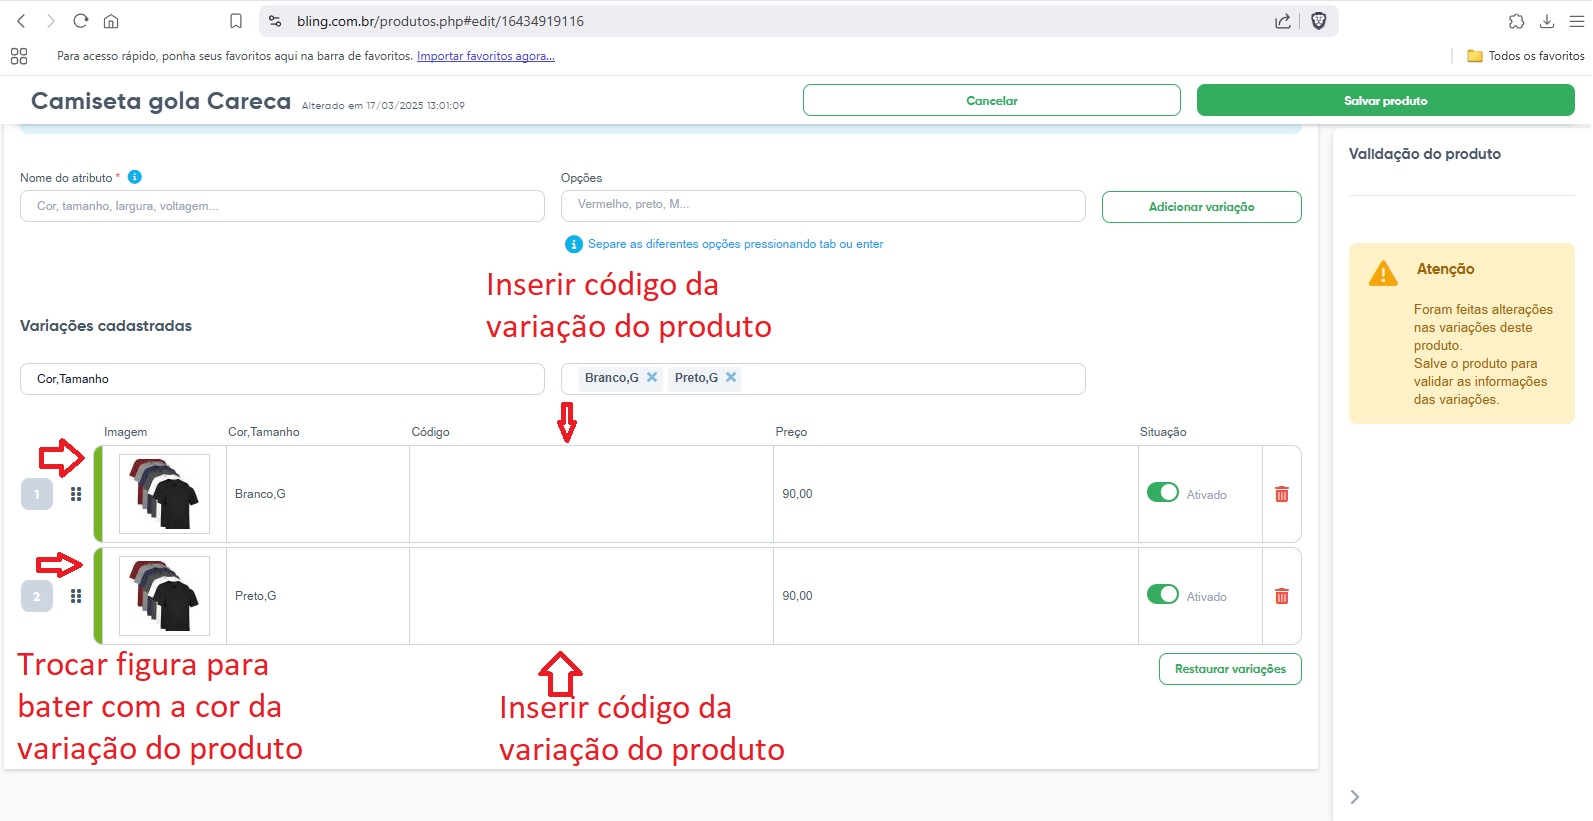
\includegraphics{images/np1/031-cadastro-produtos-variações-produto.jpg} 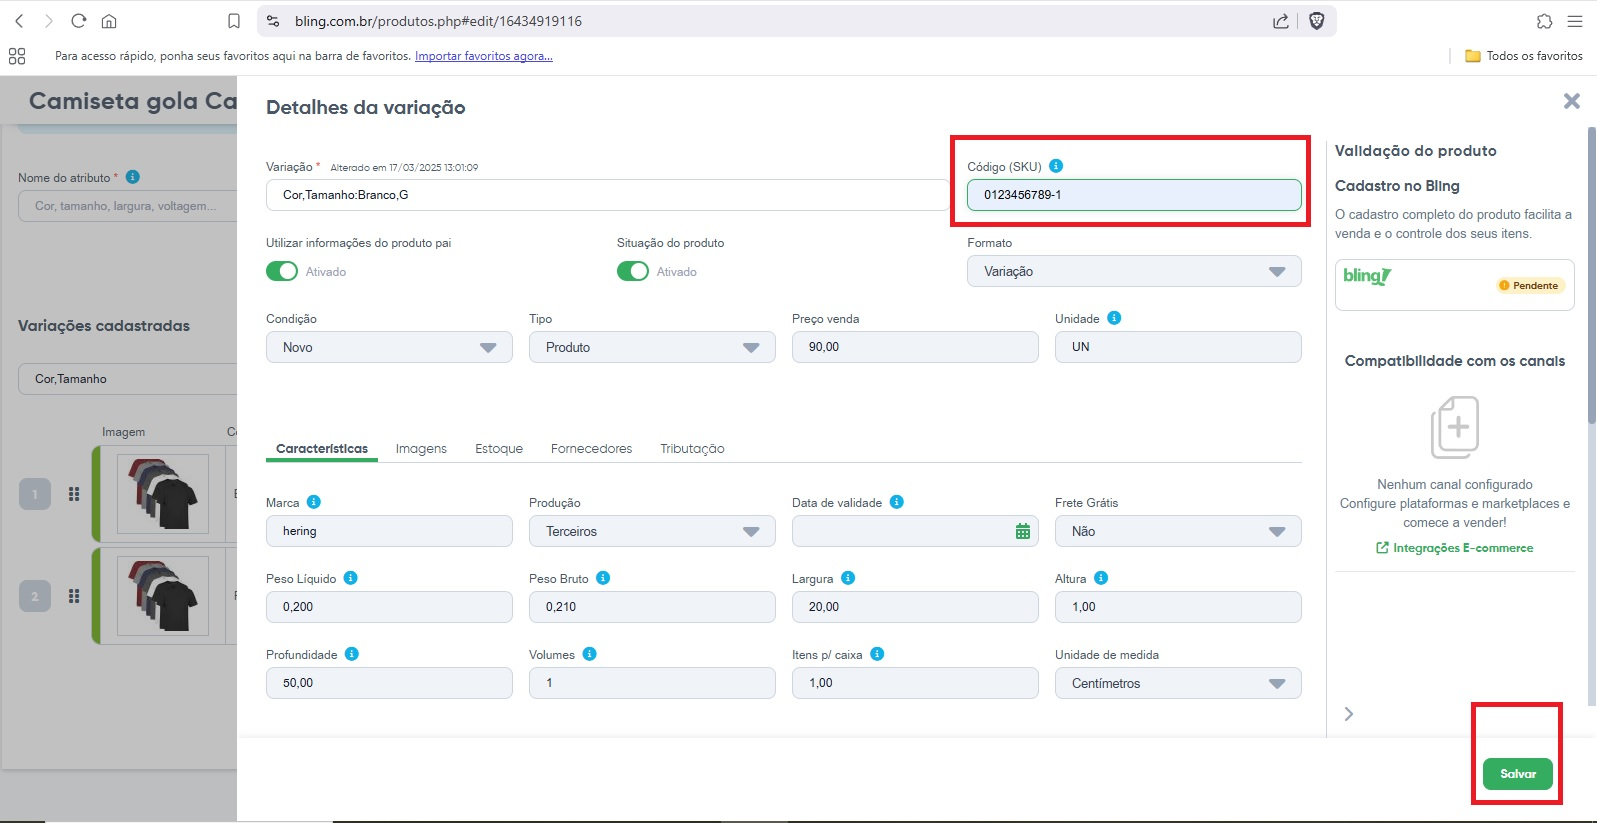
\includegraphics{images/np1/032-cadastro-produtos-variações-produto-inserir-código.jpg} 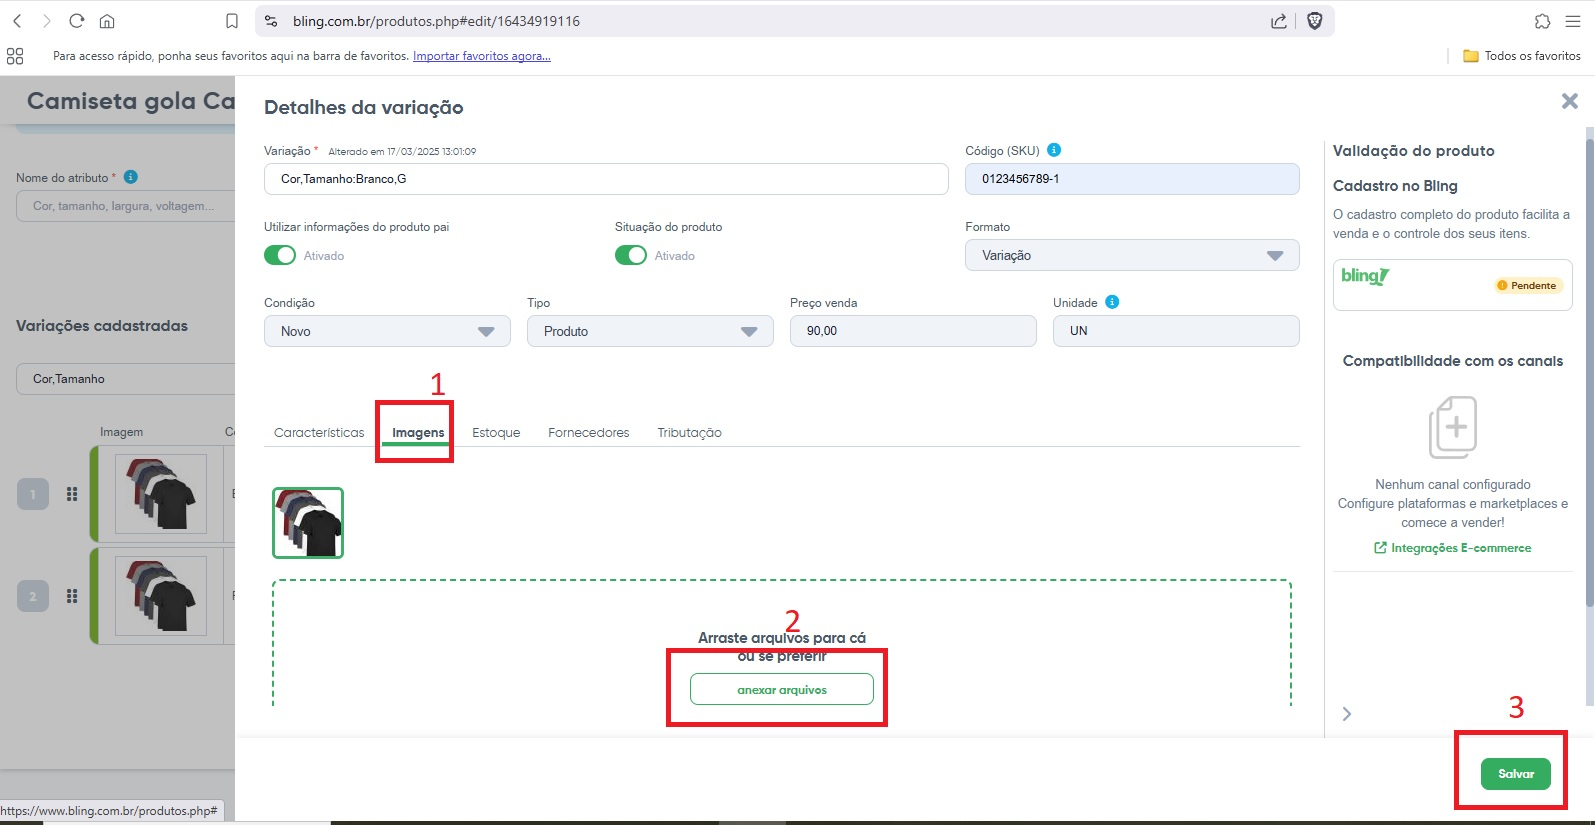
\includegraphics{images/np1/033-cadastro-produtos-variações-produto-inserir-imagem.jpg} \includegraphics{images/np1/034-cadastro-produtos-variações-produto.jpg}

\paragraph{Começar a cadastrar o estoque (Conceito de ``Módulo CONTROLE DE ESTOQUE'' dos ERPs)}\label{comeuxe7ar-a-cadastrar-o-estoque-conceito-de-muxf3dulo-controle-de-estoque-dos-erps}

\includegraphics{images/np1/035-bling-produto-cadastrado-sem-estoque.jpg} \includegraphics{images/np1/036-bling-estoque-produto-incluir.jpg} \includegraphics{images/np1/037-bling-estoque-produto-incluir-camiseta-preta.jpg} \includegraphics{images/np1/038-bling-estoque-produto-incluir-camiseta-preta-iniciar.jpg} \includegraphics{images/np1/039-bling-estoque-produto-incluir-camiseta-preta-feito.jpg} \includegraphics{images/np1/040-bling-estoque-produto-lançado.jpg} \includegraphics{images/np1/041-bling-cadastrar-cliente.jpg} \includegraphics{images/np1/042-bling-cadastrar-cliente-feito.jpg} \includegraphics{images/np1/043-bling-cadastrar-cliente-feito.jpg} \includegraphics{images/np1/044-bling-cadastrar-fornecedor-feito.jpg} \includegraphics{images/np1/045-bling-cadastrar-fornecedor-feito.jpg}

\subsubsection{Começar a cadastrar PDV (Ponto de Venda) da parte física da loja (Conceito de ``Módulo de vendas - PDV'' dos ERPs)}\label{comeuxe7ar-a-cadastrar-pdv-ponto-de-venda-da-parte-fuxedsica-da-loja-conceito-de-muxf3dulo-de-vendas---pdv-dos-erps}

\includegraphics{images/np1/046-bling-abrir-loja-fisica-frente-caixa.jpg} \includegraphics{images/np1/047-bling-abrir-loja-fisica-frente-caixa-ignorar-certificado.jpg} \includegraphics{images/np1/048-bling-abrir-loja-fisica-frente-caixa-cadastrar-loja-matriz.jpg} \includegraphics{images/np1/049-bling-abrir-loja-fisica-frente-caixa-cadastrar-loja-matriz.jpg} \includegraphics{images/np1/050-bling-abrir-loja-fisica-frente-caixa-ativo.jpg}

\subsection{Impantando o E-COMMERCE (parte virtual loja)}\label{impantando-o-e-commerce-parte-virtual-loja}

\subsection{ATIVE a PLATAFORMA DE E-COMMERCE}\label{ative-a-plataforma-de-e-commerce}

\subsubsection{cadastre a empresa do cliente na platafroma de e-commerce}\label{cadastre-a-empresa-do-cliente-na-platafroma-de-e-commerce}

\includegraphics{images/np1/051-nuvemshop-testar-loja-gratis.jpg} \includegraphics{images/np1/052-nuvemshop-cadastrar-loja-gratis.jpg} \includegraphics{images/np1/053-nuvemshop-testar-loja-gratis.jpg} \includegraphics{images/np1/054-nuvemshop-cadastrar-loja-gratis.jpg} \includegraphics{images/np1/055-nuvemshop-cadastrar-loja-gratis.jpg}

\subsubsection{cadastre as categorias de produtos na loja on-line}\label{cadastre-as-categorias-de-produtos-na-loja-on-line}

\includegraphics{images/np1/056-nuvemshop-cadastrar-categorias-produtos.jpg} \includegraphics{images/np1/057-nuvemshop-acessar-cadastro-categorias-produtos.jpg} \includegraphics{images/np1/058-nuvemshop-acessar-cadastro-categorias-produtos.jpg} \includegraphics{images/np1/059-nuvemshop-cadastrar-categorias-produtos.jpg} \includegraphics{images/np1/060-nuvemshop-cadastrar-subcategorias-produtos.jpg} \includegraphics{images/np1/061-nuvemshop-categorias-bling.jpg}

\subsubsection{mapeie o código das categorias de produtos na loja on-line para colocar no ERP depois}\label{mapeie-o-cuxf3digo-das-categorias-de-produtos-na-loja-on-line-para-colocar-no-erp-depois}

\includegraphics{images/np1/062-nuvemshop-obter-código-categorias.jpg} \includegraphics{images/np1/063-nuvemshop-obter-código-categorias.jpg} \includegraphics{images/np1/064-nuvemshop-categorias-nuvemshop-códigos.jpg} \includegraphics{images/np1/065-nuvemshop-visitar-loja-online.jpg} \includegraphics{images/np1/066-nuvemshop-visitar-loja-online.jpg} \includegraphics{images/np1/067-nuvemshop-visitar-loja-online.jpg}

\subsection{Inicie a amarração (integração) do e-commerce com o ERP (começando no e-commerce)}\label{inicie-a-amarrauxe7uxe3o-integrauxe7uxe3o-do-e-commerce-com-o-erp-comeuxe7ando-no-e-commerce}

\subsubsection{Instale o aplicativo (API) de conexão no e-commerce}\label{instale-o-aplicativo-api-de-conexuxe3o-no-e-commerce}

\includegraphics{images/np1/068-Conectar-nuvemshop-bling.jpg} \includegraphics{images/np1/069-Conectar-nuvemshop-bling.jpg} \includegraphics{images/np1/070-Conectar-nuvemshop-bling.jpg} \includegraphics{images/np1/071-Conectar-nuvemshop-bling.jpg}

\subsubsection{Instale o aplicativo (API) de conexão no ERP}\label{instale-o-aplicativo-api-de-conexuxe3o-no-erp}

\includegraphics{images/np1/072-Conectar-bling-nuvemshop.jpg} \includegraphics{images/np1/073-Conectar-bling-nuvemshop.jpg} \includegraphics{images/np1/074-Conectar-bling-nuvemshop-ajustes-finos.jpg} \includegraphics{images/np1/075-Conectar-bling-nuvemshop-ajustes-finos.jpg} \includegraphics{images/np1/076-Conectar-bling-nuvemshop-ajustes-finos-vendas.jpg} \includegraphics{images/np1/077-Conectar-bling-nuvemshop-ajustes-finos-vendas.jpg} \includegraphics{images/np1/078-Conectar-bling-nuvemshop-ajustes-feito.jpg}

\subsubsection{Faça agora o mapeamento do código das categorias do e-commerce no ERP}\label{fauxe7a-agora-o-mapeamento-do-cuxf3digo-das-categorias-do-e-commerce-no-erp}

\includegraphics{images/np1/079-Amarracao-Categorias-Ecommerce-ERP.jpg} \includegraphics{images/np1/080-Amarracao-Categorias-Ecommerce-ERP.jpg} \includegraphics{images/np1/081-Amarracao-Categorias-Ecommerce-ERP.jpg} \includegraphics{images/np1/082-Amarracao-Categorias-Ecommerce-ERP.jpg}

\subsubsection{Faça agora a exportação dos produtos}\label{fauxe7a-agora-a-exportauxe7uxe3o-dos-produtos}

\includegraphics{images/np1/083-Exportar-Bling-Nuvemshop.jpg} \includegraphics{images/np1/084-Exportar-Bling-Nuvemshop.jpg} \includegraphics{images/np1/085-Exportar-Bling-Nuvemshop.jpg} \includegraphics{images/np1/086-Exportar-Bling-Nuvemshop.jpg} \includegraphics{images/np1/087-Exportar-Bling-Nuvemshop.jpg} \includegraphics{images/np1/088-Exportar-Bling-Nuvemshop.jpg}

\subsubsection{Parabéns, hora de começar a testar seu e-commerce.}\label{parabuxe9ns-hora-de-comeuxe7ar-a-testar-seu-e-commerce.}

\includegraphics{images/np1/089-loja_virtual_com_produtos_carregados.jpg}

\subsection{INICIANDO O PROCESSO DE VENDA SIMULADA NO E-COMMERCE INTEGRADO AO ERP:}\label{iniciando-o-processo-de-venda-simulada-no-e-commerce-integrado-ao-erp}

\subsubsection{Configurar no e-commerce um ou mais MEIO(s) DE PAGAMENTO}\label{configurar-no-e-commerce-um-ou-mais-meios-de-pagamento}

No e-commerce (nuvemshop nesse caso) vá atá a aba de configuração.

\includegraphics{images/np1/090-loja_virtual_meio_de_pagamento1.jpg}

Procure pelo menu ``Meio de Pagamento''

\includegraphics{images/np1/091-loja_virtual_meio_de_pagamento2.jpg}

Aqui temos várias opções disponíveis para o dinheiro vir do comprador até a empresa (seu cliente) dona do site de e-commerce:

\begin{enumerate}
\def\labelenumi{\arabic{enumi}.}
\item
  Cartões de Débito ( Via ``mercado pago'', ``núvem pago'', ``Cielo'', ``Rede'' etc )
\item
  Cartões de Crédito ( Via ``mercado pago'', ``núvem pago'', ``Cielo'', ``Rede'' etc
\item
  Via boleto
\item
  Via PIX
\item
  (pesonalizado) Via troca de conversa whatsapp, onde manualmente o cliente termina a compra, pega a chave pix da loja virtual pelo whatsapp ou e-mail por exemplo, paga e envia o comprovante no whatsapp ou e-mail da loja virtual/e-commerce. Nessa modalidade, não há necessidade de se cadastrar em meios de pagamento, e portanto, não há cobrança de taxas pelos meios-de-pagamento. Utilizaremos esse método para nosso estudo de caso.
\end{enumerate}

Localize o meio de pagamento personalizado

\includegraphics{images/np1/092-loja_virtual_meio_de_pagamento3.jpg}

Ative esse tipo de meio-de-pagamento.

\includegraphics{images/np1/093-loja_virtual_meio_de_pagamento_personalizado.jpg}

Ative apenas a opção ``A combinar'' (referente a fazer a conferência de pagamento manualmente).

\includegraphics{images/np1/094-loja_virtual_meio_de_pagamento_personalizado_A_combinar.jpg}

\includegraphics{images/np1/095-loja_virtual_meio_de_pagamento_personalizado_A_combinar.jpg}

Pronto. Apenas confirme que seu meio de pagamento está configurado e ativado.

\includegraphics{images/np1/096-loja_virtual_meio_de_pagamento_personalizado_ativado.jpg}

\subsubsection{Simulação do comprador comprando uma camiseta}\label{simulauxe7uxe3o-do-comprador-comprando-uma-camiseta}

\includegraphics{images/np1/097-loja_virtual_iniciando_compra.jpg}

\includegraphics{images/np1/098-loja_virtual_iniciando_compra2.jpg}

\includegraphics{images/np1/099-loja_virtual_iniciando_compra3.jpg}

\includegraphics{images/np1/100-loja_virtual_iniciando_compra4.jpg}

\includegraphics{images/np1/101-loja_virtual_iniciando_compra5.jpg}

\includegraphics{images/np1/102-loja_virtual_iniciando_compra6.jpg}

\subsubsection{Aprovação manual da compra}\label{aprovauxe7uxe3o-manual-da-compra}

\paragraph{Cliente recebe status da compra (pedido e status de pagamento)}\label{cliente-recebe-status-da-compra-pedido-e-status-de-pagamento}

Neste ponto o comprador recebe um e-mail informando:

\begin{longtable}[]{@{}ll@{}}
\toprule\noalign{}
\endhead
\bottomrule\noalign{}
\endlastfoot
\textbf{Número do pedido} & No caso esse número é o \#100 \\
\textbf{Status do pagamento} & Informa que está aguardando pagamento \\
\end{longtable}

\includegraphics{images/np1/103-loja_virtual_cliente_email_confirmacao.jpg}

\paragraph{Cliente manda comprovante de pagamento}\label{cliente-manda-comprovante-de-pagamento}

\includegraphics{images/np1/104-loja_virtual_cliente_comprovante_pagamento.jpg}

\paragraph{parte 01 - liberação pedido de venda no e-commerce}\label{parte-01---liberauxe7uxe3o-pedido-de-venda-no-e-commerce}

\includegraphics{images/np1/105-loja_virtual_lberar_venda1.jpg}

\includegraphics{images/np1/106-loja_virtual_lberar_venda2.jpg}

\includegraphics{images/np1/107-loja_virtual_lberar_venda3.jpg}

\includegraphics{images/np1/108-loja_virtual_liberar_venda4.jpg}

\paragraph{parte 02 - Fechar venda no ERP ( dar baixa no estoque e lançamento de contas )}\label{parte-02---fechar-venda-no-erp-dar-baixa-no-estoque-e-lanuxe7amento-de-contas}

OBS: conforme combiando, por razões de limitações do estduo de caso, não vamos emitir nota fiscal para esta venda.

Acesse o módulo de vendas. Entre em pedidos de venda.

\includegraphics{images/np1/109-ERP_liberar_venda1.jpg}

Veja qu o sistema já puxou a venda do e-commerce, mas pelo processo estar no ``modo manual'', precisamos fazer o sistema:

\begin{longtable}[]{@{}
  >{\raggedright\arraybackslash}p{(\columnwidth - 2\tabcolsep) * \real{0.5000}}
  >{\raggedright\arraybackslash}p{(\columnwidth - 2\tabcolsep) * \real{0.5000}}@{}}
\toprule\noalign{}
\begin{minipage}[b]{\linewidth}\raggedright
Ações manuais sobre a venda
\end{minipage} & \begin{minipage}[b]{\linewidth}\raggedright
Descrição e importância
\end{minipage} \\
\midrule\noalign{}
\endhead
\bottomrule\noalign{}
\endlastfoot
1- Atualizar o estoque & De 2 camisetas pretas existentes na loja, 1 foi vendida, portanto restando apenas 1 para vender \\
2- Atualizar as contas & O valor da venda, sem o frente, foi de R\$ 90,00. Portanto entrou R\$ 90,00 nas contas a receber. \\
3- Fechar a venda dentro do ERP & Regra de ERP: para pode emitir nota fiscal e mandar embalar a camiseta, é preciso fechar o pedido primeiro. \\
\end{longtable}

Verifique o status atual da sua venda que foi recebida do e-commerce:

\includegraphics{images/np1/110-ERP_liberar_venda2.jpg}

Atualize o estoque seguindo os passos abaixo:

\includegraphics{images/np1/111-ERP_liberar_venda3.jpg}

Atualize as contas seguindo os passos abaixo:

\includegraphics{images/np1/112-ERP_liberar_venda4.jpg}

Feche a venda seguindo os passos abaixo

\includegraphics{images/np1/113-ERP_liberar_venda5.jpg}

Coloque uma observação (já que você fez o processo manualmente).

\includegraphics{images/np1/114-ERP_liberar_venda6.jpg}

Pronto, agora é só verificar a sua venda finalizada.

\includegraphics{images/np1/115-ERP_liberar_venda7.jpg}

Parabéns para você que chegou aqui!

Você implantou um e-commerce gerenciado por ERP para um cliente.

\section{CASO DE SUCESSO NO BRASIL DE UMA STARTUP, NESSE CASO ESPECÍFICAMENTE, DE I.A.}\label{caso-de-sucesso-no-brasil-de-uma-startup-nesse-caso-especuxedficamente-de-i.a.}

\subsection{Fundada por brasileiro, CrewAI capta R\$ 100M e atrai CEO da OpenAI}\label{fundada-por-brasileiro-crewai-capta-r-100m-e-atrai-ceo-da-openai}

A matéria completa está em \url{https://startups.com.br/negocios/fundada-por-brasileiro-crewai-capta-r-100m-e-atrai-ceo-da-openai/}

\subsection{CrewAI: Um guia com exemplos de sistemas de múltiplos agentes de IA}\label{crewai-um-guia-com-exemplos-de-sistemas-de-muxfaltiplos-agentes-de-ia}

Como testar a ferramenta crewai através dos pacotes python \texttt{crewai-tools\ crewai}

\url{https://www.datacamp.com/pt/tutorial/crew-ai}

\section{Lista de 100 Startups Brasileiras de Sucesso}\label{lista-de-100-startups-brasileiras-de-sucesso}

\begin{longtable}[]{@{}
  >{\centering\arraybackslash}p{(\columnwidth - 4\tabcolsep) * \real{0.2083}}
  >{\centering\arraybackslash}p{(\columnwidth - 4\tabcolsep) * \real{0.2500}}
  >{\raggedright\arraybackslash}p{(\columnwidth - 4\tabcolsep) * \real{0.5417}}@{}}
\toprule\noalign{}
\begin{minipage}[b]{\linewidth}\centering
\textbf{id}
\end{minipage} & \begin{minipage}[b]{\linewidth}\centering
\textbf{Nome}
\end{minipage} & \begin{minipage}[b]{\linewidth}\raggedright
Área de Atuação
\end{minipage} \\
\midrule\noalign{}
\endhead
\bottomrule\noalign{}
\endlastfoot
\textbf{1} & \textbf{Nubank} & Serviços financeiros digitais \\
\textbf{2} & \textbf{iFood} & Entrega de comida e mercado \\
\textbf{3} & \textbf{QuintoAndar} & Plataforma de aluguel e compra de imóveis \\
\textbf{4} & \textbf{Loft} & Compra e venda de imóveis \\
\textbf{5} & \textbf{Creditas} & Empréstimos com garantia \\
\textbf{6} & \textbf{Gympass} & Plataforma de bem-estar e atividades físicas \\
\textbf{7} & \textbf{MadeiraMadeira} & Venda online de móveis e artigos para casa \\
\textbf{8} & \textbf{VTEX} & Plataforma de comércio digital \\
\textbf{9} & \textbf{CargoX} & Plataforma de logística e transporte \\
\textbf{10} & \textbf{Neon} & Banco digital \\
\textbf{11} & \textbf{EBANX} & Processamento de pagamentos \\
\textbf{12} & \textbf{Hotmart} & Plataforma de produtos digitais \\
\textbf{13} & \textbf{Loggi} & Logística para e-commerce \\
\textbf{14} & \textbf{Wildlife Studios} & Desenvolvimento de jogos \\
\textbf{15} & \textbf{Stone} & Soluções de pagamento \\
\textbf{16} & \textbf{RD Station} & Automação de marketing e vendas \\
\textbf{17} & \textbf{Conta Azul} & Software de gestão para pequenas empresas \\
\textbf{18} & \textbf{Descomplica} & Educação online \\
\textbf{19} & \textbf{Facily} & E-commerce social \\
\textbf{20} & \textbf{Olist} & Plataforma para vendas online \\
\textbf{21} & \textbf{Docket} & Gestão de documentos \\
\textbf{22} & \textbf{Alice} & Plano de saúde \\
\textbf{23} & \textbf{Daki} & Supermercado online \\
\textbf{24} & \textbf{Hashdex} & Gestão de criptoativos \\
\textbf{25} & \textbf{Kavak} & Compra e venda de carros usados \\
\textbf{26} & \textbf{unico} & Identidade digital \\
\textbf{27} & \textbf{Buser} & Transporte rodoviário \\
\textbf{28} & \textbf{Pagar.me} & Soluções de pagamento online \\
\textbf{29} & \textbf{Rappi} & Entrega de diversos produtos \\
\textbf{30} & \textbf{Zé Delivery} & Entrega de bebidas \\
\textbf{31} & \textbf{Petlove} & Produtos e serviços para pets \\
\textbf{32} & \textbf{Sami} & Plano de saúde \\
\textbf{33} & \textbf{Kovi} & Aluguel de carros por assinatura \\
\textbf{34} & \textbf{Warren} & Plataforma de investimentos \\
\textbf{35} & \textbf{Liv Up} & Alimentação saudável \\
\textbf{36} & \textbf{Trybe} & Escola de programação \\
\textbf{37} & \textbf{Amaro} & E-commerce de moda \\
\textbf{38} & \textbf{Cortex} & Inteligência de dados \\
\textbf{39} & \textbf{Infracommerce} & Soluções para e-commerce \\
\textbf{40} & \textbf{Gupy} & Recrutamento e seleção \\
\textbf{41} & \textbf{Flash Benefícios} & Benefícios corporativos \\
\textbf{42} & \textbf{Méliuz} & Cashback e cupons \\
\textbf{43} & \textbf{Omie} & Software de gestão para PMEs \\
\textbf{44} & \textbf{Dr.~Consulta} & Clínicas populares \\
\textbf{45} & \textbf{Zenklub} & Saúde mental \\
\textbf{46} & \textbf{PicPay} & Carteira digital \\
\textbf{47} & \textbf{Creditas Auto} & Empréstimos com garantia de veículo \\
\textbf{48} & \textbf{99} & Aplicativo de mobilidade urbana \\
\textbf{49} & \textbf{C6 Bank} & Banco digital \\
\textbf{50} & \textbf{CloudWalk} & Pagamentos digitais \\
\textbf{51} & \textbf{Neon Pagamentos} & Banco digital \\
\textbf{52} & \textbf{Quero Educação} & Educação \\
\textbf{53} & \textbf{Loft} & Plataforma de compra e venda de imóveis \\
\textbf{54} & \textbf{Creditas} & Plataforma de empréstimos online \\
\textbf{55} & \textbf{Gympass} & Plataforma de bem-estar corporativo \\
\textbf{56} & \textbf{MadeiraMadeira} & E-commerce de produtos para casa \\
\textbf{57} & \textbf{VTEX} & Plataforma de e-commerce \\
\textbf{58} & \textbf{CargoX} & Plataforma de transporte de cargas \\
\textbf{59} & \textbf{Neon Pagamentos} & Banco digital \\
\textbf{60} & \textbf{EBANX} & Processamento de pagamentos \\
\textbf{61} & \textbf{Hotmart} & Plataforma de produtos digitais \\
\textbf{62} & \textbf{Loggi} & Logística para e-commerce \\
\textbf{63} & \textbf{Wildlife Studios} & Desenvolvimento de jogos \\
\textbf{64} & \textbf{Stone} & Soluções de pagamento \\
\textbf{65} & \textbf{RD Station} & Plataforma de automação de marketing \\
\textbf{66} & \textbf{Conta Azul} & Software de gestão para pequenas empresas \\
\textbf{67} & \textbf{Descomplica} & Educação online \\
\textbf{68} & \textbf{Facily} & Plataforma de compras online \\
\textbf{69} & \textbf{Olist} & Plataforma de vendas online \\
\textbf{70} & \textbf{Docket} & Plataforma de gestão de documentos \\
\textbf{71} & \textbf{Alice} & Plano de saúde \\
\textbf{72} & \textbf{Daki} & Supermercado online \\
\textbf{73} & \textbf{Hashdex} & Gestão de criptoativos \\
\textbf{74} & \textbf{Kavak} & Compra e venda de carros usados \\
\textbf{75} & \textbf{unico} & Plataforma de identidade digital \\
\textbf{76} & \textbf{Buser} & Transporte rodoviário \\
\textbf{77} & \textbf{Pagar.me} & Soluções de pagamento online \\
\textbf{78} & \textbf{Rappi} & Aplicativo de entrega \\
\textbf{79} & \textbf{Zé Delivery} & Entrega de bebidas \\
\textbf{80} & \textbf{Petlove} & E-commerce de produtos para pets \\
\textbf{81} & \textbf{Sami} & Plano de saúde \\
\textbf{82} & \textbf{Kovi} & Aluguel de carros por assinatura \\
\textbf{83} & \textbf{Warren} & Plataforma de investimentos \\
\textbf{84} & \textbf{Liv Up} & Plataforma de alimentação saudável \\
\textbf{85} & \textbf{Trybe} & Escola de programação \\
\textbf{86} & \textbf{Amaro} & E-commerce de moda \\
\textbf{87} & \textbf{Cortex} & Plataforma de inteligência de dados \\
\textbf{88} & \textbf{Infracommerce} & Soluções para e-commerce \\
\textbf{89} & \textbf{Gupy} & Plataforma de recrutamento e seleção \\
\textbf{90} & \textbf{Flash Benefícios} & Plataforma de benefícios corporativos \\
\textbf{91} & \textbf{Méliuz} & Plataforma de cashback e cupons \\
\textbf{92} & \textbf{Omie} & Software de gestão para pequenas empresas \\
\textbf{93} & \textbf{Dr.~Consulta} & Clínicas populares \\
\textbf{94} & \textbf{Zenklub} & Plataforma de saúde mental \\
\textbf{95} & \textbf{PicPay} & Carteira digital \\
\textbf{96} & \textbf{Creditas Auto} & Empréstimos com garantia de veículo \\
\textbf{97} & \textbf{Neon Pagamentos} & Banco digital \\
\textbf{98} & \textbf{99} & Aplicativo de mobilidade urbana \\
\textbf{99} & \textbf{C6 Bank} & Banco digital \\
\textbf{100} & \textbf{CloudWalk} & Pagamentos digitais \\
\end{longtable}

\chapter{INFRAESTRUTURA DE TIC}\label{infraestrutura-de-tic}

\section{Introdução:}\label{introduuxe7uxe3o-1}

No mundo da infraestrutura de TIC das empresas, diferentemente da área de desenvolvimento de software, é necessário conhecer e certificar-se em tecnologiasa e boas práticas de gestão departamental integrada ao negócio central (core business) da empresa.

A seguir, iremos conhecer as tecnologias e serviços de TIC presentes nos departamentos de tecnologia da informação das organizações em 2025, bem como as boas prtaicas de gestão para administrar tais departamentos.

\section{Componentes da Infraestrutura de TIC}\label{componentes-da-infraestrutura-de-tic}

Em uma empresa, a infraestrutura de TIC precisa de 3 elementos fundamentais para funcionar:

\begin{itemize}
\item
  Hardware;
\item
  Software;
\item
  Pessoas especializadas;
\end{itemize}

\subsection{Hardware}\label{hardware}

Fazem parte do cabedal de hadware das empresas:

\textbf{Estações de Trabalho} (WorkStations) - É um computador direcionado a atividades profissionais que, frequentemente, demandam bastante desempenho no processamento de dados;

\includegraphics[width=4.3125in,height=\textheight]{images/InfraEstrutura/hardware/01-estacao_de_trabalho.jpg}

\textbf{Computadores Pessoais} (Laptops e Desktops) - Um Computador Pessoal empresarial é um computador de mesa com capacidade dimensionada para uso em empresas e organizações visando tratar tarefas administrativas dos departamentos. O mesmo se aplica aos computadores portáteis empresariais (laptops);

\includegraphics{images/InfraEstrutura/hardware/02-desktop-laptop.jpg}

\textbf{Dispositivos móveis} (Smartphones e Tablets) - Os smartphones e tablets empresarias são aparelho celular fornecido por uma empresa para que os colaboradores usem no trabalho, normalmente customizados com configurações avançadas, como e-mail corporativo, aplicativos de gestão de projetos e CRM (Sistema de Relacionamento com Clientes) ;

\includegraphics{images/InfraEstrutura/hardware/04-tablet_lenovo.jpg}

\subsection{Redes de Computadores}\label{redes-de-computadores}

\begin{itemize}
\tightlist
\item
  \textbf{Roteadores:} Direcionam o tráfego de dados entre redes. Operam em camada de rede OSI ``3''. Podem ser \textbf{roteadores internos} à empresa (Roteadores Internos ao Sistema Autônomo de Roteamento) ou \textbf{roteadores de borda} (Roteadores Externos ao Sistema Autônomo de Roteamento).
\end{itemize}

\begin{figure}
\centering
\includegraphics{images/InfraEstrutura/Redes/roteador-cisco.jpg}
\caption{Roteador exclusivo CISCO de pequeno porte - Interno ao Sistema Autônomo (AS)}
\end{figure}

\begin{figure}
\centering
\includegraphics{images/InfraEstrutura/Redes/roteador-cisco-3900.jpg}
\caption{Roteador exclusivo CISCO de grande porte - Roteador de Borda - externo ao Sistema Autônomo (AS)}
\end{figure}

\begin{itemize}
\tightlist
\item
  \textbf{Switches:} Conectam dispositivos dentro de uma rede local da empresa (LAN - Local Area Network). camada de rede OSI ``2''
\end{itemize}

\begin{figure}
\centering
\includegraphics{images/InfraEstrutura/Redes/switch-cisco-3750x-48.jpg}
\caption{Comutador (Switch) de camada ``2'' de 48 portas energizáveis (PoE) para dados e telefonia IP}
\end{figure}

\begin{itemize}
\tightlist
\item
  \textbf{Firewalls:} Protegem a rede contra acessos não autorizados e ameaças externas.
\end{itemize}

\begin{figure}
\centering
\includegraphics{images/InfraEstrutura/Redes/firewall-PaloAlto-PA850.jpg}
\caption{Firewall da empresa Palo Alto modelo PA-850}
\end{figure}

\begin{itemize}
\item
  \textbf{Pontos de Acesso Wi-Fi:} Permitem a conexão sem fio à rede. camada de rede OSI ``2''

  Os pontos de acesso de rede sem fio (WI-FI) formam uma grande célula wi-fi na empresa. A célula, tal qual um siwitch virtual, tem apenas a função de conectar os dispositivos, geralmente os dispositivos móveis, a rede local da empresa (LAN - Local Area Network).
\end{itemize}

\href{Pontos\%20de\%20Acesso\%20CISCO}{\includegraphics{images/InfraEstrutura/Redes/Ponto_De_Acesso-cisco.jpg}}

\begin{itemize}
\tightlist
\item
  \textbf{Cabos e Conectores:} A infraestrutura física para conectar os dispositivos. camada de rede OSI ``1''
\end{itemize}

\includegraphics[width=4.54167in,height=\textheight]{images/InfraEstrutura/Redes/cabos.jpg}

\subsection{Software}\label{software}

\subsubsection{Sistemas Operacionais}\label{sistemas-operacionais}

\begin{longtable}[]{@{}
  >{\centering\arraybackslash}p{(\columnwidth - 0\tabcolsep) * \real{1.0072}}@{}}
\toprule\noalign{}
\endhead
\bottomrule\noalign{}
\endlastfoot
\begin{minipage}[t]{\linewidth}\centering
\begin{center}
\includegraphics{images/InfraEstrutura/software/so.jpg}

Windows Linux MacOS FreeBSD NetBSD OpenBSD
\end{center}
\end{minipage} \\
\textbf{Sistemas Operacionais} são softwares fundamentais que gerenciam o hardware e os recursos do sistema. Exemplos de Sistemas Operacionais

\textbf{Microsoft Windows}

\textbf{Distribuições Linux}

\textbf{Apple MacOS}

\textbf{Unix FreeBSD}

\textbf{Unix NetBSD}

\textbf{Unix OpenBSD} \\
\end{longtable}

\subsubsection{Aplicações Empresariais}\label{aplicauxe7uxf5es-empresariais}

\begin{longtable}[]{@{}
  >{\centering\arraybackslash}p{(\columnwidth - 0\tabcolsep) * \real{1.0119}}@{}}
\toprule\noalign{}
\endhead
\bottomrule\noalign{}
\endlastfoot
\includegraphics{images/InfraEstrutura/software/erps.jpg} \\
\textbf{Aplicações Empresariais} são softwares utilizados para as atividades de negócio

(ex: ERP, CRM, sistemas de gestão de RH, sistemas de contabilidade).

\textbf{ERP BLING}

\textbf{ERP SAP}

\textbf{ERP TOTVS}

\textbf{ERP LINX} \\
\end{longtable}

\subsubsection{Softwares de Produtividade}\label{softwares-de-produtividade}

\begin{longtable}[]{@{}
  >{\centering\arraybackslash}p{(\columnwidth - 0\tabcolsep) * \real{1.0067}}@{}}
\toprule\noalign{}
\endhead
\bottomrule\noalign{}
\endlastfoot
\begin{minipage}[t]{\linewidth}\centering
\begin{center}
\includegraphics{images/InfraEstrutura/software/MS-Office.jpg}

Microsoft Office - Word Excel Powerpoint Teams Visio Edge Forms Publisher Access
\end{center}
\end{minipage} \\
\textbf{Software de Produtividade} são ferramentas para criação de documentos, planilhas, apresentações, e-mail (ex: Microsoft Office, Google Workspace). \\
\end{longtable}

\subsubsection{Softwares de Segurança}\label{softwares-de-seguranuxe7a}

\begin{longtable}[]{@{}
  >{\centering\arraybackslash}p{(\columnwidth - 0\tabcolsep) * \real{1.0046}}@{}}
\toprule\noalign{}
\endhead
\bottomrule\noalign{}
\endlastfoot
\begin{minipage}[t]{\linewidth}\centering
\begin{center}
\includegraphics{images/InfraEstrutura/software/seguranca.jpg}

Karspersky Norton Suricata IPTables PF Nmap Wireshark
\end{center}
\end{minipage} \\
\textbf{Software de Segurança} é uma categoria de software onde se enquadram os antivírus, anti-malware, sistemas de detecção de intrusão (IDS), sistemas de prevenção de intrusão (IPS). Exemplos de Softwares de Segurança

\textbf{Karspersky (Anti-vírus)}

\textbf{Norton (Anti-vírus)}

\textbf{Suricata (IDS - detector de Intrusão)}

\textbf{IPTables (Firewall nativo do Linux)}

\textbf{PF (Firewall nativo do Unix FreeBSD)}

\textbf{NMAP (Mapeador de portas TCP/IP)}

\textbf{Wireshark (Farejador - sniffer - de pacotes de rede)} \\
\end{longtable}

\subsubsection{Softwares de Gerenciamento de Rede}\label{softwares-de-gerenciamento-de-rede}

\begin{longtable}[]{@{}
  >{\centering\arraybackslash}p{(\columnwidth - 0\tabcolsep) * \real{1.0082}}@{}}
\toprule\noalign{}
\endhead
\bottomrule\noalign{}
\endlastfoot
\begin{minipage}[t]{\linewidth}\centering
\begin{center}
\includegraphics{images/InfraEstrutura/software/monitoramento.jpg}

SolarWinds Nagios Zabbix Cacti
\end{center}
\end{minipage} \\
\textbf{Software de Gerenciamento de Rede} é uma categoria deferramentas para monitorar e gerenciar a infraestrutura de rede. \\
\end{longtable}

\subsubsection{Sistemas de Gerenciamento de Banco de Dados (SGBDs)}\label{sistemas-de-gerenciamento-de-banco-de-dados-sgbds}

\begin{longtable}[]{@{}
  >{\raggedright\arraybackslash}p{(\columnwidth - 0\tabcolsep) * \real{1.0071}}@{}}
\toprule\noalign{}
\endhead
\bottomrule\noalign{}
\endlastfoot
\begin{minipage}[t]{\linewidth}\raggedright
\begin{itemize}
\tightlist
\item
  \textbf{Bancos de Dados:} Sistemas para armazenar e gerenciar grandes volumes de dados de forma organizada (ex: SQL Server, Oracle, MySQL).
\end{itemize}
\end{minipage} \\
\end{longtable}

\begin{longtable}[]{@{}
  >{\raggedright\arraybackslash}p{(\columnwidth - 2\tabcolsep) * \real{0.6933}}
  >{\centering\arraybackslash}p{(\columnwidth - 2\tabcolsep) * \real{0.3067}}@{}}
\toprule\noalign{}
\endhead
\bottomrule\noalign{}
\endlastfoot
\textbf{Paradigma relacional}

\includegraphics[width=2.16667in,height=\textheight]{images/clipboard-3269919173.png} & Postgres

Mysql

Microsoft SQL Server

IBM DB2

Oracle \\
\end{longtable}

\begin{longtable}[]{@{}
  >{\raggedright\arraybackslash}p{(\columnwidth - 2\tabcolsep) * \real{0.5417}}
  >{\centering\arraybackslash}p{(\columnwidth - 2\tabcolsep) * \real{0.2778}}@{}}
\toprule\noalign{}
\endhead
\bottomrule\noalign{}
\endlastfoot
\textbf{Paradigma não-relacional}

\includegraphics{images/clipboard-1618144074.png} & Cassandra

MongoDB \\
\end{longtable}

\begin{longtable}[]{@{}
  >{\raggedright\arraybackslash}p{(\columnwidth - 2\tabcolsep) * \real{0.5417}}
  >{\centering\arraybackslash}p{(\columnwidth - 2\tabcolsep) * \real{0.2778}}@{}}
\toprule\noalign{}
\endhead
\bottomrule\noalign{}
\endlastfoot
\textbf{Paradigma Grafo}

\includegraphics{images/clipboard-2057319963.png} & neo4J \\
\end{longtable}

\begin{longtable}[]{@{}
  >{\raggedright\arraybackslash}p{(\columnwidth - 2\tabcolsep) * \real{0.7222}}
  >{\centering\arraybackslash}p{(\columnwidth - 2\tabcolsep) * \real{0.2639}}@{}}
\toprule\noalign{}
\endhead
\bottomrule\noalign{}
\endlastfoot
\textbf{Paradigma Hierárquico}

\includegraphics[width=3.625in,height=\textheight]{images/clipboard-1964387230.png} & Active Directory

OpenLDAP \\
\end{longtable}

\subsubsection{Middleware: Software que permite a comunicação e a troca de dados entre diferentes aplicações.}\label{middleware-software-que-permite-a-comunicauxe7uxe3o-e-a-troca-de-dados-entre-diferentes-aplicauxe7uxf5es.}

\begin{longtable}[]{@{}
  >{\centering\arraybackslash}p{(\columnwidth - 2\tabcolsep) * \real{0.3611}}
  >{\centering\arraybackslash}p{(\columnwidth - 2\tabcolsep) * \real{0.3889}}@{}}
\toprule\noalign{}
\endhead
\bottomrule\noalign{}
\endlastfoot
\textbf{Tipo de MiddleWare} & \textbf{Exemplo de Middleware} \\
Filas de Mensagens & Apache Kafka

RabbitMQ \\
\end{longtable}

\begin{longtable}[]{@{}
  >{\centering\arraybackslash}p{(\columnwidth - 2\tabcolsep) * \real{0.4306}}
  >{\centering\arraybackslash}p{(\columnwidth - 2\tabcolsep) * \real{0.3889}}@{}}
\toprule\noalign{}
\endhead
\bottomrule\noalign{}
\endlastfoot
\textbf{Tipo de MiddleWare} & \textbf{Exemplo de Middleware} \\
Enterprise Service BUS (ESB) & Apache Camel

Mulesoft \\
\end{longtable}

\begin{longtable}[]{@{}
  >{\centering\arraybackslash}p{(\columnwidth - 2\tabcolsep) * \real{0.3611}}
  >{\centering\arraybackslash}p{(\columnwidth - 2\tabcolsep) * \real{0.3889}}@{}}
\toprule\noalign{}
\endhead
\bottomrule\noalign{}
\endlastfoot
\textbf{Tipo de MiddleWare} & \textbf{Exemplo de Middleware} \\
APIs Gateways & KONG

TYK \\
\end{longtable}

\begin{longtable}[]{@{}
  >{\centering\arraybackslash}p{(\columnwidth - 2\tabcolsep) * \real{0.5139}}
  >{\centering\arraybackslash}p{(\columnwidth - 2\tabcolsep) * \real{0.3889}}@{}}
\toprule\noalign{}
\endhead
\bottomrule\noalign{}
\endlastfoot
\textbf{Tipo de MiddleWare} & \textbf{Exemplo de Middleware} \\
Middleware de Banco de Dados (ORM) & Hibernate (java)

SQLAlchemy (python)

soci (c++) \\
\end{longtable}

\begin{longtable}[]{@{}
  >{\centering\arraybackslash}p{(\columnwidth - 2\tabcolsep) * \real{0.3611}}
  >{\centering\arraybackslash}p{(\columnwidth - 2\tabcolsep) * \real{0.3889}}@{}}
\toprule\noalign{}
\endhead
\bottomrule\noalign{}
\endlastfoot
\textbf{Tipo de MiddleWare} & \textbf{Exemplo de Middleware} \\
Computação Distribuida & CORBA

JAVA RMI \\
\end{longtable}

\subsubsection{Softwares de Virtualização}\label{softwares-de-virtualizauxe7uxe3o}

\begin{longtable}[]{@{}
  >{\centering\arraybackslash}p{(\columnwidth - 0\tabcolsep) * \real{1.0081}}@{}}
\toprule\noalign{}
\endhead
\bottomrule\noalign{}
\endlastfoot
\textbf{Software de Virtualização:} Permite executar múltiplos sistemas operacionais e aplicações em um único servidor físico.

\includegraphics{images/InfraEstrutura/virtualização/virtualizacao.jpg} \\
Oracle Virtualbox (gratuito)

Microsoft Hyper-V

VMWARE Wokstation

GNU QEMU (emulador)

Linux KVM (Módulo do kernel) \\
\end{longtable}

\subsubsection{Softwares de Backup e Recuperação}\label{softwares-de-backup-e-recuperauxe7uxe3o}

\begin{longtable}[]{@{}
  >{\centering\arraybackslash}p{(\columnwidth - 2\tabcolsep) * \real{0.7267}}
  >{\raggedright\arraybackslash}p{(\columnwidth - 2\tabcolsep) * \real{0.2733}}@{}}
\toprule\noalign{}
\endhead
\bottomrule\noalign{}
\endlastfoot
\textbf{Sistemas de Backup e Recuperação:} Software para automatizar e gerenciar os processos de backup e restauração de dados. & \includegraphics{images/InfraEstrutura/backup/backup.jpg} \\
\end{longtable}

\subsection{Serviços de TIC}\label{serviuxe7os-de-tic}

\begin{longtable}[]{@{}
  >{\raggedright\arraybackslash}p{(\columnwidth - 4\tabcolsep) * \real{0.1330}}
  >{\raggedright\arraybackslash}p{(\columnwidth - 4\tabcolsep) * \real{0.6491}}
  >{\raggedright\arraybackslash}p{(\columnwidth - 4\tabcolsep) * \real{0.2156}}@{}}
\caption{Serviços de TIC}\tabularnewline
\toprule\noalign{}
\begin{minipage}[b]{\linewidth}\raggedright
Tipo de Serviço Corporativo
\end{minipage} & \begin{minipage}[b]{\linewidth}\raggedright
Descrição
\end{minipage} & \begin{minipage}[b]{\linewidth}\raggedright
Softwares servidores do serviço
\end{minipage} \\
\midrule\noalign{}
\endfirsthead
\toprule\noalign{}
\begin{minipage}[b]{\linewidth}\raggedright
Tipo de Serviço Corporativo
\end{minipage} & \begin{minipage}[b]{\linewidth}\raggedright
Descrição
\end{minipage} & \begin{minipage}[b]{\linewidth}\raggedright
Softwares servidores do serviço
\end{minipage} \\
\midrule\noalign{}
\endhead
\bottomrule\noalign{}
\endlastfoot
Correio eletrônico - E-Mail & Método de comunicação digital que permite o envio e recebimento de mensagens através da internet;

Softwares que implantam o serviço eletrônico são o \textbf{postfix, microsoft exchange, dovecot e o smtpd}; & \includegraphics{images/InfraEstrutura/servicos/e-mail/e-mail.jpg} \\
Compartilhamento de Arquivos & Permite aos usuários armazenar, acessar e distribuir arquivos digitais pela internet;

Softwares que implantam o serviço eletrônico são o \textbf{File Server do Windows, Samba (Linux), NFS (Linux e Unix)}; & \includegraphics{images/InfraEstrutura/servicos/compartilhamento-arquivos/compartilhamento-arquivos.jpg} \\
Compartilhamento de Impressoras & Permite que vários computadores em uma rede corporativa utilizem uma única impressora;

Softwares que implantam o serviço de impressão na rede são \textbf{CUPS (linux) e o Spool de Impressão do Windows}; & \includegraphics{images/InfraEstrutura/servicos/compartilhamento-impressao/impressao.jpg} \\
Serviço de Nomes de Domínio - DNS & É essencialmente a ``lista telefônica'' da internet. Ele traduz nomes de domínio amigáveis (como ``\href{https://www.google.com/search?q=google.com}{google.com}'') em endereços IP numéricos (como ``172.217.160.142''), que os computadores usam para se comunicar entre si.

Softwares que implantam o serviço de nomes de domínio na rede são \textbf{Bind (Linux) e o Active Directory (Windows)}; & \includegraphics{images/InfraEstrutura/servicos/servicos-nomeacao-dominio/nomes.jpg} \\
Gerenciamento de usuários da rede corporativa & Um serviço de gerenciamento de usuários de rede corporativa, também conhecido como domínio, é um sistema centralizado que permite aos administradores de TI controlar e gerenciar o acesso de usuários e recursos em uma rede corporativa;

Softwares que implantam o serviço de nomes de domínio na rede são \textbf{OpenLdap (Linux) e o Active Directory (Windows)}; & \includegraphics{images/InfraEstrutura/servicos/gestao-usuarios/gestao-usuarios.jpg} \\
Gerenciamento de páginas web e publicações corporativas & Um serviço de publicação de informações e documentos visando a propagação de informações internas e a colaboração entre equipes.

Softwares que implantam o serviço de páginas web e publicações corporativas são o servidor web \textbf{Apache (Linux e Unix),} o servidor web \textbf{NGINX (Linux e Unix)}, o \textbf{IIS} \textbf{(Internet Information Service)} da Microsoft e, mais recentemente, o \textbf{seviço Sharepoint} da Microsoft; & \includegraphics{images/InfraEstrutura/servicos/web/web.jpg} \\
\end{longtable}

\section{Gestão do Departamento de TIC nas empresas}\label{gestuxe3o-do-departamento-de-tic-nas-empresas}

\subsection{ITSM}\label{itsm}

A Gestão de Serviços de Informática chamada (GSTI) ou, no inglês, ITSM (IT Service Management) tem por objetivo prover um serviço de TI com qualidade e alinhado às necessidades do negócio, buscando redução de custos a longo prazo.

Nos últimos 40 anos, tem-se reunido boas práticas de Gestão de Serviços de Informática chamada ao ponto de criar ``bibliotecas'', ou seja, coleções de boas práticas. Vejamos as duas mais famosas:

\subsubsection{ITIL (Information Technology Infrastructure Library)}\label{itil-information-technology-infrastructure-library}

O ITIL (Information Technology Infrastructure Library) é um conjunto de melhores práticas para o gerenciamento de serviços de Tecnologia da Informação (TI). Ele fornece um framework abrangente e flexível que as organizações podem usar para alinhar seus serviços de TI com as necessidades de seus negócios. O ITIL ajuda as empresas a otimizar seus processos de TI, melhorar a qualidade dos serviços, reduzir custos e aumentar a satisfação do cliente.

Atualmente, a AXELOS é a proprietária do ITIL e responsável por sua evolução e pelas certificações relacionadas.

\includegraphics{images/InfraEstrutura/ITIL/Linha_do_Tempo.jpg}

Para dar uma noção sobre melhores práticas de gestão de processos de TIC, utilizaremos o framework ITIL em sua versão 2 (2001), uma vez que o mesmo possui apenas 10 processos de Gestão de TIC divididos em dois grupos chamdos disciplinas ITIL.

\paragraph{Processos ITIL Versão 2 (2001)}\label{processos-itil-versuxe3o-2-2001}

\begin{longtable}[]{@{}
  >{\centering\arraybackslash}p{(\columnwidth - 2\tabcolsep) * \real{0.4828}}
  >{\centering\arraybackslash}p{(\columnwidth - 2\tabcolsep) * \real{0.5172}}@{}}
\toprule\noalign{}
\begin{minipage}[b]{\linewidth}\centering
Grupo de Processos (Disciplina ITIL v2)
\end{minipage} & \begin{minipage}[b]{\linewidth}\centering
Processos
\end{minipage} \\
\midrule\noalign{}
\endhead
\bottomrule\noalign{}
\endlastfoot
\textbf{``GRUPO'' SUPORTE A SERVIÇO} & 01- Gestão de Incidentes

02- Gestão de Problemas

03- Gestão de Mudanças

04- Gestão de Liberação

05- Gestão Configuração \\
\textbf{``GRUPO'' ENTREGA DE SERVIÇO} & 06- Gestão de Nível de Serviço

07- Gestão de Disponibilidade

08- Gestão de Capacidade

09- Gestão de Continuidade de Serviços TIC

10- Gestão Financeira para Serviços de TIC \\
\end{longtable}

\paragraph{Processos do grupo SUPORTE A SERVIÇOS DE TIC}\label{processos-do-grupo-suporte-a-serviuxe7os-de-tic}

O ITIL descreve melhores práticas para gestão de serviços de TIC. A Disciplina (agrupamento) de Suporte ao Serviço e a Disciplina (agrupamento) de Fornecimento de serviço combinadas oferecem o recurso de \textbf{Gerenciamento de Serviço de TIC} a uma organização. Inter-relacionamentos complexos entre todas as dez disciplinas do Gerenciamento de Serviços interagem para garantir que a infraestrutura de TI forneça um alto nível de serviço aos negócios.

\subparagraph{01- Gestão de Incidentes}\label{gestuxe3o-de-incidentes}

\includegraphics{images/InfraEstrutura/ITIL/01-Gerencia_de_Incidentes-01.jpg}

\includegraphics{images/InfraEstrutura/ITIL/01-Gerencia_de_Incidentes-2.jpg}

O processo ``\textbf{Service Desk e Gerenciamento de Incidentes}'' visa restaurar os Serviços de TI para seus Níveis de Serviço definidos o mais rápido possível O processo também é responsável por receber e processar Solicitações de Serviço, por auxiliar os usuários e por coordenar a Resolução de Incidentes com Grupos de Suporte Especializados. Ao longo do processo, os usuários são informados em intervalos regulares sobre o status de seus incidentes.

\subparagraph{02- Gestão de Problemas}\label{gestuxe3o-de-problemas}

\includegraphics{images/InfraEstrutura/ITIL/02-Gerencia_de_Problemas.jpg}

O objetivo do \textbf{Processo de Gerenciamento de Problemas} é resolver a causa raiz dos Incidentes e evitar a recorrência de Incidentes relacionados a esses erros. Ele fornece Gerenciamento de Incidentes com Correções Temporárias (Soluções) e Soluções Permanentes para Erros Conhecidos. O Gerenciamento Proativo de Problemas identifica e resolve Problemas antes que os Incidentes ocorram, por exemplo, analisando tendências no Uso de Serviços de TI ou investigando Incidentes históricos.

\subparagraph{03- Gestão de Mudanças}\label{gestuxe3o-de-mudanuxe7as}

\includegraphics{images/InfraEstrutura/ITIL/03-Gerencia_de_Mudanças.jpg}

No \textbf{Processo de Gerenciamento de Mudanças}, todas as alterações na infraestrutura de TI e seus componentes (Itens de Configuração) são autorizadas e documentadas, a fim de garantir que os efeitos de interrupção na operação em execução sejam reduzidos ao mínimo. As etapas de implementação são planejadas e comunicadas, a fim de reconhecer possíveis efeitos colaterais o mais cedo possível. O Gerente de Mudanças e (para Mudanças de maior alcance) o Conselho Consultivo de Mudanças (CAB) são responsáveis por isso. Existe um procedimento específico para emergências, lidando com Mudanças Urgentes.

\subparagraph{04- Gestão de Liberação}\label{gestuxe3o-de-liberauxe7uxe3o}

\includegraphics{images/InfraEstrutura/ITIL/04-gerencia_de_liberação-02.jpg}

\includegraphics{images/InfraEstrutura/ITIL/04-Gerencia_de_Liberação-01.jpg}

O \textbf{Processo de Liberação de Mudanças} é responsável pela implementação de mudanças aprovadas na Infraestrutura de TI, para que estas sejam realizadas de forma eficaz, segura e verificável. As tarefas deste processo incluem planejamento, monitoramento e implementação dos respectivos \emph{Rollouts} ou \emph{Rollins} em coordenação com o Gerenciamento de Mudanças anteriormente citada.

\subparagraph{05- Gestão Configuração}\label{gestuxe3o-configurauxe7uxe3o}

\includegraphics{images/InfraEstrutura/ITIL/05-Gerencia_de_configuração.jpg}

As informações sobre Infraestrutura e Serviços necessárias para o Gerenciamento de Serviços de TI são disponibilizadas pelo Gerenciamento de Configuração. As alterações são documentadas e o status atualizado das informações é verificado regularmente. Com isso, informações atualizadas e históricas sobre os Itens de Configuração (CIs) estão continuamente disponíveis no Banco de Dados de Gerenciamento de Configuração (CMDB).

\paragraph{Processos do grupo ENTREGA DE SERVIÇOS DE TIC}\label{processos-do-grupo-entrega-de-serviuxe7os-de-tic}

\subparagraph{06- Gestão de Nível de Serviço}\label{gestuxe3o-de-nuxedvel-de-serviuxe7o}

\includegraphics[width=4.01042in,height=\textheight]{images/InfraEstrutura/ITIL/06-Gerencia_de_Nivel_de_Serviço.jpg}

O Gerenciamento de Nível de Serviço tem as tarefas de manter o Catálogo de Serviços da Organização de TI e alcançar acordos vinculativos para Desempenho de Serviços internos e externos. Na interface com o cliente, os Contratos de Nível de Serviço são acordados. O Gerente de Nível de Serviço é responsável pelo monitoramento dos parâmetros de qualidade acordados e, quando necessário, recorre a contramedidas. A prestação adequada de Serviços de TI internos é assegurada através de Acordos de Nível Operacional e Contratos de Apoio (OLAs/UCs).

\subparagraph{07- Gestão de Disponibilidade}\label{gestuxe3o-de-disponibilidade}

\includegraphics{images/InfraEstrutura/ITIL/07-gerenciamento_de_disponibilidade.jpg}

O Gerenciamento de Disponibilidade permite que as Organizações de TI sustentem a disponibilidade da infraestrutura de TI para atender aos Níveis de Serviço acordados definidos nos SLAs. Ele monitora constantemente os níveis de disponibilidade alcançados e, quando necessário, realiza medidas corretivas.

\subparagraph{08- Gestão de Capacidade}\label{gestuxe3o-de-capacidade}

\includegraphics{images/InfraEstrutura/ITIL/08-Gestao_de_capacidade.jpg}

O Gerenciamento de Capacidade suporta a provisão ideal e econômica de Serviços de TI, ajudando as Organizações de TI a combinar seus Recursos de TI (Software, Hardware, Recursos Humanos) com as necessidades de negócios. O processo envolve estimativas de demanda futura, que são a base para o planejamento de necessidades futuras de capacidade, resultando no Plano de Capacidade.

\subparagraph{09- Gestão de Continuidade de Serviços TIC}\label{gestuxe3o-de-continuidade-de-serviuxe7os-tic}

\includegraphics{images/InfraEstrutura/ITIL/09-Gestao_de_Continuidade_de_servicos_deTI.jpg}

O Gerenciamento de Continuidade de Serviço de TI define e planeja todas as medidas e processos para eventos imprevistos de desastre. A análise regular de vulnerabilidades, ameaças e riscos representa uma base para precauções adequadas.

\subparagraph{10- Gestão Financeira para Serviços de TI}\label{gestuxe3o-financeira-para-serviuxe7os-de-ti}

\includegraphics{images/InfraEstrutura/ITIL/10-Gestao_Financeira_servicos_TI.jpg}

O Gerenciamento Financeiro para Serviços de TI garante o uso mais econômico dos recursos financeiros de TI e cobra dos clientes pela prestação de Serviços de TI. Durante este período, deve ser alcançada uma relação equilibrada entre qualidade e custos, tendo simultaneamente em conta os requisitos do cliente. A realização do planeamento orçamental regular e o apuramento dos meios financeiros aprovados é também uma das tarefas da Gestão Financeira.

\section{Principais Certificações de TIC para analistas de infraestrutura iniciando na área em 2025:}\label{principais-certificauxe7uxf5es-de-tic-para-analistas-de-infraestrutura-iniciando-na-uxe1rea-em-2025}

\begin{longtable}[]{@{}
  >{\raggedright\arraybackslash}p{(\columnwidth - 6\tabcolsep) * \real{0.0619}}
  >{\raggedright\arraybackslash}p{(\columnwidth - 6\tabcolsep) * \real{0.3021}}
  >{\raggedright\arraybackslash}p{(\columnwidth - 6\tabcolsep) * \real{0.3058}}
  >{\raggedright\arraybackslash}p{(\columnwidth - 6\tabcolsep) * \real{0.3265}}@{}}
\toprule\noalign{}
\begin{minipage}[b]{\linewidth}\raggedright
Característica
\end{minipage} & \begin{minipage}[b]{\linewidth}\raggedright
ITIL® 4 Foundation
\end{minipage} & \begin{minipage}[b]{\linewidth}\raggedright
COBIT® 2019 Foundation
\end{minipage} & \begin{minipage}[b]{\linewidth}\raggedright
Cisco Certified Network Associate (CCNA)
\end{minipage} \\
\midrule\noalign{}
\endhead
\bottomrule\noalign{}
\endlastfoot
Organização & PeopleCert (em nome da AXELOS) & ISACA® & Cisco Systems, Inc. \\
Área Principal & Gerenciamento de Serviços de TI (ITSM) & Governança e Gestão de TI (EGIT) & Redes de Computadores \\
Foco & Melhores práticas para entregar e suportar serviços de TIC de forma eficaz e eficiente. Foco no valor para o negócio. & Framework para alinhar a TIC com os objetivos de negócio, gerenciando riscos e recursos de forma otimizada. & Instalação, configuração, operação e troubleshooting de redes (switches e roteadores). Fundamentos de segurança e automação de redes. \\
Público-Alvo & Profissionais de TI em geral (suporte, operações, desenvolvimento, gestão), gerentes de projeto, analistas de negócio. & Auditores de TI, gerentes de TI, profissionais de risco, conformidade (compliance) e segurança da informação, consultores. & Técnicos de rede, administradores de rede, engenheiros de rede juniores, técnicos de suporte com foco em infraestrutura. \\
Nível & Fundamental / Iniciante & Fundamental / Iniciante & Associado / Iniciante-Intermediário (bastante técnico) \\
Principais Conceitos Abordados & Sistema de Valor de Serviço (SVS), 4 Dimensões do Gerenciamento de Serviços, Princípios Orientadores, Cadeia de Valor de Serviço, Práticas ITIL (visão geral). & Princípios do Sistema de Governança, Princípios do Framework de Governança, Domínios (APO, BAI, DSS, MEA), Objetivos de Governança e Gestão, Fatores de Desenho. & Modelo OSI e TCP/IP, Endereçamento IP (IPv4/IPv6), Sub-redes, Switching (VLANs, STP), Roteamento (OSPF), WLANs, NAT, DHCP, DNS, Fundamentos de Segurança, Automação básica. \\
Benefício para Iniciantes & Fornece linguagem comum e compreensão dos processos de entrega de serviços, útil em quase qualquer função de TI. Ajuda a entender como a TI agrega valor. & Oferece visão sobre como a TI se encaixa na estratégia e nos controles do negócio. Valioso para quem se interessa por auditoria, segurança ou gestão. & Desenvolve habilidades práticas e conhecimento técnico profundo em redes, essencial para funções de infraestrutura. Altamente reconhecida no mercado de redes. \\
Versão Atual (Maio 2025) & ITIL 4 & COBIT 2019 & CCNA (Exam 200-301 é o atual, mas o nome da certificação é CCNA) \\
\end{longtable}

\section{Exercícios de Fixação}\label{exercuxedcios-de-fixauxe7uxe3o}

\subsection{Testes de múltipla escolha}\label{testes-de-muxfaltipla-escolha}

\begin{longtable}[]{@{}
  >{\raggedright\arraybackslash}p{(\columnwidth - 0\tabcolsep) * \real{1.0064}}@{}}
\toprule\noalign{}
\begin{minipage}[b]{\linewidth}\raggedright
\textbf{TESTE 01}
\end{minipage} \\
\midrule\noalign{}
\endhead
\bottomrule\noalign{}
\endlastfoot
O que serve como base para todos os sistemas de informação em uma empresa, fornecendo o fundamento sobre o qual as operações de TIC podem ser construídas? \\
\begin{minipage}[t]{\linewidth}\raggedright
\begin{enumerate}
\def\labelenumi{\Alph{enumi})}
\tightlist
\item
  Aplicações de software
\end{enumerate}
\end{minipage} \\
\begin{minipage}[t]{\linewidth}\raggedright
\begin{enumerate}
\def\labelenumi{\Alph{enumi})}
\setcounter{enumi}{1}
\tightlist
\item
  Tecnologia de gestão de dados
\end{enumerate}
\end{minipage} \\
\begin{minipage}[t]{\linewidth}\raggedright
\begin{enumerate}
\def\labelenumi{\Alph{enumi})}
\setcounter{enumi}{2}
\tightlist
\item
  Infraestrutura de Tecnologia da Informação e Comunicação (TIC)
\end{enumerate}
\end{minipage} \\
\begin{minipage}[t]{\linewidth}\raggedright
\begin{enumerate}
\def\labelenumi{\Alph{enumi})}
\setcounter{enumi}{3}
\tightlist
\item
  Processos de negócio
\end{enumerate}
\end{minipage} \\
\begin{minipage}[t]{\linewidth}\raggedright
\begin{enumerate}
\def\labelenumi{\Alph{enumi})}
\setcounter{enumi}{4}
\tightlist
\item
  Interfaces de usuário
\end{enumerate}
\end{minipage} \\
\end{longtable}

\begin{longtable}[]{@{}
  >{\raggedright\arraybackslash}p{(\columnwidth - 0\tabcolsep) * \real{1.0060}}@{}}
\toprule\noalign{}
\begin{minipage}[b]{\linewidth}\raggedright
\textbf{TESTE 02}
\end{minipage} \\
\midrule\noalign{}
\endhead
\bottomrule\noalign{}
\endlastfoot
De acordo com as fontes que referenciam o livro de Laudon, qual das seguintes alternativas é considerada um dos cinco elementos principais da infraestrutura de TI ? \\
\begin{minipage}[t]{\linewidth}\raggedright
\begin{enumerate}
\def\labelenumi{\Alph{enumi})}
\tightlist
\item
  Relacionamento com clientes
\end{enumerate}
\end{minipage} \\
\begin{minipage}[t]{\linewidth}\raggedright
\begin{enumerate}
\def\labelenumi{\Alph{enumi})}
\setcounter{enumi}{1}
\tightlist
\item
  Estratégias de marketing
\end{enumerate}
\end{minipage} \\
\begin{minipage}[t]{\linewidth}\raggedright
\begin{enumerate}
\def\labelenumi{\Alph{enumi})}
\setcounter{enumi}{2}
\tightlist
\item
  Cultura organizacional
\end{enumerate}
\end{minipage} \\
\begin{minipage}[t]{\linewidth}\raggedright
\begin{enumerate}
\def\labelenumi{\Alph{enumi})}
\setcounter{enumi}{3}
\tightlist
\item
  Serviços de tecnologia
\end{enumerate}
\end{minipage} \\
\begin{minipage}[t]{\linewidth}\raggedright
\begin{enumerate}
\def\labelenumi{\Alph{enumi})}
\setcounter{enumi}{4}
\tightlist
\item
  Relatórios financeiros
\end{enumerate}
\end{minipage} \\
\end{longtable}

\begin{longtable}[]{@{}
  >{\raggedright\arraybackslash}p{(\columnwidth - 0\tabcolsep) * \real{1.0091}}@{}}
\toprule\noalign{}
\begin{minipage}[b]{\linewidth}\raggedright
\textbf{TESTE 03}
\end{minipage} \\
\midrule\noalign{}
\endhead
\bottomrule\noalign{}
\endlastfoot
Dentro da Gestão do Departamento de TIC, o Processo de Gestão de Liberação é responsável por qual atividade? \\
\begin{minipage}[t]{\linewidth}\raggedright
\begin{enumerate}
\def\labelenumi{\Alph{enumi})}
\tightlist
\item
  Planejar futuras necessidades de capacidade
\end{enumerate}
\end{minipage} \\
\begin{minipage}[t]{\linewidth}\raggedright
\begin{enumerate}
\def\labelenumi{\Alph{enumi})}
\setcounter{enumi}{1}
\tightlist
\item
  Sustentar a disponibilidade da infraestrutura
\end{enumerate}
\end{minipage} \\
\begin{minipage}[t]{\linewidth}\raggedright
\begin{enumerate}
\def\labelenumi{\Alph{enumi})}
\setcounter{enumi}{2}
\tightlist
\item
  Implementar mudanças aprovadas na infraestrutura de TI de forma eficaz, segura e verificável.
\end{enumerate}
\end{minipage} \\
\begin{minipage}[t]{\linewidth}\raggedright
\begin{enumerate}
\def\labelenumi{\Alph{enumi})}
\setcounter{enumi}{3}
\tightlist
\item
  Organizar os dados da empresa
\end{enumerate}
\end{minipage} \\
\begin{minipage}[t]{\linewidth}\raggedright
\begin{enumerate}
\def\labelenumi{\Alph{enumi})}
\setcounter{enumi}{4}
\tightlist
\item
  Desenvolver aplicações de software
\end{enumerate}
\end{minipage} \\
\end{longtable}

\begin{longtable}[]{@{}
  >{\raggedright\arraybackslash}p{(\columnwidth - 0\tabcolsep) * \real{1.0060}}@{}}
\toprule\noalign{}
\begin{minipage}[b]{\linewidth}\raggedright
\textbf{TESTE 04}
\end{minipage} \\
\midrule\noalign{}
\endhead
\bottomrule\noalign{}
\endlastfoot
O processo que permite às Organizações de TI sustentar a disponibilidade da infraestrutura de TI para atender aos Níveis de Serviço acordados (SLAs) é conhecido como: \\
\begin{minipage}[t]{\linewidth}\raggedright
\begin{enumerate}
\def\labelenumi{\Alph{enumi})}
\tightlist
\item
  Gestão de Capacidade
\end{enumerate}
\end{minipage} \\
\begin{minipage}[t]{\linewidth}\raggedright
\begin{enumerate}
\def\labelenumi{\Alph{enumi})}
\setcounter{enumi}{1}
\tightlist
\item
  Gestão de Configuração
\end{enumerate}
\end{minipage} \\
\begin{minipage}[t]{\linewidth}\raggedright
\begin{enumerate}
\def\labelenumi{\Alph{enumi})}
\setcounter{enumi}{2}
\tightlist
\item
  Gestão de Problemas
\end{enumerate}
\end{minipage} \\
\begin{minipage}[t]{\linewidth}\raggedright
\begin{enumerate}
\def\labelenumi{\Alph{enumi})}
\setcounter{enumi}{3}
\tightlist
\item
  Gestão de Incidentes
\end{enumerate}
\end{minipage} \\
\begin{minipage}[t]{\linewidth}\raggedright
\begin{enumerate}
\def\labelenumi{\Alph{enumi})}
\setcounter{enumi}{4}
\tightlist
\item
  Gestão de Disponibilidade
\end{enumerate}
\end{minipage} \\
\end{longtable}

\begin{longtable}[]{@{}
  >{\raggedright\arraybackslash}p{(\columnwidth - 0\tabcolsep) * \real{1.0049}}@{}}
\toprule\noalign{}
\begin{minipage}[b]{\linewidth}\raggedright
\textbf{TESTE 05}
\end{minipage} \\
\midrule\noalign{}
\endhead
\bottomrule\noalign{}
\endlastfoot
Qual processo suporta a provisão ideal e econômica de Serviços de TI, ajudando as Organizações de TI a combinar seus Recursos de TI (Software, Hardware, Recursos Humanos) com as necessidades de negócios? \\
\begin{minipage}[t]{\linewidth}\raggedright
\begin{enumerate}
\def\labelenumi{\Alph{enumi})}
\tightlist
\item
  Gestão de Liberação
\end{enumerate}
\end{minipage} \\
\begin{minipage}[t]{\linewidth}\raggedright
\begin{enumerate}
\def\labelenumi{\Alph{enumi})}
\setcounter{enumi}{1}
\tightlist
\item
  Gestão de Nível de Serviço
\end{enumerate}
\end{minipage} \\
\begin{minipage}[t]{\linewidth}\raggedright
\begin{enumerate}
\def\labelenumi{\Alph{enumi})}
\setcounter{enumi}{2}
\tightlist
\item
  Gestão Financeira
\end{enumerate}
\end{minipage} \\
\begin{minipage}[t]{\linewidth}\raggedright
\begin{enumerate}
\def\labelenumi{\Alph{enumi})}
\setcounter{enumi}{3}
\tightlist
\item
  Gestão de Capacidade
\end{enumerate}
\end{minipage} \\
\begin{minipage}[t]{\linewidth}\raggedright
\begin{enumerate}
\def\labelenumi{\Alph{enumi})}
\setcounter{enumi}{4}
\tightlist
\item
  Gestão de Continuidade de Negócio
\end{enumerate}
\end{minipage} \\
\end{longtable}

\begin{longtable}[]{@{}
  >{\raggedright\arraybackslash}p{(\columnwidth - 0\tabcolsep) * \real{1.0024}}@{}}
\toprule\noalign{}
\begin{minipage}[b]{\linewidth}\raggedright
\textbf{TESTE 06}
\end{minipage} \\
\midrule\noalign{}
\endhead
\bottomrule\noalign{}
\endlastfoot
A Biblioteca ITIL em sua Versão 2 (2001) propõe na totalidade os seguintes processos de gestão de TIC para as organizações: \\
\begin{minipage}[t]{\linewidth}\raggedright
\begin{enumerate}
\def\labelenumi{\Alph{enumi})}
\tightlist
\item
  05 processos conhecidos como grupo de processos de suporte a serviço: Gestão de Incidentes, Gestão de Problemas, Gestão de Mudanças, Gestão de Liberação e Gestão Configuração.
\end{enumerate}
\end{minipage} \\
\begin{minipage}[t]{\linewidth}\raggedright
\begin{enumerate}
\def\labelenumi{\Alph{enumi})}
\setcounter{enumi}{1}
\tightlist
\item
  05 processos conhecidos como grupo de processos de entrega de serviço: Gestão de Incidentes, Gestão de Problemas, Gestão de Mudanças, Gestão de Liberação e Gestão Configuração.
\end{enumerate}
\end{minipage} \\
\begin{minipage}[t]{\linewidth}\raggedright
\begin{enumerate}
\def\labelenumi{\Alph{enumi})}
\setcounter{enumi}{2}
\tightlist
\item
  10 processos conhecidos como grupo de processos de suporte a serviço: Gestão de Incidentes, Gestão de Problemas, Gestão de Mudanças, Gestão de Liberação, Gestão Configuração, Gestão de Nível de Serviço, Gestão de Disponibilidade, Gestão de Capacidade, Gestão de Continuidade de Serviços TIC e Gestão Financeira para Serviços de TIC
\end{enumerate}
\end{minipage} \\
\begin{minipage}[t]{\linewidth}\raggedright
\begin{enumerate}
\def\labelenumi{\Alph{enumi})}
\setcounter{enumi}{3}
\tightlist
\item
  05 processos conhecidos como grupo de processos de suporte a serviço: Gestão de Incidentes, Gestão de Problemas, Gestão de Mudanças, Gestão de Liberação, Gestão Configuração; e 05 processos conhecidos como grupo de processos de entrega de serviço: Gestão de Nível de Serviço, Gestão de Disponibilidade, Gestão de Capacidade, Gestão de Continuidade de Serviços TIC e Gestão Financeira para Serviços de TIC
\end{enumerate}
\end{minipage} \\
\begin{minipage}[t]{\linewidth}\raggedright
\begin{enumerate}
\def\labelenumi{\Alph{enumi})}
\setcounter{enumi}{4}
\tightlist
\item
  Nenhuma das anteriores.
\end{enumerate}
\end{minipage} \\
\end{longtable}

\begin{longtable}[]{@{}
  >{\raggedright\arraybackslash}p{(\columnwidth - 0\tabcolsep) * \real{1.0047}}@{}}
\toprule\noalign{}
\begin{minipage}[b]{\linewidth}\raggedright
\textbf{TESTE 07}
\end{minipage} \\
\midrule\noalign{}
\endhead
\bottomrule\noalign{}
\endlastfoot
De acordo com as fontes, a distinção entre Governança de TIC e Gestão de TIC, baseada no COBIT 5, é que: \\
\begin{minipage}[t]{\linewidth}\raggedright
\begin{enumerate}
\def\labelenumi{\Alph{enumi})}
\tightlist
\item
  Governança assegura que a TI apoie eficazmente os objetivos e estratégias da organização, gerencie riscos e otimize recursos, enquanto Gestão é responsável pela execução da orientação definida pela Governança.
\end{enumerate}
\end{minipage} \\
\begin{minipage}[t]{\linewidth}\raggedright
\begin{enumerate}
\def\labelenumi{\Alph{enumi})}
\setcounter{enumi}{1}
\tightlist
\item
  Governança é responsável pela execução da orientação, enquanto Gestão assegura que a TI apoie objetivos e estratégias organizacionais.
\end{enumerate}
\end{minipage} \\
\begin{minipage}[t]{\linewidth}\raggedright
\begin{enumerate}
\def\labelenumi{\Alph{enumi})}
\setcounter{enumi}{2}
\tightlist
\item
  Governança foca nas operações diárias, enquanto Gestão foca no alinhamento estratégico.
\end{enumerate}
\end{minipage} \\
\begin{minipage}[t]{\linewidth}\raggedright
\begin{enumerate}
\def\labelenumi{\Alph{enumi})}
\setcounter{enumi}{3}
\tightlist
\item
  Governança lida com detalhes técnicos, enquanto Gestão lida com suporte ao usuário.
\end{enumerate}
\end{minipage} \\
\begin{minipage}[t]{\linewidth}\raggedright
\begin{enumerate}
\def\labelenumi{\Alph{enumi})}
\setcounter{enumi}{4}
\tightlist
\item
  Governança é apenas para grandes empresas, enquanto Gestão é para empresas menores.
\end{enumerate}
\end{minipage} \\
\end{longtable}

\begin{longtable}[]{@{}
  >{\raggedright\arraybackslash}p{(\columnwidth - 0\tabcolsep) * \real{1.0084}}@{}}
\toprule\noalign{}
\begin{minipage}[b]{\linewidth}\raggedright
\textbf{TESTE 08}
\end{minipage} \\
\midrule\noalign{}
\endhead
\bottomrule\noalign{}
\endlastfoot
A tecnologia de rede e telecomunicações, como um componente da infraestrutura de TI, é primariamente responsável por: \\
\begin{minipage}[t]{\linewidth}\raggedright
\begin{enumerate}
\def\labelenumi{\Alph{enumi})}
\tightlist
\item
  Organizar e processar os dados da organização.
\end{enumerate}
\end{minipage} \\
\begin{minipage}[t]{\linewidth}\raggedright
\begin{enumerate}
\def\labelenumi{\Alph{enumi})}
\setcounter{enumi}{1}
\tightlist
\item
  Administrar os recursos e atividades do computador.
\end{enumerate}
\end{minipage} \\
\begin{minipage}[t]{\linewidth}\raggedright
\begin{enumerate}
\def\labelenumi{\Alph{enumi})}
\setcounter{enumi}{2}
\tightlist
\item
  Gerenciar as instalações físicas de TI.
\end{enumerate}
\end{minipage} \\
\begin{minipage}[t]{\linewidth}\raggedright
\begin{enumerate}
\def\labelenumi{\Alph{enumi})}
\setcounter{enumi}{3}
\tightlist
\item
  Desenvolver novas aplicações de software.
\end{enumerate}
\end{minipage} \\
\begin{minipage}[t]{\linewidth}\raggedright
\begin{enumerate}
\def\labelenumi{\Alph{enumi})}
\setcounter{enumi}{4}
\tightlist
\item
  Fornecer a conectividade necessária para interligar computadores e outros dispositivos.
\end{enumerate}
\end{minipage} \\
\end{longtable}

\begin{longtable}[]{@{}
  >{\raggedright\arraybackslash}p{(\columnwidth - 0\tabcolsep) * \real{1.0062}}@{}}
\toprule\noalign{}
\begin{minipage}[b]{\linewidth}\raggedright
\textbf{TESTE 09}
\end{minipage} \\
\midrule\noalign{}
\endhead
\bottomrule\noalign{}
\endlastfoot
Qual das seguintes alternativas melhor descreve o propósito geral da Infraestrutura de TI no contexto empresarial, conforme abordado nas fontes? \\
\begin{minipage}[t]{\linewidth}\raggedright
\begin{enumerate}
\def\labelenumi{\Alph{enumi})}
\tightlist
\item
  Gerar relatórios detalhados para a gerência sênior.
\end{enumerate}
\end{minipage} \\
\begin{minipage}[t]{\linewidth}\raggedright
\begin{enumerate}
\def\labelenumi{\Alph{enumi})}
\setcounter{enumi}{1}
\tightlist
\item
  Prover a base de hardware, software, gestão de dados, redes e serviços necessária para que os sistemas de informação suportem as operações da organização.
\end{enumerate}
\end{minipage} \\
\begin{minipage}[t]{\linewidth}\raggedright
\begin{enumerate}
\def\labelenumi{\Alph{enumi})}
\setcounter{enumi}{2}
\tightlist
\item
  Gerenciar exclusivamente os relacionamentos com fornecedores externos.
\end{enumerate}
\end{minipage} \\
\begin{minipage}[t]{\linewidth}\raggedright
\begin{enumerate}
\def\labelenumi{\Alph{enumi})}
\setcounter{enumi}{3}
\tightlist
\item
  Focar-se unicamente no desenvolvimento de novas tecnologias inovadoras.
\end{enumerate}
\end{minipage} \\
\begin{minipage}[t]{\linewidth}\raggedright
\begin{enumerate}
\def\labelenumi{\Alph{enumi})}
\setcounter{enumi}{4}
\tightlist
\item
  Reduzir o número de funcionários necessários de TI.
\end{enumerate}
\end{minipage} \\
\end{longtable}

\begin{longtable}[]{@{}
  >{\raggedright\arraybackslash}p{(\columnwidth - 0\tabcolsep) * \real{1.0089}}@{}}
\toprule\noalign{}
\begin{minipage}[b]{\linewidth}\raggedright
\textbf{TESTE 10}
\end{minipage} \\
\midrule\noalign{}
\endhead
\bottomrule\noalign{}
\endlastfoot
Qual componente da infraestrutura de TI envolve o software para organizar e processar os dados da organização? \\
\begin{minipage}[t]{\linewidth}\raggedright
\begin{enumerate}
\def\labelenumi{\Alph{enumi})}
\tightlist
\item
  Hardware
\end{enumerate}
\end{minipage} \\
\begin{minipage}[t]{\linewidth}\raggedright
\begin{enumerate}
\def\labelenumi{\Alph{enumi})}
\setcounter{enumi}{1}
\tightlist
\item
  Software
\end{enumerate}
\end{minipage} \\
\begin{minipage}[t]{\linewidth}\raggedright
\begin{enumerate}
\def\labelenumi{\Alph{enumi})}
\setcounter{enumi}{2}
\tightlist
\item
  Tecnologia de rede e telecomunicações
\end{enumerate}
\end{minipage} \\
\begin{minipage}[t]{\linewidth}\raggedright
\begin{enumerate}
\def\labelenumi{\Alph{enumi})}
\setcounter{enumi}{3}
\tightlist
\item
  Tecnologia de gestão de dados
\end{enumerate}
\end{minipage} \\
\begin{minipage}[t]{\linewidth}\raggedright
\begin{enumerate}
\def\labelenumi{\Alph{enumi})}
\setcounter{enumi}{4}
\tightlist
\item
  Serviços de tecnologia
\end{enumerate}
\end{minipage} \\
\end{longtable}

\subsection{Resposta dos testes de multipla escolha}\label{resposta-dos-testes-de-multipla-escolha}

\begin{longtable}[]{@{}
  >{\centering\arraybackslash}p{(\columnwidth - 2\tabcolsep) * \real{0.2222}}
  >{\centering\arraybackslash}p{(\columnwidth - 2\tabcolsep) * \real{0.2639}}@{}}
\toprule\noalign{}
\begin{minipage}[b]{\linewidth}\centering
Alternativa
\end{minipage} & \begin{minipage}[b]{\linewidth}\centering
Resposta correta
\end{minipage} \\
\midrule\noalign{}
\endhead
\bottomrule\noalign{}
\endlastfoot
\textbf{01} & C \\
\textbf{02} & D \\
\textbf{03} & C \\
\textbf{04} & E \\
\textbf{05} & D \\
\textbf{06} & D \\
\textbf{07} & A \\
\textbf{08} & E \\
\textbf{09} & B \\
\textbf{10} & D \\
\end{longtable}

\subsection{Hardware - Inventário}\label{hardware---inventuxe1rio}

\textbf{Exercício 1 -} Você precisa levantar o montante de capital para comprar equipamentos que vão informatizar a empresa com o seguinte layout.

A empresa tem 9 departamentos: Presidência com 3 funcionários, diretoria com 9 funcionários, departamento de TI 5 funcionários, departamento jurídico com 1 funcionário ,departamento de contabilidade com 5 funcionários, departamento de Recursos Humanos 3 funcionários, Departamento de Vendas 10 funcionários, Departamento de compras com 5 funcionários, Loja física com 10 funcionários e departamento de recursos materiais 5 funcionários. Com exceção dos funcionários da loja física, todos os funcionários usam um computador de mesa, uma mesa, um monitor 21 polegadas, uma cadeira e 1 telefone IP.

Baseado nestas informações, monte a distribuição de funcionários e equipamentos:

\begin{longtable}[]{@{}
  >{\raggedright\arraybackslash}p{(\columnwidth - 12\tabcolsep) * \real{0.2742}}
  >{\raggedright\arraybackslash}p{(\columnwidth - 12\tabcolsep) * \real{0.1210}}
  >{\raggedright\arraybackslash}p{(\columnwidth - 12\tabcolsep) * \real{0.1694}}
  >{\raggedright\arraybackslash}p{(\columnwidth - 12\tabcolsep) * \real{0.0726}}
  >{\raggedright\arraybackslash}p{(\columnwidth - 12\tabcolsep) * \real{0.1210}}
  >{\raggedright\arraybackslash}p{(\columnwidth - 12\tabcolsep) * \real{0.0887}}
  >{\raggedright\arraybackslash}p{(\columnwidth - 12\tabcolsep) * \real{0.1129}}@{}}
\caption{Tabela 1 - Funcionários e equipamentos por departamento}\tabularnewline
\toprule\noalign{}
\begin{minipage}[b]{\linewidth}\raggedright
Departamento
\end{minipage} & \begin{minipage}[b]{\linewidth}\raggedright
Funcionários
\end{minipage} & \begin{minipage}[b]{\linewidth}\raggedright
ComputadoresdeMesa
\end{minipage} & \begin{minipage}[b]{\linewidth}\raggedright
Mesas
\end{minipage} & \begin{minipage}[b]{\linewidth}\raggedright
Monitores21''
\end{minipage} & \begin{minipage}[b]{\linewidth}\raggedright
Cadeiras
\end{minipage} & \begin{minipage}[b]{\linewidth}\raggedright
TelefonesIP
\end{minipage} \\
\midrule\noalign{}
\endfirsthead
\toprule\noalign{}
\begin{minipage}[b]{\linewidth}\raggedright
Departamento
\end{minipage} & \begin{minipage}[b]{\linewidth}\raggedright
Funcionários
\end{minipage} & \begin{minipage}[b]{\linewidth}\raggedright
ComputadoresdeMesa
\end{minipage} & \begin{minipage}[b]{\linewidth}\raggedright
Mesas
\end{minipage} & \begin{minipage}[b]{\linewidth}\raggedright
Monitores21''
\end{minipage} & \begin{minipage}[b]{\linewidth}\raggedright
Cadeiras
\end{minipage} & \begin{minipage}[b]{\linewidth}\raggedright
TelefonesIP
\end{minipage} \\
\midrule\noalign{}
\endhead
\bottomrule\noalign{}
\endlastfoot
Presidência & 3 & 3 & 3 & 3 & 3 & 3 \\
Diretoria & 9 & 9 & 9 & 9 & 9 & 9 \\
DepartamentodeTI & 5 & 5 & 5 & 5 & 5 & 5 \\
DepartamentoJurídico & 1 & 1 & 1 & 1 & 1 & 1 \\
DepartamentodeContabilidade & 5 & 5 & 5 & 5 & 5 & 5 \\
DepartamentodeRH & 3 & 3 & 3 & 3 & 3 & 3 \\
DepartamentodeVendas & 10 & 10 & 10 & 10 & 10 & 10 \\
DepartamentodeCompras & 5 & 5 & 5 & 5 & 5 & 5 \\
LojaFísica & 10 & 0 & 0 & 0 & 0 & 0 \\
DepartamentodeRecursosMateriais & 5 & 5 & 5 & 5 & 5 & 5 \\
Total & 56 & 51 & 51 & 51 & 51 & 51 \\
\end{longtable}

Os equipamentos serão adquiridos em leilão. O melhor preço encontrado para cada item foi o seguinte:

\begin{enumerate}
\def\labelenumi{\arabic{enumi}.}
\item
  Computador de mesa : R\$ 4.289,00
\item
  Monitores 21' : R\$ 422,92
\item
  Mesas : R\$ 195,00
\item
  Cadeiras : R\$ 24,51
\item
  Telefones IP : R\$ 589,34
\end{enumerate}

Calcule:

\begin{enumerate}
\def\labelenumi{\alph{enumi})}
\item
  Qual o INVESTIMENTO de cada departamento com cada equipamento ?
\item
  Qual o INVESTIMENTO da empresa com cada classe de equipamento ?
\end{enumerate}

\begin{longtable}[]{@{}
  >{\raggedright\arraybackslash}p{(\columnwidth - 10\tabcolsep) * \real{0.2906}}
  >{\raggedright\arraybackslash}p{(\columnwidth - 10\tabcolsep) * \real{0.1453}}
  >{\raggedright\arraybackslash}p{(\columnwidth - 10\tabcolsep) * \real{0.1368}}
  >{\raggedright\arraybackslash}p{(\columnwidth - 10\tabcolsep) * \real{0.1282}}
  >{\raggedright\arraybackslash}p{(\columnwidth - 10\tabcolsep) * \real{0.1282}}
  >{\raggedright\arraybackslash}p{(\columnwidth - 10\tabcolsep) * \real{0.1368}}@{}}
\toprule\noalign{}
\begin{minipage}[b]{\linewidth}\raggedright
Departamento
\end{minipage} & \begin{minipage}[b]{\linewidth}\raggedright
Computadores
\end{minipage} & \begin{minipage}[b]{\linewidth}\raggedright
Monitores
\end{minipage} & \begin{minipage}[b]{\linewidth}\raggedright
Mesas
\end{minipage} & \begin{minipage}[b]{\linewidth}\raggedright
Cadeiras
\end{minipage} & \begin{minipage}[b]{\linewidth}\raggedright
TelefonesIP
\end{minipage} \\
\midrule\noalign{}
\endhead
\bottomrule\noalign{}
\endlastfoot
Presidência & R\$ 12.867,00 & R\$ 1.268,76 & R\$ 585,00 & R\$ 73,53 & R\$ 1.768,02 \\
Diretoria & R\$ 38.601,00 & R\$ 3.806,28 & R\$ 1.755,00 & R\$ 220,59 & R\$ 5.304,06 \\
DepartamentodeTI & R\$ 21.445,00 & R\$ 2.114,60 & R\$ 975,00 & R\$ 122,55 & R\$ 2.946,70 \\
DepartamentoJurídico & R\$ 4.289,00 & R\$ 422,92 & R\$ 195,00 & R\$ 24,51 & R\$ 589,34 \\
DepartamentodeContabilidade & R\$ 21.445,00 & R\$ 2.114,60 & R\$ 975,00 & R\$ 122,55 & R\$ 2.946,70 \\
DepartamentodeRH & R\$ 12.867,00 & R\$ 1.268,76 & R\$ 585,00 & R\$ 73,53 & R\$ 1.768,02 \\
DepartamentodeVendas & R\$ 42.890,00 & R\$ 4.229,20 & R\$ 1.950,00 & R\$ 245,10 & R\$ 5.893,40 \\
DepartamentodeCompras & R\$ 21.445,00 & R\$ 2.114,60 & R\$ 975,00 & R\$ 122,55 & R\$ 2.946,70 \\
LojaFísica & R\$ 0,00 & R\$ 0,00 & R\$ 0,00 & R\$ 0,00 & R\$ 0,00 \\
DepartamentodeRecursosMateriais & R\$ 21.445,00 & R\$ 2.114,60 & R\$ 975,00 & R\$ 122,55 & R\$ 2.946,70 \\
TotalGeral & R\$ 218.739,00 & R\$ 21.146,00 & R\$ 9.750,00 & R\$ 1.225,50 & R\$ 29.467,00 \\
\end{longtable}

\begin{enumerate}
\def\labelenumi{\alph{enumi})}
\setcounter{enumi}{1}
\item
  Qual o INVESTIMENTO de cada departamento com TIC ?
\item
  Qual o INVESTIMENTO necessário em TIC para informatizar a empresa ?
\end{enumerate}

\begin{longtable}[]{@{}
  >{\raggedright\arraybackslash}p{(\columnwidth - 4\tabcolsep) * \real{0.3274}}
  >{\raggedright\arraybackslash}p{(\columnwidth - 4\tabcolsep) * \real{0.3451}}
  >{\raggedright\arraybackslash}p{(\columnwidth - 4\tabcolsep) * \real{0.3186}}@{}}
\toprule\noalign{}
\begin{minipage}[b]{\linewidth}\raggedright
Departamento
\end{minipage} & \begin{minipage}[b]{\linewidth}\raggedright
Custo total TIC Por departamento R\$
\end{minipage} & \begin{minipage}[b]{\linewidth}\raggedright
Custo total de TIC da empresa R\$
\end{minipage} \\
\midrule\noalign{}
\endhead
\bottomrule\noalign{}
\endlastfoot
Presidência & R\$ 16.562,31 & R\$ 280.328,50 \\
Diretoria & R\$ 49.686,93 & \\
Departamentode TI & R\$ 27.603,85 & \\
Departamento Jurídico & R\$ 5.520,77 & \\
Departamentode Contabilidade & R\$ 27.603,85 & \\
Departamentode RH & R\$ 16.562,31 & \\
Departamentode Vendas & R\$ 55.207,70 & \\
Departamentode Compras & R\$ 27.603,85 & \\
Loja Física & R\$ 0,00 & \\
Departamento de Recursos Materiais & R\$ 27.603,85 & \\
\end{longtable}

\section{REFERÊNCIAS BIBLIOGRÁFICAS}\label{referuxeancias-bibliogruxe1ficas}

FUNDAMENTOS EM GERENCIAMENTO DE SERVIÇOS EM TI BASEADO NO ITIL - Flavio Pinheiro - 2006

ITIL V2 SERVICE SUPPORT - PROCESSMAP - acessado em \url{https://wiki.en.it-processmaps.com/index.php/Service_Support}

ITIL V2 SERVICE DELIVERY - PROCESSMAP - acessado em \url{https://wiki.en.it-processmaps.com/index.php/Service_Delivery}

\textbf{``Sistemas de Informação Gerenciais''}~de Kenneth C. Laudon e Jane P. Laudon, 11ª edição - PÁG 35 a 71

\chapter{COBIT - Objetivos de controle para tecnologias de informação e relacionadas}\label{cobit---objetivos-de-controle-para-tecnologias-de-informauxe7uxe3o-e-relacionadas}

\textbf{COBIT} (Control Objectives for Information and Related Technologies) é uma estrutura de \textbf{governança} e \textbf{gestão} de TIC. Ela foi desenvolvida pela ISACA (Information Systems Audit and Control Association) e é usada para orientar as empresas na implementação de TIC.

O termo ``Objetivos de Controle'' remete a idéia de ``métricas'' para qualificar e dimensionar o uso da infraestrutura de TIC disponível. Então de alguma forma vamos ter que mensurar todos os processos como veremos mais adiante.

\subsection{Governaça de TIC versus Gestão de TIC}\label{governauxe7a-de-tic-versus-gestuxe3o-de-tic}

Muito se confunde governança de TIC com gestão de TIC. Vamos ver como o COBIT versão 5 diferencia esses dois termos:

\includegraphics[width=7.80208in,height=\textheight]{images/cobit/01-02-governanca-vs-gestao.jpg}

\begin{longtable}[]{@{}
  >{\raggedright\arraybackslash}p{(\columnwidth - 2\tabcolsep) * \real{0.3472}}
  >{\raggedright\arraybackslash}p{(\columnwidth - 2\tabcolsep) * \real{0.6528}}@{}}
\toprule\noalign{}
\endhead
\bottomrule\noalign{}
\endlastfoot
\includegraphics[width=1.94792in,height=\textheight]{images/cobit/01-governanca-ti.jpg} & \textbf{GOVERNANÇA DE TIC:} Conjunto de \textbf{práticas e processos} que asseguram que a \textbf{TI apoia eficazmente os objetivos e as estratégias da organização}, gere valor a partir dos investimentos em TI, gerencie os riscos relacionados à TI e otimize a utilização dos recursos e capacidades de TI. \\
\includegraphics{images/cobit/02-gestao-tic.jpg} & \textbf{GESTÃO DE TIC: uso ponderado de recursos (pessoas, processos, práticas, etc.)} para \textbf{atingir determinados objetivos relacionados à tecnologia da informação}, sendo responsável pela execução da orientação definida pelo órgão de governança. A gestão de TI diz respeito ao alinhamento das atividades de planejamento, desenvolvimento, organização e controle operacional com a orientação definida pelo órgão de governança, e à geração de relatórios sobre essas atividades. \\
\end{longtable}

Colocando de forma bem simplista, enquanto a Governança de TIC cria Processos e Políticas de TI alinhadas aos objetivos da empresa, a Gestão de TIC aplica os recursos disponíveis de TIC de forma inteligente.

\subsection{Os 5 Princípios do COBIT}\label{os-5-princuxedpios-do-cobit}

O modelo COBIT 5 é baseado em cinco princípios básicos para a governança e gestão de TI da organização. Estes princípios são:

\subsubsection{1º Princípio: Atender às Necessidades das Partes Interessadas}\label{uxba-princuxedpio-atender-uxe0s-necessidades-das-partes-interessadas}

\includegraphics[width=3.33333in,height=\textheight]{images/cobit/03-principio-01-cobit.jpg}

As organizações existem para criar valor para suas Partes interessadas, mantendo o equilíbrio entre a realização de benefícios e a otimização do risco e uso dos recursos. O COBIT 5 fornece todos os processos necessários e demais habilitadores para apoiar a criação de valor para a organização com o uso de TI. Cada organização pode personalizar o COBIT 5 de acordo com seu contexto específico por meio da cascata de objetivos, traduzindo objetivos corporativos de alto nível em objetivos de TI específicos e gerenciáveis, que são então mapeados em práticas e processos específicos.

\subsubsection{2º Princípio: Cobrir a Organização de Ponta a Ponta}\label{uxba-princuxedpio-cobrir-a-organizauxe7uxe3o-de-ponta-a-ponta}

\includegraphics{images/cobit/04-principio-02-cobit.jpg}

O COBIT 5 integra a governança corporativa de TI à governança corporativa:

\begin{longtable}[]{@{}
  >{\raggedright\arraybackslash}p{(\columnwidth - 2\tabcolsep) * \real{0.3380}}
  >{\raggedright\arraybackslash}p{(\columnwidth - 2\tabcolsep) * \real{0.6620}}@{}}
\toprule\noalign{}
\endhead
\bottomrule\noalign{}
\endlastfoot
Processos de Negócio x Processos de TIC & Cobre todas as funções e processos corporativos, considerando a tecnologia da informação e tecnologias relacionadas como ativos que devem ser tratados como qualquer outro ativo por todos na organização \\
Alinamento de Gestores e Fornecedores & Considera todos os habilitadores de governança e gestão de TI aplicáveis em toda a organização, de ponta a ponta, incluindo tudo e todos - interna e externamente - que forem considerados relevantes para a governança e gestão das informações e de TI da organização \\
\end{longtable}

\subsubsection{3º Princípio: Aplicar Um Modelo Único Integrado}\label{uxba-princuxedpio-aplicar-um-modelo-uxfanico-integrado}

\includegraphics[width=4.47917in,height=\textheight]{images/cobit/05-principio-03-cobit.jpg}

Existem muitas normas e boas práticas relacionadas a TI, cada qual fornecendo orientações para um conjunto específico de atividades de TI. O COBIT 5 se alinha a outros padrões e modelos importantes em um alto nível e, portanto, pode servir como um modelo unificado para a governança e gestão de TI da organização.

\subsubsection{4º Princípio: Permitir uma Abordagem Holística}\label{uxba-princuxedpio-permitir-uma-abordagem-holuxedstica}

Uma governança e gestão eficiente e eficaz de TI da organização requer uma abordagem holística, levando em conta seus diversos componentes interligados. O COBIT 5 define um conjunto de sete categorias de habilitadores para apoiar a implementação de um sistema abrangente de gestão e governança de TI da organização.

\begin{longtable}[]{@{}ll@{}}
\toprule\noalign{}
Item & Princípios, Políticas e Modelos \\
\midrule\noalign{}
\endhead
\bottomrule\noalign{}
\endlastfoot
01 & Processos \\
02 & Estruturas Organizacionais \\
03 & Cultura, Ética e Comportamento \\
04 & Informação \\
05 & Serviços, Infraestrutura e Aplicativos \\
06 & Pessoas, Habilidades e Competências \\
\end{longtable}

\subsubsection{5º Princípio: Distinguir a Governança da Gestão}\label{uxba-princuxedpio-distinguir-a-governanuxe7a-da-gestuxe3o}

\includegraphics[width=2.96875in,height=\textheight]{images/cobit/06-principio-05-cobit.jpg}

O modelo do COBIT 5 faz uma clara distinção entre governança e gestão. Essas duas disciplinas compreendem diferentes tipos de atividades, exigem modelos organizacionais diferenciados e servem a propósitos diferentes. A governança garante que as necessidades, condições e opções das Partes Interessadas sejam avaliadas a fim de determinar objetivos corporativos acordados e equilibrados; definindo a direção através de priorizações e tomadas de decisão; e monitorando o desempenho e a conformidade com a direção e os objetivos estabelecidos.

\section{Cobit Aferição de Performance}\label{cobit-aferiuxe7uxe3o-de-performance}

\subsection{KPI - indicadores-chave de desempenho}\label{kpi---indicadores-chave-de-desempenho}

\includegraphics[width=4.23958in,height=\textheight]{images/cobit/07-0-kpi.jpg}

\textbf{KPI}s (Key Performance Indicator) ou \textbf{indicadores-chave de desempenho} são definidos como uma métrica quantificável usada para monitorar o progresso na realização dos objetivos comerciais. Mais especificamente, um KPI fornece informações sobre o desempenho do ativo mais importante de uma organização: \textbf{as pessoas}.

\includegraphics{images/cobit/07-kpi.jpg}

Os KPIs são considerados o molho secreto da estratégia empresarial moderna, e todos estão qualificados para utilizá-los. Indicadores-chave de desempenho eficazes permitem que as pessoas tomem decisões precisas e rápidas.

\begin{longtable}[]{@{}
  >{\raggedright\arraybackslash}p{(\columnwidth - 0\tabcolsep) * \real{1.0000}}@{}}
\toprule\noalign{}
\endhead
\bottomrule\noalign{}
\endlastfoot
KPIs bem projetados podem capacitar as equipes a resolver ineficiências, eliminar solicitações que consomem muito tempo e alinhar tarefas e projetos com metas de toda a empresa. \\
As empresas devem se concentrar nas métricas que têm o maior impacto sobre sua sustentabilidade. Ao focar em projetos, ferramentas e sistemas que realmente fazem a diferença, as empresas constroem um roteiro para maximizar sua velocidade em direção ao crescimento da receita. \\
É crucial identificar as métricas de negócios diretamente relacionadas às metas de negócios. Diferentes áreas terão diferentes KPIs (vendas, produtos, finanças). É importante entender o que cada área quer alcançar e seus critérios de sucesso. Um KPI que não contribui para uma meta de negócios deve ser descartado. \\
Após identificar as métricas, elas devem ser organizadas em indicadores principais (de avanço) e indicadores secundários (de atraso). Os indicadores de avanço mostram se é necessário ajustar a estratégia para alcançar o resultado desejado, enquanto os indicadores de atraso determinam o desempenho dos processos em um período mais longo. \\
Os KPIs devem ser claros e específicos e compreensíveis por toda a empresa. \\
É recomendado colocar os KPIs em uma ferramenta remota para registrar e monitorar o progresso, pois relatórios em formatos tradicionais podem se tornar rapidamente desatualizados e menos acessíveis. O ClickUp é apresentado como uma ferramenta para essa finalidade, oferecendo dashboards personalizáveis. \\
Monitorar KPIs como uma equipe ajuda a definir critérios claros e mensuráveis para o sucesso, permitindo que as equipes trabalhem para atingir metas específicas e medir continuamente seu progresso, o que pode levar a maior envolvimento e motivação. \\
A seleção dos KPIs adequados dependerá do propósito, das metas e dos objetivos da equipe, bem como da análise do desempenho anterior e de fatores externos. \\
Se uma equipe não estiver atingindo as metas de KPI, é importante identificar a causa raiz do problema e garantir que os KPIs sejam alcançáveis, relevantes e realistas. \\
\end{longtable}

\subsection{Exemplos de KPIs}\label{exemplos-de-kpis}

\subsubsection{Performance de Vendas}\label{performance-de-vendas}

Indicadores de performance para o departamento de vendas;

\begin{longtable}[]{@{}
  >{\centering\arraybackslash}p{(\columnwidth - 2\tabcolsep) * \real{0.3194}}
  >{\centering\arraybackslash}p{(\columnwidth - 2\tabcolsep) * \real{0.6806}}@{}}
\toprule\noalign{}
\begin{minipage}[b]{\linewidth}\centering
KPI
\end{minipage} & \begin{minipage}[b]{\linewidth}\centering
Descrição
\end{minipage} \\
\midrule\noalign{}
\endhead
\bottomrule\noalign{}
\endlastfoot
Custo de aquisição de clientes & O custo total de aquisição de um cliente (inclui custos gastos no processo de vendas e por meio de esforços de marketing). \\
Atividades de vendas por representante & O número total de tarefas concluídas em um determinado período de tempo. \\
Taxa de conversão de leads em clientes & A porcentagem de leads convertidos em seu processo de vendas. \\
Receita total de vendas & A receita total gerada por seus produtos em um período definido. \\
\end{longtable}

\subsubsection{Performance de Operações de um setor}\label{performance-de-operauxe7uxf5es-de-um-setor}

Indicadores de performance para uma operação de um departamento ou setor;

\begin{longtable}[]{@{}
  >{\centering\arraybackslash}p{(\columnwidth - 2\tabcolsep) * \real{0.3056}}
  >{\centering\arraybackslash}p{(\columnwidth - 2\tabcolsep) * \real{0.6944}}@{}}
\toprule\noalign{}
\begin{minipage}[b]{\linewidth}\centering
KPI
\end{minipage} & \begin{minipage}[b]{\linewidth}\centering
Descrição
\end{minipage} \\
\midrule\noalign{}
\endhead
\bottomrule\noalign{}
\endlastfoot
Duração do ciclo de vendas & O tempo médio que leva entre o contato inicial e o fechamento. \\
Horas extras & O número de horas trabalhadas por um funcionário além de suas horas de trabalho normalmente programadas. \\
Processos desenvolvidos & O número de melhorias feitas nas operações atuais. \\
Custos de inventário & O valor total de todas as despesas relacionadas ao armazenamento de mercadorias não vendidas. \\
Utilização do espaço de escritório & A porcentagem do espaço de escritório usado pelos funcionários. \\
Uso de vantagens da empresa & A porcentagem de vantagens usadas pelos funcionários. \\
\end{longtable}

\subsubsection{Performance financeira da empresa}\label{performance-financeira-da-empresa}

Indicadores de performance para setor financeiro da empresa;

\begin{longtable}[]{@{}
  >{\centering\arraybackslash}p{(\columnwidth - 2\tabcolsep) * \real{0.3056}}
  >{\centering\arraybackslash}p{(\columnwidth - 2\tabcolsep) * \real{0.6944}}@{}}
\toprule\noalign{}
\begin{minipage}[b]{\linewidth}\centering
KPI
\end{minipage} & \begin{minipage}[b]{\linewidth}\centering
Descrição
\end{minipage} \\
\midrule\noalign{}
\endhead
\bottomrule\noalign{}
\endlastfoot
Retorno sobre o patrimônio líquido & A medida de desempenho financeiro com base no lucro líquido dividido pelo patrimônio líquido. \\
Margem de lucro líquido & A quantidade de dinheiro que sua empresa tem após todas as despesas terem sido deduzidas da receita total. \\
Custo dos produtos vendidos & O custo total de fabricação dos produtos que uma empresa vende (exclui despesas com vendas, administração e marketing). \\
Índice de dívida para patrimônio líquido & A proporção do total de passivos da empresa em relação ao patrimônio líquido. \\
Fluxo de caixa livre & A quantidade de dinheiro restante após as despesas de capital. \\
\end{longtable}

\subsubsection{Performance de um website}\label{performance-de-um-website}

Indicadores de performance para interações em um website;

\begin{longtable}[]{@{}
  >{\centering\arraybackslash}p{(\columnwidth - 2\tabcolsep) * \real{0.2639}}
  >{\centering\arraybackslash}p{(\columnwidth - 2\tabcolsep) * \real{0.7361}}@{}}
\toprule\noalign{}
\begin{minipage}[b]{\linewidth}\centering
KPI
\end{minipage} & \begin{minipage}[b]{\linewidth}\centering
Descrição
\end{minipage} \\
\midrule\noalign{}
\endhead
\bottomrule\noalign{}
\endlastfoot
Proporção de tráfego para MQL & A proporção entre a plataforma de tráfego total gerada e o número de leads qualificados para marketing provenientes desse tráfego. \\
Erros de rastreamento & O número de URLs que são inacessíveis para o Googlebot quando ele examina suas páginas. \\
Taxa de rejeição & O número de pessoas que saíram de seu site em apenas alguns segundos após a chegada. \\
Usabilidade móvel & A velocidade e o desempenho da sua página de destino em telefones e guias. \\
Tráfego de referência & O número de pessoas que visitam seu site a partir de suas mídias sociais. \\
\end{longtable}

\subsubsection{Performance de inicialização de clientes}\label{performance-de-inicializauxe7uxe3o-de-clientes}

Indicadores de performance para início de relacionamento com clientes;

\begin{longtable}[]{@{}
  >{\centering\arraybackslash}p{(\columnwidth - 2\tabcolsep) * \real{0.3056}}
  >{\centering\arraybackslash}p{(\columnwidth - 2\tabcolsep) * \real{0.6944}}@{}}
\toprule\noalign{}
\begin{minipage}[b]{\linewidth}\centering
KPI
\end{minipage} & \begin{minipage}[b]{\linewidth}\centering
Descrição
\end{minipage} \\
\midrule\noalign{}
\endhead
\bottomrule\noalign{}
\endlastfoot
Valor da vida útil do cliente & A receita que sua empresa pode esperar de contas de clientes individuais. \\
Taxa de ativação & A porcentagem de usuários que concluem qualquer evento importante no processo de integração. \\
Runway & O número de meses que a empresa pode operar antes de ficar sem dinheiro. \\
Duração média do ciclo de vendas & O número de dias que leva para fechar um negócio, em média. \\
Burn mensal & O montante de dinheiro gasto por mês. \\
\end{longtable}

\subsubsection{Performance de inicialização de clientes}\label{performance-de-inicializauxe7uxe3o-de-clientes-1}

Indicadores de performance para início de relacionamento com clientes;

\begin{longtable}[]{@{}
  >{\centering\arraybackslash}p{(\columnwidth - 2\tabcolsep) * \real{0.3056}}
  >{\centering\arraybackslash}p{(\columnwidth - 2\tabcolsep) * \real{0.6944}}@{}}
\toprule\noalign{}
\begin{minipage}[b]{\linewidth}\centering
KPI
\end{minipage} & \begin{minipage}[b]{\linewidth}\centering
Descrição
\end{minipage} \\
\midrule\noalign{}
\endhead
\bottomrule\noalign{}
\endlastfoot
Valor da vida útil do cliente & A receita que sua empresa pode esperar de contas de clientes individuais. \\
Taxa de ativação & A porcentagem de usuários que concluem qualquer evento importante no processo de integração. \\
Runway & O número de meses que a empresa pode operar antes de ficar sem dinheiro. \\
Duração média do ciclo de vendas & O número de dias que leva para fechar um negócio, em média. \\
Burn mensal & O montante de dinheiro gasto por mês. \\
\end{longtable}

\subsubsection{Performance de Produtos}\label{performance-de-produtos}

Indicadores de performance para Produtos;

\begin{longtable}[]{@{}
  >{\centering\arraybackslash}p{(\columnwidth - 2\tabcolsep) * \real{0.2917}}
  >{\centering\arraybackslash}p{(\columnwidth - 2\tabcolsep) * \real{0.7083}}@{}}
\toprule\noalign{}
\begin{minipage}[b]{\linewidth}\centering
KPI
\end{minipage} & \begin{minipage}[b]{\linewidth}\centering
Descrição
\end{minipage} \\
\midrule\noalign{}
\endhead
\bottomrule\noalign{}
\endlastfoot
Net Promoter Score (NPS) & O número que indica se seus usuários estão prontos para recomendar seu produto a amigos, colegas etc.. \\
Escalonamentos de tíquetes de suporte & O número de tíquetes transferidos para um gerente de suporte ao cliente de nível superior para serem resolvidos. \\
Índice de satisfação do cliente (CSAT) & A taxa de escala da experiência geral de um cliente com o produto, serviço ou funcionário de uma empresa. \\
Velocidade & O número total de testes manuais e automatizados realizados. \\
Daily Active User & O número de usuários ativos por dia. \\
\end{longtable}

\section{Exercícios de Fixação}\label{exercuxedcios-de-fixauxe7uxe3o-1}

\subsection{Testes de múltipla escolha}\label{testes-de-muxfaltipla-escolha-1}

\begin{longtable}[]{@{}
  >{\raggedright\arraybackslash}p{(\columnwidth - 0\tabcolsep) * \real{1.0000}}@{}}
\toprule\noalign{}
\begin{minipage}[b]{\linewidth}\raggedright
\textbf{TESTE 01}
\end{minipage} \\
\midrule\noalign{}
\endhead
\bottomrule\noalign{}
\endlastfoot
De acordo com a distinção feita pelo COBIT 5, qual das alternativas abaixo descreve corretamente as responsabilidades principais da Governança de TIC? \\
A) Uso ponderado de recursos (pessoas, processos, práticas, etc.) para atingir determinados objetivos relacionados à tecnologia da informação. \\
B) Alinhamento das atividades de planejamento, desenvolvimento, organização e controle operacional com a orientação definida e a geração de relatórios sobre essas atividades. \\
C) Garantir que as necessidades, condições e opções das Partes Interessadas sejam avaliadas, definindo a direção através de priorizações e tomadas de decisão, e monitorando o desempenho e a conformidade com a direção e os objetivos estabelecidos. \\
D) Execução da orientação definida pelo órgão de governança, aplicando os recursos disponíveis de TIC de forma inteligente. \\
E) Controle operacional dos serviços de TI, sejam internos ou externos, e garantia de que a estratégia de negócios seja suportada de maneira controlada. \\
\end{longtable}

\begin{longtable}[]{@{}
  >{\raggedright\arraybackslash}p{(\columnwidth - 0\tabcolsep) * \real{1.0000}}@{}}
\toprule\noalign{}
\begin{minipage}[b]{\linewidth}\raggedright
\textbf{TESTE 02}
\end{minipage} \\
\midrule\noalign{}
\endhead
\bottomrule\noalign{}
\endlastfoot
Um dos principais objetivos do COBIT é oferecer um framework abrangente que auxilia as organizações a otimizar o valor gerado pela TI. Conforme as fontes, quais são outros objetivos principais do COBIT? \\
A) Descrever melhores práticas para gerenciamento de serviços de TI, focando na manutenção e operação da Infraestrutura de TI e no gerenciamento de incidentes e problemas,. \\
B) Permitir que a TI seja governada e gerenciada de forma holística para toda a organização e criar uma linguagem comum entre TI e negócios para a governança e gestão de TI corporativa. \\
C) Fornecer gerenciamento da TI com maior controle sobre os Ativos de TI (IC's) da organização e criar e manter uma Base de Dados do Gerenciamento da Configuração (BDGC). \\
D) Definir critérios claros e mensuráveis para o sucesso, permitindo que as equipes trabalhem para atingir metas específicas enquanto medem continuamente seu progresso. \\
E) Identificar pontos fracos e desencadeadores para criar um desejo de mudança nos níveis de gestão executiva, definindo o escopo da implementação. \\
\end{longtable}

\begin{longtable}[]{@{}
  >{\raggedright\arraybackslash}p{(\columnwidth - 0\tabcolsep) * \real{1.0000}}@{}}
\toprule\noalign{}
\begin{minipage}[b]{\linewidth}\raggedright
\textbf{TESTE 03}
\end{minipage} \\
\midrule\noalign{}
\endhead
\bottomrule\noalign{}
\endlastfoot
O COBIT 5 é baseado em cinco princípios básicos para a governança e gestão de TI. O Quarto Princípio é ``Permitir uma Abordagem Holística'',. De acordo com as fontes, o que este princípio envolve? \\
A) Integrar a governança corporativa de TI à governança corporativa, cobrindo todas as funções e processos corporativos, e considerando a TI como ativo a ser tratado por todos na organização. \\
B) Assegurar que as necessidades, condições e opções das Partes Interessadas sejam avaliadas a fim de determinar objetivos corporativos acordados e equilibrados. \\
C) Levar em conta diversos componentes interligados (habilitadores) para uma governança e gestão eficiente e eficaz de TI da organização, definindo sete categorias de habilitadores. \\
D) Alinhar-se a outros padrões e modelos importantes em um alto nível, servindo como um modelo unificado para a governança e gestão de TI da organização. \\
E) Fazer uma clara distinção entre governança e gestão, compreendendo diferentes tipos de atividades, modelos organizacionais diferenciados e propósitos diferentes. \\
\end{longtable}

\begin{longtable}[]{@{}
  >{\raggedright\arraybackslash}p{(\columnwidth - 0\tabcolsep) * \real{1.0000}}@{}}
\toprule\noalign{}
\begin{minipage}[b]{\linewidth}\raggedright
\textbf{TESTE 04}
\end{minipage} \\
\midrule\noalign{}
\endhead
\bottomrule\noalign{}
\endlastfoot
Conforme descrito nas fontes, qual é um dos propósitos fundamentais dos indicadores-chave de desempenho (KPIs) eficazes? \\
A) Servir como métricas quantitativas para relatórios diários de status de projetos. \\
B) Permitir que as pessoas tomem decisões precisas e rápidas. \\
C) Determinar quão bem os processos e atualizações são realizados em um período de tempo mais curto para ajustes imediatos. \\
D) Substituir a necessidade de um Banco de Dados de Gerenciamento da Configuração (CMDB) para controle de ativos de TI. \\
E) Focar exclusivamente em indicadores de atraso para determinar o desempenho dos processos em um período mais longo. \\
\end{longtable}

\begin{longtable}[]{@{}
  >{\raggedright\arraybackslash}p{(\columnwidth - 0\tabcolsep) * \real{1.0000}}@{}}
\toprule\noalign{}
\begin{minipage}[b]{\linewidth}\raggedright
\textbf{TESTE 05}
\end{minipage} \\
\midrule\noalign{}
\endhead
\bottomrule\noalign{}
\endlastfoot
As fontes mencionam a organização de métricas em duas categorias de indicadores-chave de desempenho. Quais são essas categorias e suas características principais? \\
A) Indicadores Internos e Externos: Medem o desempenho dentro da organização e em relação ao mercado. \\
B) Indicadores de Curto Prazo e Longo Prazo: Medem resultados imediatos e resultados acumulados ao longo do tempo. \\
C) Indicadores Financeiros e Não Financeiros: Medem o impacto na receita/custos e em outros aspectos como satisfação do cliente ou produtividade. \\
D) Indicadores Principais (de Avanço) e Indicadores Secundários (de Atraso): Os de avanço indicam a necessidade de ajustar a estratégia, enquanto os de atraso determinam o desempenho em um período mais longo. \\
E) Indicadores SMART e Não SMART: Indicadores que são específicos, mensuráveis, acionáveis, pertinentes e tempestivos versus aqueles que não são. \\
\end{longtable}

\begin{longtable}[]{@{}
  >{\raggedright\arraybackslash}p{(\columnwidth - 0\tabcolsep) * \real{1.0000}}@{}}
\toprule\noalign{}
\begin{minipage}[b]{\linewidth}\raggedright
\textbf{TESTE 06}
\end{minipage} \\
\midrule\noalign{}
\endhead
\bottomrule\noalign{}
\endlastfoot
O princípio do COBIT 5 ``Permitir uma Abordagem Holística'', define um conjunto de sete categorias de habilitadores,, para apoiar a implementação de um sistema abrangente de governança e gestão de TI,. Qual das alternativas abaixo apresenta uma dessas categorias de habilitadores? \\
A) Serviços, Infraestrutura e Aplicativos. \\
B) Domínio Avaliar, Dirigir e Monitorar (EDM). \\
C) Gerenciamento de Incidentes. \\
D) Gerenciamento da Continuidade de Serviços TIC. \\
E) Modelo de Capacidade de Processo. \\
\end{longtable}

\subsection{Resposta dos testes de multipla escolha}\label{resposta-dos-testes-de-multipla-escolha-1}

\begin{longtable}[]{@{}cc@{}}
\toprule\noalign{}
Alternativa & Resposta correta \\
\midrule\noalign{}
\endhead
\bottomrule\noalign{}
\endlastfoot
\textbf{01} & C \\
\textbf{02} & B \\
\textbf{03} & C \\
\textbf{04} & B \\
\textbf{05} & D \\
\textbf{06} & A \\
\end{longtable}

\chapter{Tomada de Decisão de Gestão do Conhecimento: Business Inteligence}\label{tomada-de-decisuxe3o-de-gestuxe3o-do-conhecimento-business-inteligence}

( Consultar livro LAUDON, Kenneth C.; LAUDON, Jane P. \emph{Sistemas de informação gerenciais}. 11. ed.~São Paulo: Pearson Education do Brasil, 2010. p.~180. )

\section{Introdução: Visitando a teoria de Bancos de Dados}\label{introduuxe7uxe3o-visitando-a-teoria-de-bancos-de-dados}

\includegraphics[width=4.70833in,height=\textheight]{images/5-bi/01-banco-de-dados.jpg}

\begin{quote}
\textbf{Banco de Dados} é um conjunto de arquivos relacionados entre si com registros sobre algum assunto: pessoas, lugares ou coisas. {[}{[}1{]} - LAUDON, Kenneth C.; LAUDON, Jane P. *Sistemas de informação gerenciais*. 11. ed.~São Paulo: Pearson Education do Brasil, 2010. p.~180.{]}
\end{quote}

\includegraphics{images/5-bi/07-tabela_relacional.jpg}

\begin{quote}
\textbf{Banco de Dados Relacional} é um tipo comum de banco de dados que organiza os dados em tabelas (denominadas entidades) com colunas e linhas {[}{[}1{]} - LAUDON, Kenneth C.; LAUDON, Jane P. *Sistemas de informação gerenciais*. 11. ed.~São Paulo: Pearson Education do Brasil, 2010. p.~180.{]}
\end{quote}

O Banco de Dados Relacional organiza as informações em \textbf{tabelas bidiomensionais} constituídas de \textbf{linhas e colunas} chamadas e essas tabelas recebem o nome de \textbf{relações}. Cada \textbf{relação} possui um \textbf{campo-chave} que confere identificação exclusiva a cada registro da tabela.

\subsection{Modelo Conceitual ``Entidade Relacionamento'' de Banco de Dados}\label{modelo-conceitual-entidade-relacionamento-de-banco-de-dados}

O Modelo Entidade-Relacionamento (MER), proposto por Peter Chen em 1976, é uma ferramenta fundamental na modelagem de dados. É um modelo de dados de alto nível que descreve a estrutura conceitual de um banco de dados. O Modelo Entidade-Relacionamento (MER) é representado graficamente através de um DER (Diagrama Entidade-Relacionamento).

É utilizado para projetar Bancos de Dados Relacionais a partir de entrevistas onde se descreve as informações que se deseja armazenar de forma consistente. Exemplo:

``\emph{Desenhe um diagrama entidade-relacionamento DER contendo as entidades funcionarios e departamentos. A entidade ''funcionários'' possui os atributos ''nome'' e ''CPF''. A entidade ''Departamentos'' possui os atributos ''Nome'' e ''sigla''. O atributo ''CPF'' é chave primária da entidade ''Funcionários''. O atributo ''sigla'' é chave primária da entidade ''Departamentos''. As entidades ''Funcionários'' e ''Departamentos'' se relacionam através de um relacionamento chamado ''Pertence''}.''

\includegraphics{images/5-bi/02-Modelo-Entidade-Relacionamento.jpg}

Segundo Laudon

\begin{quote}
\textbf{Diagrama Entidade/Relacionamento (DER)} é uma representação esquemática utilizada para entender as relações entre as tabelas de um banco de dados relacional. {[}{[}1{]} - LAUDON, Kenneth C.; LAUDON, Jane P. *Sistemas de informação gerenciais*. 11. ed.~São Paulo: Pearson Education do Brasil, 2010. p.~180.{]}
\end{quote}

\subsection{Composição e Significado do Diagrama Entidade Relacionamento (DER)}\label{composiuxe7uxe3o-e-significado-do-diagrama-entidade-relacionamento-der}

\begin{longtable}[]{@{}
  >{\centering\arraybackslash}p{(\columnwidth - 4\tabcolsep) * \real{0.1613}}
  >{\centering\arraybackslash}p{(\columnwidth - 4\tabcolsep) * \real{0.3871}}
  >{\centering\arraybackslash}p{(\columnwidth - 4\tabcolsep) * \real{0.4409}}@{}}
\toprule\noalign{}
\endhead
\bottomrule\noalign{}
\endlastfoot
\textbf{Nome} & \textbf{Desenho} & \textbf{Significado} \\
Entidade & \includegraphics{images/5-bi/03-retangulo.jpg} & Representa uma tabela e é identificada

no texto por um \textbf{substantivo}. \\
\end{longtable}

\begin{longtable}[]{@{}
  >{\centering\arraybackslash}p{(\columnwidth - 4\tabcolsep) * \real{0.1061}}
  >{\centering\arraybackslash}p{(\columnwidth - 4\tabcolsep) * \real{0.3485}}
  >{\centering\arraybackslash}p{(\columnwidth - 4\tabcolsep) * \real{0.5379}}@{}}
\toprule\noalign{}
\endhead
\bottomrule\noalign{}
\endlastfoot
\textbf{Nome} & \textbf{Desenho} & \textbf{Significado} \\
Atributo & \includegraphics[width=1.89583in,height=\textheight]{images/5-bi/05-elipse.jpg} & Representa uma coluna e é identificada no texto por um \textbf{adjetivo}. \\
\end{longtable}

\begin{longtable}[]{@{}
  >{\centering\arraybackslash}p{(\columnwidth - 4\tabcolsep) * \real{0.1491}}
  >{\centering\arraybackslash}p{(\columnwidth - 4\tabcolsep) * \real{0.4123}}
  >{\centering\arraybackslash}p{(\columnwidth - 4\tabcolsep) * \real{0.4298}}@{}}
\toprule\noalign{}
\endhead
\bottomrule\noalign{}
\endlastfoot
\textbf{Nome} & \textbf{Desenho} & \textbf{Significado} \\
Relacionamento & \includegraphics[width=1.92708in,height=\textheight]{images/5-bi/04-losango.jpg} & Representa uma \textbf{Referência} e é identificada

no texto por um \textbf{Verbo}. \\
\end{longtable}

\subsection{Geração do modelo Físico para aplica-lo ao SGBD (Sistema de Gerenciamento de Banco de Dados):}\label{gerauxe7uxe3o-do-modelo-fuxedsico-para-aplica-lo-ao-sgbd-sistema-de-gerenciamento-de-banco-de-dados}

Uma vez que o modelo conceitual seja gerado, o analista pode mapea-lo para um ``modelo físico'' onde se mapeiam chaves primárias e chaves forasteiras nas tabelas.

Após a geração do modelo físico pode-se gerar o SQL que monta a estrutura do Banco de Dados.

\includegraphics{images/5-bi/06-modelo_fisico.jpg}

\begin{Shaded}
\begin{Highlighting}[]
\CommentTok{{-}{-} Exemplo testado e gerado no SGBD Postgres versão 15}

\CommentTok{{-}{-} Tabela Funcionários}
\KeywordTok{CREATE} \KeywordTok{TABLE} \ControlFlowTok{IF} \KeywordTok{NOT} \KeywordTok{EXISTS} \OtherTok{"public"}\NormalTok{.funcionarios}
\NormalTok{(}
\NormalTok{    cpf bigint }\KeywordTok{NOT} \KeywordTok{NULL}\NormalTok{,}
\NormalTok{    nome }\DataTypeTok{varchar}\NormalTok{(}\DecValTok{200}\NormalTok{)}
\NormalTok{);}

\CommentTok{{-}{-} Tabela Departamentos}

\KeywordTok{CREATE} \KeywordTok{TABLE} \ControlFlowTok{IF} \KeywordTok{NOT} \KeywordTok{EXISTS} \OtherTok{"public"}\NormalTok{.departamentos}
\NormalTok{(}
\NormalTok{    sigla }\DataTypeTok{integer} \KeywordTok{NOT} \KeywordTok{NULL}\NormalTok{,}
\NormalTok{    nome }\DataTypeTok{varchar}\NormalTok{(}\DecValTok{200}\NormalTok{)}
\NormalTok{);}

\CommentTok{{-}{-} Definindo a coluna "cpf" da tabela "funcionários" como chave primária}
\KeywordTok{alter} \KeywordTok{table} \OtherTok{"public"}\NormalTok{.funcionarios }\KeywordTok{add} \KeywordTok{constraint} \OtherTok{"chave\_primaria\_funcionarios"} \KeywordTok{primary} \KeywordTok{key}\NormalTok{ (cpf);}

\CommentTok{{-}{-} Definindo a coluna "sigla"" da tabela "departamentos" como chave primária}
\KeywordTok{alter} \KeywordTok{table} \OtherTok{"public"}\NormalTok{.departamentos }\KeywordTok{add} \KeywordTok{constraint} \OtherTok{"chave\_primaria\_departamentos"} \KeywordTok{primary} \KeywordTok{key}\NormalTok{ (sigla);}

\CommentTok{{-}{-} Gerando a integridade referêncial }
\CommentTok{{-}{-} Importando a chave primária da tabela "departamentos" como "chave estrangeira"}
\CommentTok{{-}{-} na tabela "funcionários"}

\CommentTok{{-}{-} primeiro adiciona{-}se a coluna estrageira "sigla" que é coluna originalmente }
\CommentTok{{-}{-} pertencente a tabela departamentos}
\KeywordTok{alter} \KeywordTok{table} \OtherTok{"public"}\NormalTok{.funcionarios }\KeywordTok{add} \KeywordTok{column}\NormalTok{ sigla }\DataTypeTok{integer}\NormalTok{;}

\CommentTok{{-}{-} finalmente conecte a coluna sigla a chave primária da tabela "departamento"}
\CommentTok{{-}{-} criando então uma chave estrageira na tabela "funcionários".}
\KeywordTok{alter} \KeywordTok{table} \OtherTok{"public"}\NormalTok{.funcionarios }\KeywordTok{add} \KeywordTok{constraint} \OtherTok{"Chave\_estrangeira\_Departamento\_funcionarios"} \KeywordTok{foreign} \KeywordTok{key}\NormalTok{ (sigla) }\KeywordTok{references} \OtherTok{"public"}\NormalTok{.departamentos(sigla);}
\end{Highlighting}
\end{Shaded}

\section{Normalização em Bancos de Dados Relaionais}\label{normalizauxe7uxe3o-em-bancos-de-dados-relaionais}

\subsection{Tabela Desnormalizada}\label{tabela-desnormalizada}

Considere a tabela Veículos abaixo:

\begin{longtable}[]{@{}cc@{}}
\toprule\noalign{}
Modelo & Montadora \\
\midrule\noalign{}
\endhead
\bottomrule\noalign{}
\endlastfoot
Strada & Fiat \\
Mobi & Fiat \\
Pulse & Fiat \\
Onix & Chevrolet \\
Tracker & Chevrolet \\
Onix Plus & Chevrolet \\
Polo & Volkswagen \\
Nivus & Volkswagen \\
T-Cross & Volkswagen \\
HB20 & Hyundai \\
Creta & Hyundai \\
\end{longtable}

Separamos o conjunto de elemntos \emph{Montadoras} e \emph{Modelos}.

\begin{longtable}[]{@{}cc@{}}
\toprule\noalign{}
MontadoraID & Montadora \\
\midrule\noalign{}
\endhead
\bottomrule\noalign{}
\endlastfoot
1 & Fiat \\
2 & Chevrolet \\
3 & Volkswagen \\
4 & Hyundai \\
\end{longtable}

\begin{longtable}[]{@{}cc@{}}
\toprule\noalign{}
ModeloID & Modelo \\
\midrule\noalign{}
\endhead
\bottomrule\noalign{}
\endlastfoot
101 & Strada \\
102 & Mobi \\
103 & Pulse \\
201 & Onix \\
202 & Tracker \\
203 & Onix Plus \\
301 & Polo \\
302 & Nivus \\
303 & T-Cross \\
401 & HB20 \\
402 & Creta \\
\end{longtable}

\begin{quote}
O processo de fragmentar agrupamentos complexos de dados e simplifica-los a fim de minimizar redundâncias e economizar espaço no Banco de Dados Relacional é chamado de \textbf{NORMALIZAÇÃO.} {[}{[}1{]} - LAUDON, Kenneth C.; LAUDON, Jane P. *Sistemas de informação gerenciais*. 11. ed.~São Paulo: Pearson Education do Brasil, 2010. p.~180.{]}
\end{quote}

Mas Como indicar que cada elemento da tabela ``Modelo'' está associado a um elemento da tabela ``Montadora'' ?

\subsection{Tabela Normalizada}\label{tabela-normalizada}

Considere as tabelas abaixo:

\begin{longtable}[]{@{}
  >{\centering\arraybackslash}p{(\columnwidth - 2\tabcolsep) * \real{0.2917}}
  >{\centering\arraybackslash}p{(\columnwidth - 2\tabcolsep) * \real{0.6111}}@{}}
\toprule\noalign{}
\begin{minipage}[b]{\linewidth}\centering
MontadoraID
\end{minipage} & \begin{minipage}[b]{\linewidth}\centering
Montadora
\end{minipage} \\
\midrule\noalign{}
\endhead
\bottomrule\noalign{}
\endlastfoot
1 & Fiat \\
2 & Chevrolet \\
3 & Volkswagen \\
4 & Hyundai \\
\end{longtable}

\begin{longtable}[]{@{}ccc@{}}
\toprule\noalign{}
ModeloID & Modelo & MontadoraID \\
\midrule\noalign{}
\endhead
\bottomrule\noalign{}
\endlastfoot
101 & Strada & 1 \\
102 & Mobi & 1 \\
103 & Pulse & 1 \\
201 & Onix & 2 \\
202 & Tracker & 2 \\
203 & Onix Plus & 2 \\
301 & Polo & 3 \\
302 & Nivus & 3 \\
303 & T-Cross & 3 \\
401 & HB20 & 4 \\
402 & Creta & 4 \\
\end{longtable}

Repare que:

\begin{itemize}
\item
  É possível identificar que não existem montadoras repetidas na tabela ``Montadoras'';
\item
  É possível identificar que não existem modelos repetidos na tabela ``Montadoras'';
\end{itemize}

A coluna (atributo) \textbf{ModeloID} é a \textbf{chave primária} da tabela \textbf{Modelos.} A coluna (atributo) \textbf{MontadoraID} é a \textbf{chave primária} da tabela \textbf{Montadoras.}

Na tabela \textbf{Modelos}, a coluna \textbf{MontadoraID}, acrescentada a tabela Modelos representa a ligação de cada elemento da tabela Modelos e Montadoras. Essa coluna ``importada'' da tabela Montadoras para a tabela Modelos se chama \textbf{chave estrangeira}.

\section{Regimes de operação de um Banco de Dados Relacional}\label{regimes-de-operauxe7uxe3o-de-um-banco-de-dados-relacional}

Os Sistemas de Gerenciamento de Bancos de Dados Relacionais podem operar dentro de dois regimes de uso:

\begin{itemize}
\item
  OLTP
\item
  OLAP
\end{itemize}

\subsection{Regime OLTP}\label{regime-oltp}

O regime de trabalho OLTP é voltado a \textbf{transações}, ou seja, os dados estão frequentemente sendo \textbf{lidos e escritos} e a \textbf{quantidade de dados trafegada é pequena}.

\begin{quote}
OLTP ou~\emph{Online Transaction Processing}~(\textbf{Processamento de Transações Online}, em português) serve para designar os sistemas operacionais com dados transacionais.~
\end{quote}

\includegraphics{images/5-bi/08-crud3.jpg}

\subsection{Regime OLAP}\label{regime-olap}

O regime de trabalho OLAP é voltado a \textbf{análises}, ou seja, os dados estão sendo \textbf{lidos esporadicamente} e a \textbf{quantidade de dados trafegada a cada leitura é grande}!

\begin{quote}
Por outro lado, o OLAP ou Online Analytical Processing (\textbf{Processamento Analítico Online}), é uma habilidade para executar dentro do Data Warehouse e realizar análises dos grandes volumes de dados.
\end{quote}

\includegraphics{images/5-bi/09-cubo3.jpg}

\section{Data Warehouse}\label{data-warehouse}

Para que um banco de dados relacional opere corretamente em regime de \textbf{análise} (OLAP, de onde vem o termo \emph{analytics}), é necessário uma organização de tabelas voltada a esse propósito.

Esse banco de dados organizado voltado a análise é o \textbf{Data Warehouse}.

\begin{quote}
Data Warehouse (DW) não é simplesmente um repositório de dados, mas sim um sistema complexo cujo principal objetivo é apoiar a tomada de decisão gerencial - Ralph Kimball - Datawarehouse Toolkit (2013)
\end{quote}

\section{Por que construir um Data Warehouse ?}\label{por-que-construir-um-data-warehouse}

Frequentemente em um banco de dados relacional \textbf{operando em regime transacional} (OLTP), as tabelas são normalizadas.

O Banco de Dados Transacional abaixo possui as seguintes tabelas:

\begin{longtable}[]{@{}l@{}}
\toprule\noalign{}
CADASTROS \\
\midrule\noalign{}
\endhead
\bottomrule\noalign{}
\endlastfoot
Produtos \\
Fornecedores \\
Categorias \\
Notas Fiscais \\
Endereço de Clientes \\
Clientes \\
Formas de Pagamentos \\
vendedores \\
\end{longtable}

\includegraphics{images/5-bi/11-Modelo-Fisico-OLTP.jpg}

Verifique se os dados das tabelas abaixo conseguem resolver o caso do cliente abaixo:

\emph{Hoje vendemos muito, temos lucro, mas não sei qual categoria, fornecedor ou produto me dá mais lucro. Não estou interessado em quantidade. Preciso de analises sumarizadas. Hoje não me interessa saber quantas vendas tem um vendedor e sim o total vendido, pois os mesmos podem recomendar produtos para os nossos clientes. Também gostaria de sabe meus custos por sazonalidade. Preciso saber em que época do ano gasto mais para controlar meus investimentos em estoque ou contratações. Saber qual cliente compra mais comigo em termos totais também seria uma boa ideia. Outra necessidade é um relatório com os dados dos meus clientes, pois a enviar mala direta vai ser uma prática da empresa. Não estou seguro se uma análise por categoria ou fornecedor seria útil. A sua equipe também pode disponibilizar o que achar relevante para o negócio.}

\begin{itemize}
\item
  Quem são os melhores clientes?
\item
  Quem são os melhores vendedores?
\item
  Qual categoria rende mais?
\item
  Qual a minha relação com os fornecedores?
\item
  Qual meu pior e melhor produto?
\item
  Em qual região eu vendo mais?
\end{itemize}

\subsection{RESOLVENDO ANTES DE USAR BI: RELATÓRIOS:}\label{resolvendo-antes-de-usar-bi-relatuxf3rios}

Se pensarmos na teoria dos conjuntos temos 7 deles: Produtos, Fornecedores, Categorias, Notas Fiscais, Endereço de Clientes, Clientes, Formas de Pagamentos, vendedores.

Podemos pensar em um relatório de Vendas como sendo uma espécie produtos carteziano entre os conjuntos

( \textbf{nota\_fiscal} x \textbf{item\_nota} x \textbf{cliente} x \textbf{vendedor} x \textbf{produto} x \textbf{forma\_pagamento} x \textbf{fornecedor} )

desde que os elementos de cada conjunto fossem todos ``pareados'' entre sí.

O resultado seria:

\includegraphics[width=7.09375in,height=2.3125in]{images/5-bi/10-Relatório.jpg}

Quem é o melhor Cliente ? \textbf{Cliente 633}

Quem é o melhor Vendedor ? Empate entre o \textbf{vendedor} \textbf{24} e o \textbf{vendedor} \textbf{5}

Qual categoria vende mais ? Produto da \textbf{categoria 427 e categoria 416}

O problema: Gerar Relatórios consome recursos de memória e processamento no Banco.

A solução: Criar um banco separado com os relatórios feitos: o \textbf{Data WareHouse}.

\section{Anatomia de um Data Warehouse: o modelo Estrela (STAR)}\label{anatomia-de-um-data-warehouse-o-modelo-estrela-star}

Um Banco de dados em disposição Data Warehouse é composto por dois tipos de tabelas principais que vão gerar os relatórios:

TABELA FATO;

TABELAS DE DIMENSÕES:

\subsection{Tabela Fato}\label{tabela-fato}

A tabela fato é o coração do Modelo de banco de Dados Data WareHouse. Segundo Ralph Kimball

\begin{quote}
\textbf{A tabela fato armazena Métricas/Fatos, ou seja} armazena os dados quantitativos e numéricos que se deseja analisar. Estes são os \emph{``fatos'' do processo de negócio}, como \texttt{Valor\_Venda}, \texttt{Quantidade\_Itens}, \texttt{Custo\_Produto}, \texttt{Numero\_Chamadas}, \texttt{Duracao\_Sessao.}
\end{quote}

A tabela Fato possui um conjunto de colunas que são \textbf{chaves estrangeiras (foreign keys)}. Cada uma dessas chaves aponta para a chave primária de uma das tabelas de dimensão associadas. É através dessas chaves que a tabela fato se conecta às tabelas de dimensão que fornecem o contexto descritivo para os fatos.

\subsection{Tabelas Dimensões}\label{tabelas-dimensuxf5es}

As tabelas Dimensões são as fiéis companheiras de uma Tabela Fato no modelo de banco de Dados Data WareHouse. Segundo Ralph Kimball

\textbf{As tabelas Dimensões contém atributos descritivos, ou seja} armazena os atributos textuais e categóricos que descrevem os aspectos do negócio. São eles que respondem às perguntas ``quem, o quê, onde, quando, como, por quê'' sobre os fatos. Exemplos incluem \texttt{Nome\_Cliente}, \texttt{Cidade\_Cliente}, \texttt{Nome\_Produto}, \texttt{Categoria\_Produto}, \texttt{Marca}, \texttt{Nome\_Loja}, \texttt{Data\_Completa}, \texttt{Dia\_Semana}, \texttt{Mes}, \texttt{Ano}, etc.

Considere o \textbf{Data WareHouse} abaixo:

\begin{longtable}[]{@{}
  >{\raggedright\arraybackslash}p{(\columnwidth - 2\tabcolsep) * \real{0.5000}}
  >{\raggedright\arraybackslash}p{(\columnwidth - 2\tabcolsep) * \real{0.5000}}@{}}
\toprule\noalign{}
\begin{minipage}[b]{\linewidth}\raggedright
Tabela Fato:
\end{minipage} & \begin{minipage}[b]{\linewidth}\raggedright
Tabelas de Dimensões:
\end{minipage} \\
\midrule\noalign{}
\endhead
\bottomrule\noalign{}
\endlastfoot
fato & dim\_cliente, dim\_forma, dim\_fornecedor, dim\_nota, dim\_produto, dim\_tempo, dim\_vendedor \\
\end{longtable}

\includegraphics{images/5-bi/12-Modelo-Fisico-OLAP.jpg}

\section{Quais as etapas para construir um Data WareHouse}\label{quais-as-etapas-para-construir-um-data-warehouse}

\subsection{1 - Modelar um SGBD o mais desnormalizado possível}\label{modelar-um-sgbd-o-mais-desnormalizado-possuxedvel}

As tabelas do Bando de dados Relacional devem estar o mais normalizadas possível para que se possa gerar relatórios com SQL.

\subsection{2 - Criar um Banco de dados ou esquema de Estágio}\label{criar-um-banco-de-dados-ou-esquema-de-estuxe1gio}

A Área de Estágio deve ser uma cópia das tabelas Fatos e Dimensões do \textbf{Data WareHouse} \textbf{sem regras de integridade};

O processo de se Transferir dados das tabelas \textbf{OLTP} para \textbf{Área de Estágio} e, em seguida, para o \textbf{Data WareHouse} é chamado de \textbf{ETL} ( Extração, Transformação e Carga);

\subsection{3 - Modelar um Data WareHouse criando sua tabela Fato e suas Tabelas Dimensões}\label{modelar-um-data-warehouse-criando-sua-tabela-fato-e-suas-tabelas-dimensuxf5es}

A \textbf{tabela Fato} deve ser modelada enquadrando os eventos em janelas de tempo (meses, semanas, dias, anos); Exempo: \textbf{Vendas x Dia , Vendas x Semana, Vendas x Mês , Vendas x Ano.}

As \textbf{tabelas de Dimensões} são praticamente cópias das tabelas de cadastros; Podem ter algum grau de Desnormalização (ex Tabela Cliente e Tabela endereço podem ser fundidas em uma tabela única denominada dim\_Clientes);

\includegraphics[width=3.64583in,height=\textheight]{images/5-bi/13-SGBD-Relacional.jpg}

Nota: Verificar scripts SQL na pasta ``\textbf{exercicios}\textbackslash{}\textbf{BusinessInteligence\textbackslash01}''

\section{Cubos}\label{cubos}

São porções das tabelas do Data WareHouse que são carregadas em memória.

\includegraphics[width=2.04167in,height=\textheight]{images/5-bi/09-cubo.jpg}

\begin{longtable}[]{@{}
  >{\centering\arraybackslash}p{(\columnwidth - 4\tabcolsep) * \real{0.1589}}
  >{\centering\arraybackslash}p{(\columnwidth - 4\tabcolsep) * \real{0.4019}}
  >{\centering\arraybackslash}p{(\columnwidth - 4\tabcolsep) * \real{0.4299}}@{}}
\toprule\noalign{}
\begin{minipage}[b]{\linewidth}\centering
Característica
\end{minipage} & \begin{minipage}[b]{\linewidth}\centering
Data Warehouse (DW)
\end{minipage} & \begin{minipage}[b]{\linewidth}\centering
Cubo
\end{minipage} \\
\midrule\noalign{}
\endhead
\bottomrule\noalign{}
\endlastfoot
Função & Repositório central, integração, storage & Estrutura otimizada para consulta e análise \\
Escopo & Amplo, dados de toda a empresa & Focado em processos/áreas específicas \\
Estrutura & Relacional (Star/Snowflake Schema) & Multidimensional \\
Dados & Detalhados e históricos, integrados & Agregados, sumarizados, derivados do DW \\
Otimização & Armazenamento, integração, consistência & Velocidade de consulta, análise interativa \\
Relação & É a fonte de dados para o Cubo & É construído sobre (ou a partir) do DW \\
\end{longtable}

\section{Referências:}\label{referuxeancias}

\textbf{{[}1{]} - LAUDON, Kenneth C.; LAUDON, Jane P. *Sistemas de informação gerenciais*. 11. ed.~São Paulo: Pearson Education do Brasil, 2010. p.~180.}

\textbf{{[}2{]} - KIMBALL, Ralph; ROSS, Margy. The Data Warehouse Toolkit: The Definitive Guide to Dimensional Modeling. 3. ed.~Hoboken, NJ: John Wiley \& Sons, 2013.}

\chapter{TECNOLOGIAS EMERGENTES E INOVAÇÃO EM TIC}\label{tecnologias-emergentes-e-inovauxe7uxe3o-em-tic}

\section{VIRTUALIZAÇÃO E CONTINENTIZAÇÃO}\label{virtualizauxe7uxe3o-e-continentizauxe7uxe3o}

\section{BIG DATA}\label{big-data}

\section{ASSISTENTES INTELIGENTES}\label{assistentes-inteligentes}

\chapter{GESTÃO DO CONHECIMENTO EM TIC}\label{gestuxe3o-do-conhecimento-em-tic}

\section{Conceitos e Práticas de Gestão do Conhecimento}\label{conceitos-e-pruxe1ticas-de-gestuxe3o-do-conhecimento}

\section{Implementação e Desafios da Gestão do Conhecimento}\label{implementauxe7uxe3o-e-desafios-da-gestuxe3o-do-conhecimento}

\chapter{APLICATIVOS DE PRODUTIVIDADE E ESCRITÓRIO I}\label{aplicativos-de-produtividade-e-escrituxf3rio-i}

\section{Planilhas Eletrônicas}\label{planilhas-eletruxf4nicas}

\section{Processadores de Texto}\label{processadores-de-texto}

\chapter{APLICATIVOS DE PRODUTIVIDADE E ESCRITÓRIO II}\label{aplicativos-de-produtividade-e-escrituxf3rio-ii}

\section{Ferramentas de Apresentação}\label{ferramentas-de-apresentauxe7uxe3o}

\section{Tecnologias de Comunicação e Colaboração}\label{tecnologias-de-comunicauxe7uxe3o-e-colaborauxe7uxe3o}

  \bibliography{book.bib,packages.bib}

\end{document}
